\documentclass[article]{jss}


\usepackage[T1]{fontenc}
\usepackage[utf8]{inputenc}
\usepackage{subfig}
\usepackage{graphicx}
\usepackage{xcolor}
\usepackage{float}
\renewcommand\familydefault{\sfdefault}
\usepackage{tgheros}
\usepackage{varwidth}
\usepackage{amsmath,amssymb,amsthm,textcomp}
\usepackage{enumerate}
\usepackage{multicol}
\usepackage{tikz}
\usepackage{hyperref}
\usepackage{fancyhdr}

\usepackage{geometry}
\geometry{left=25mm,right=25mm,%
bindingoffset=0mm, top=20mm,bottom=20mm}
\usepackage{amsmath}
\usepackage{amsfonts}
\usepackage{color}
\usepackage{amssymb,amsthm}
\usepackage{mathtools}
\usepackage{mathrsfs}
\usepackage{dsfont}
\usepackage{hyperref}    % Hyperlink inside the paper 
\usepackage[linesnumbered,vlined]{algorithm2e} % For algorithms
\usepackage{cleveref}    % Automatic citation of environnements


\newcommand{\EE}{\mathbb{E}}
\newcommand{\NN}{\mathbb{N}}
\newcommand{\PP}{\mathbb{P}}
\newcommand{\RR}{\mathbb{R}}
\newcommand{\cB}{\mathcal{B}}
\newcommand{\fB}{\mathfrak{B}}
\newcommand{\fD}{\mathfrak{D}}
\newcommand{\cF}{\mathcal{F}}
\newcommand{\cQ}{\mathcal{Q}}
\newcommand{\cU}{\mathcal{U}}

\newcommand{\ascal}[2]{\left\langle #1, #2 \right\rangle}
\renewcommand{\aa}[1]{\left\{ #1 \right\}}
\newcommand{\ac}[1]{\left[ #1 \right]}
\newcommand{\ap}[1]{\left( #1 \right)}

\newcommand{\va}[1]{\boldsymbol{#1}}

\DeclareMathOperator*{\argmax}{arg\,max}
\DeclareMathOperator*{\argmin}{arg\,min}
\newtheorem{example}{Example}[section]

\newcommand{\supp}{\text{supp}}
\newcommand{\st}{\text{s.t.}}
\newcommand{\ie}{\emph{i.e.,}}
\newcommand{\eg}{\emph{e.g.,}}

\newcommand{\nb}[3]{
		{\colorbox{#2}{\bfseries\sffamily\tiny\textcolor{white}{#1}}}
		{\textcolor{#2}{\text{$\blacktriangleright$}{\textcolor{#2}{#3}}\text{$\blacktriangleleft$}}}}
\newcommand{\vg}[1]{\nb{VG}{red}{#1}}
\newcommand{\vl}[1]{\nb{VL}{blue}{#1}}
\newcommand{\ignore}[1]{}
\def\defi{\vcentcolon=}
\def\diff{\mathop{}\!\mathrm{d}}

\newcommand{\vhupdate}{\textcolor{blue}}


%%%%%%%%%%%%%%%%%%%%%%%%%%%%%%
%% declarations for jss.cls %%%%%%%%%%%%%%%%%%%%%%%%%%%%%%%%%%%%%%%%%%
%%%%%%%%%%%%%%%%%%%%%%%%%%%%%%

%% almost as usual
% \author{Achim Zeileis\\Universit\"at Innsbruck \And 
%         Second Author\\Plus Affiliation}

% \author{Vincent Guigues\\ School of Applied Mathematics, FGV \And 
% Anton J. Kleywegt\\ Georgia Institute of Technology \And
% Giovanni Amorim\\  School of Applied Mathematics, FGV 
% André Mazal Krauss\\ 
% Department of Informatics, PUC-RJ \And
% Victor Hugo Nascimento\\ 
% Systems Engineering and Computer Science, UFRJ
% }

%\author{Vincent Guigues\\School of Applied Mathematics, FGV \And 
%Anton J. Kleywegt\\Georgia Institute of Technology \And
%Giovanni Amorim\\School of Applied Mathematics, FGV \And
%Andr'e Mazal Krauss\\Department of Informatics, PUC-RJ \And
%Victor Hugo Nascimento\\Systems Engineering and Computer Science, UFRJ
%}

\author{V. Guigues\\School of\\ Applied Mathematics\\ FGV \And 
A. J. Kleywegt\\Industrial and\\ Systems Engineering\\ Georgia Institute\\ of Technology \And
G. Amorim\\School of\\ Applied Mathematics\\ FGV \And
A. M. Krauss\\Department of\\ Informatics\\ PUC-RJ \And
V. H. Nascimento\\Systems Engineering\\ and Computer Science\\ UFRJ
}


\title{\pkg{LASPATED}: A Library for the Analysis of Spatio-Temporal Discrete Data}


%% for pretty printing and a nice hypersummary also set:
\Plainauthor{Vincent Guigues, Anton J. Kleywegt, Giovanni Amorim, Andr\'{e} M. Krauss, Victor Hugo Nascimento} %% comma-separated
\Plaintitle{LASPATED: A Library for the Analysis of Spatio-Temporal Discrete Data} %% without formatting
\Shorttitle{\pkg{LASPATED}: Library for Analysis of Spatio-Temporal Data} %% a short title (if necessary)

%% an abstract and keywords
\Abstract{
We describe methods, tools, and a software library called LASPATED
%, available on GitHub\footnote{at https://github.com/vguigues/}
to fit models using spatio-temporal data and space-time discretization.
%A video tutorial for this library is available on YouTube\footnote{at https://www.youtube.com/watch?v=tHjhEkySn4E\&list=PLJOegoo5cBB3cAQUAv05iCBExDCPvr4Ve}.
We consider two types of methods to estimate a non-homogeneous Poisson process in space and time.
The methods approximate the arrival intensity function of the Poisson process by discretizing space and time, and estimating arrival intensity as a function of subregion and time interval.
With such methods, it is typical that the dimension of the estimator is large relative to the amount of data, and therefore the performance of the estimator can be improved by using additional data.
The first method uses additional data to add a regularization term to the likelihood function for calibrating the intensity of the Poisson process.
The second method uses additional data to estimate arrival intensity as a function of covariates.
We describe a Python package to perform various types of space and time discretization.
We also describe two packages for the calibration of the models, one in Matlab and one in C++.
We demonstrate the advantages of our methods compared to basic maximum likelihood estimation with simulated and real data.
The experiments with real data calibrate models of the arrival process of emergencies to be handled by the Rio de Janeiro emergency medical service.
}
% \Keywords{keywords, comma-separated, not capitalized, \proglang{Java}}
\Keywords{Poisson process, spatio-temporal discretization, mathematical software, library, discrete data, emergency health services}
\Plainkeywords{keywords, comma-separated, not capitalized, Java} %% without formatting
%% at least one keyword must be supplied

%% publication information
%% NOTE: Typically, this can be left commented and will be filled out by the technical editor
%% \Volume{50}
%% \Issue{9}
%% \Month{June}
%% \Year{2012}
%% \Submitdate{2012-06-04}
%% \Acceptdate{2012-06-04}

%% The address of (at least) one author should be given
%% in the following format:
\Address{
Vincent Guigues\\
School of Applied Mathematics, FGV\\
Funda\c{c}\~{a}o Get\'{u}lio Vargas\\
Praia de Botafogo, Rio de Janeiro, Brazil\\
E-mail: \email{vincent.guigues@fgv.br}
}
%% It is also possible to add a telephone and fax number
%% before the e-mail in the following format:
%% Telephone: +43/512/507-7103
%% Fax: +43/512/507-2851

%% for those who use Sweave please include the following line (with % symbols):
%% need no \usepackage{Sweave.sty}

%% end of declarations %%%%%%%%%%%%%%%%%%%%%%%%%%%%%%%%%%%%%%%%%%%%%%%


\begin{document}

%% include your article here, just as usual
%% Note that you should use the \pkg{}, \proglang{} and \code{} commands.

\section{Introduction}

In many applications, one would like to use data to fit a function such as $f : \mathcal{S} \times [0,T] \mapsto \RR$, where $\mathcal{S}$ is a bounded subset of $\RR^{n}$.
Often, the domain $\mathcal{S}$ is called ``space'' and the domain $[0,T]$ is called ``time''.
For example, $\mathcal{S}$ may represent locations on a $2$-dimensional map (in which case $n = 2$), or locations in a $3$-dimensional space (in which case $n = 3$), or origin-destination pairs on a map (in which case $n = 4$), and $[0,T]$ may represent time of the day (in which case $T = 24$~hours), or time of the week (in which case $T = 168$~hours).

A widely used non-parametric approach for fitting such a function~$f$ with data is to discretize space and time in a way that may depend on the data, and to fit a function from a chosen class on each discrete subset of the domain.
There are many ways to choose such discretization. For example, the fitted function may be piecewise constant, that is, it may be constant on each discrete subset of the domain and there are benefits to allowing the discretization to depend on the data.
For example, a finer discretization may be chosen in regions of space and time with a higher concentration of data.

Furthermore, sometimes one has data of covariates on the same space-time domain, with the covariates being correlated with the dependent variable.
Even if the main purpose of the study is not to model the relation between the dependent variable and the covariates, these covariate data can be used in various ways to improve the estimates.
For example, the covariates can be used in the choice of discretization, for example, by choosing the subsets of the discretization to be relatively uniform in terms of the covariate values.
The covariates can also be used as auxiliary independent variables in the fitted model.
The covariates can also be used to regularize the parameter estimates, especially when data are sparse.

Software tools for managing the choice of discretization, the regularization, and the parameter estimation, can be of great use.
This paper describes a collection of such software tools for function estimation with spatio-temporal data.
%% Note: If there is markup in \(sub)section, then it has to be escape as above.


\subsection{Application}


\ignore{
Developing tools and models for discrete stochastic data is paramount for many decision-making problems under uncertainty with discrete data.
Since such models are often time and space dependent, time and space discretization tools are useful for the analysis of discrete spatiotemporal data.
For instance, the allocation of ambulances of an emergency health service of a large city to emergency calls depends on the dynamics of the process of emergency calls for the city, which is time and space dependent.
}

Next, we describe the application that motivated the development of these software tools, and that will also be used in this paper to demonstrate the use of these tools.
Phone calls about medical emergencies arrive at a call center for emergency medical services (EMSs).
Each emergency is characterized by a type, a location, and the arrival time of the call.
The type of emergency is determined by the classification system used by the EMS, such as the Medical Priority Dispatch System (MPDS) or the Association of Public-Safety Communications Officials (APCO) system.
Typical classification systems classify emergencies by the anatomical region (e.g.,\ chest) affected, the cause of the emergency (e.g.,\ animal bites), the importance of response time (e.g.,\ ``hot'' versus ``cold''), and the level of emergency service needed (e.g.,\ basic life support versus advanced life support).
The location is typically specified by an address, but can be converted to a latitude-longitude coordinate.
The arrival time of the call is specified by a date-time combination.

We would like to estimate the arrival rate of emergencies as a function of emergency type, location, and time.
Such an arrival rate function can be used to optimize the types and number of ambulances needed, the types and number of crew members needed, the crew schedules, and the positioning and dispatch of ambulances, and to develop a simulation of the emergency response system.
We consider methods that discretize space and time and then estimate the arrival rate as a function of discrete space and time.
While working on such a project (see \cite{guiklevhn2022}), we identified the lack of easy-to-use tools for this type of analysis.
Thus, the LASPATED library was created as a general tool to fill this gap.

\subsection{Overview of the LASPATED Library}

Various space and time discretizations were implemented in LASPATED to partition space and time data.
%Each discretization is handled independently. 
%ps: space discretization has been hard-coded to allow for only one discretization per dataframe, but there is no real reason for this
LASPATED facilitates four types of space discretization: in rectangles, in hexagons, based on the Voronoi diagram for a set of points in $\mathcal{S}$, and customized discretizations.
LASPATED also provides functions to combine information from two different space discretizations, such as functions to calculate the areas of intersection of pairs of subregions from two discretizations, or to calculate location data such as population in the intersection of pairs of subregions from two discretizations.

LASPATED also facilitates various types of time discretization.
For example, a simple partitioning of time could be a partition of the week in time intervals of $1$~hour each.
%In this case, it is assumed that the underlying models are periodic with period one week.
Then the corresponding time intervals are $\left\{\mbox{Monday[0:00,1:00)},\mbox{Monday[1:00,2:00)},\mbox{Monday[2:00,3:00)},\ldots,\mbox{Sunday[23:00,24:00)}\right\}$.
Time intervals of different types can also be distinguished.
For example, there could be different time intervals such as Monday[0:00,1:00) for different holidays, or there could be different time intervals such as Friday[20:00,21:00) depending on the scheduling of a sport event at the time.
For instance, for the time window Friday[20:30,21:00), one could have
\begin{itemize}
\item
a time interval for Friday [20:30,21:00) on days which are holidays and a major sport event is scheduled;
\item
a time interval for Friday [20:30,21:00) on days which are holidays and a major sport event is not scheduled;
\item
a time interval for Friday [20:30,21:00) on days which are not holidays and a major sport event is scheduled; and
\item
a time interval for Friday [20:30,21:00) on days which are not holidays and a major sport event is not scheduled.
\end{itemize}
%LASPATED offers the possibility to create a large class of time discretizations such as the ones given in the three previous examples.
Given a point in space $\ell_{0} \in \mathcal{S}$ and time $t_{0} \in [0,T]$, possibly with additional characteristics such as holiday or event type, LASPATED determines the spatial subregion and the time interval for the chosen discretization that contains the given point.
Furthermore, given a data set of observations, each consisting of several points, LASPATED computes the number of points in the data set in each combination of spatial subregion and time interval for the chosen discretization, for each observation.
For example, given a data set of medical emergencies, with a week of data associated with each observation, LASPATED computes the number of emergencies in the data set for each combination of type of emergency, spatial subregion, and time interval, for the chosen discretization, for each week of data.
\ignore{
For instance, going back to the first of the three time discretizations given above with time discretizations of 30 minutes during the week, given arrival type $c \in \mathcal{C}$, subregion $i \in \mathcal{I}$, and time window $t \in \mathcal{T}$, the library computes $M_{c,i,t,1}$ which is the number of arrivals for the first observation of type~$c$, in time window~$t$, region~$i$ (if the corresponding $t$ is the time window Monday [20:30,21h00) this is the number of arrivals of type $c$ in region $i$ the first Monday of the set of observations for the time window [20:30,21h00)), $M_{c,i,t,2}$ which is the number of arrivals for the second observation of type $c$, in time window $t$, region $i$ (if the corresponding $t$ is the time window Monday [20:30,21h00) this is the number of arrivals of type $c$ in region $i$ the second Monday of the set of observations for the time window [20:30,21h00)), $M_{c,i,t,3}$ which is the number of arrivals for the third observation of type $c$, in time window $t$, region~$i$, and so on.
Therefore for any time $t_{0}$, either past or future, LASPATED finds the correct $t \in \mathcal{T}$ such
that $t_{0} \in t$.
LASPATED also computes for given arrival type $c \in \mathcal{C}$, subregion $i \in \mathcal{I}$, and time window $t \in \mathcal{T}$, the number $M_{c,i,t}$ of arrivals observed (in the historical data)
of type $c$, in subregion $i$ and for time window $t$.
}

LASPATED also facilitates calibration of models using discrete spatio-temporal data prepared with the discretization subroutines.
For example, suppose that the number of points of a point process is Poisson with intensity that is a function of type, spatial location, and time, and that a piecewise constant arrival rate model $\lambda_{c,i,t}$ for type~$c$, spatial subregion~$i$, and time interval~$t$, is estimated.
LASPATED provides two approaches discussed in Section~\ref{sec:modelcalib} to calibrate these piecewise constant intensities.
Both approaches allow one to deal with sparse data, for example when there are many combinations of subregion and time window in the discretization relative to the amount of data.
In the first approach, the intensities are the solutions of an optimization problem which optimizes a linear combination of the log-likelihood and a regularization term that may include covariates or penalize non-smoothness of intensities regarding space and time.
%The weights multiplying the penalizing terms are calibrated using cross validation.
For the second approach, covariates are used as auxiliary explanatory variables in the model. 

The outline of the paper is as follows. 
In Section~\ref{sec:modelcalib}, we describe models to be estimated with discretized spatio-temporal data, and explain how the parameters of these models can be calibrated, making provision for cases in which relatively little data are available.
Time discretization functionalities are described in Section~\ref{sec:timedis}.
Space discretization is discussed in Sections~\ref{sec:spaced} and~\ref{sec:adddisc}.
LASPATED model calibration functionalities are described in Section~\ref{sec:calib}.
A detailed description of each function is provided in the LASPATED user manual.
The user manual \cite{laspatedmanual} also shows how to use LASPATED functions for some examples.
The user can also learn how to use LASPATED with an online video tutorial\footnote{available at https://www.youtube.com/watch?v=tHjhEkySn4E\&list=PLJOegoo5cBB3cAQUAv05iCBExDCPvr4Ve}.
In Section~\ref{sec:examples}, we demonstrate our estimators of Poisson intensities, and we compare the results with basic maximum likelihood estimators, using numerical experiments with simulated data.
We also demonstrate the use of LASPATED to calibrate models of the arrival process of emergency calls to the Rio de Janeiro emergency medical service.
%We provide for this real-life data the values of intensities along the week, heatmaps of these intensities, and compare our estimators to the classical maximum likelihood estimator.

\section{Statistical Models with Discretized Spatio-Temporal Data}
\label{sec:modelcalib}

In this section, we describe the models that motivated the work on LASPATED, and we explain how LASPATED solves the optimization problems for the calibration of these models.
We will use the medical emergency application as a running example to explain the models.

Let $\mathcal{I}$ denote the subsets of the space discretization forming a partition of the region $\mathcal{S} \subset \RR^{n}$; the elements of $\mathcal{I}$ will be called zones.
Let $\mathcal{T}$ denote the subsets of the time discretization form=ing a partition of all times of interest; the elements of $\mathcal{T}$ will be called time intervals.
Let $\mathcal{C}$ denote the set of point types; $\mathcal{C}$ can be any finite set that forms a partition of all space-time points of interest; the elements of $\mathcal{C}$ will be called types.


\subsection{Model without Covariates}
\label{sec:model1}

Each time interval $t \in \mathcal{T}$ has a duration $\mathcal{D}_{t}$ (in time units).
It is assumed that data are observed for multiple occurrences of the same time interval~$t$, and that each time data are observed for a type~$c \in \mathcal{C}$, zone~$i \in \mathcal{I}$, and time interval~$t \in \mathcal{T}$, all such space-time points in the same time interval are recorded in the data.
For example, suppose that $\mathcal{T}$ forms a partition of the week in time intervals of $1$~hour each.
Then it is assumed that the data contain observations of emergencies of type~$c$ in zone~$i$ during hour~$t \in \mathcal{T}$ for multiple weeks, and that each time emergency arrivals of type~$c$ in zone~$i$ are observed during a particular hour~$t$ of a particular week, all the emergency arrivals of the same type in the same zone during the same hour~$t$ of that week are recorded.
(It is planned to make provision for censored data in future work.)
All the emergency arrivals of a particular type~$c$ in a particular zone~$i$ during a particular hour~$t$ of a week together are called an observation.
For each $c \in \mathcal{C}$, $i \in \mathcal{I}$, and $t \in \mathcal{T}$, let $N_{c,i,t}$ denote the number of observations for type~$c$, zone~$i$, and time interval~$t$, and let these observations be indexed by $n \in \mathcal{N}_{c,i,t} \defi \{1,\ldots,N_{c,i,t}\}$.
For each $c \in \mathcal{C}$, $i \in \mathcal{I}$, $t \in \mathcal{T}$, and $n \in \mathcal{N}_{c,i,t}$, let $M_{c,i,t,n}$ denote the number of points (arrivals) for observation~$n$ of type~$c$, zone~$i$, and time interval~$t$, and let $M_{c,i,t} \defi \sum_{n=1}^{N_{c,i,t}} M_{c,i,t,n}$ denote the total number of points over all observations for type~$c$, zone~$i$, and time interval~$t$.

Assume that $\big\{M_{c,i,t,n}, c \in \mathcal{C}, i \in \mathcal{I}, t \in \mathcal{T}, n \in \mathcal{N}_{c,i,t}\big\}$ are independent (but not necessarily identical) Poisson distributed random variables.
Let $\lambda_{c,i,t}$ denote the mean number of points per length of time (such as per hour) for type~$c$,
zone~$i$, and time interval~$t$.
Then random variable $M_{c,i,t,n}$ is Poisson distributed with mean $\lambda_{c,i,t} \mathcal{D}_{t}$.
Let $\lambda \defi \big(\lambda_{c,i,t}, c \in \mathcal{C}, i \in \mathcal{I}, t \in \mathcal{T}\big)$.
Then the likelihood function is
\[
L(\lambda) \ \ = \ \ \prod_{c \in \mathcal{C}} \prod_{i \in \mathcal{I}} \prod_{t \in \mathcal{T}} \prod_{n \in \mathcal{N}_{c,i,t}} e^{-\lambda_{c,i,t} \mathcal{D}_{t}} \frac{(\lambda_{c,i,t}\mathcal{D}_{t})^{M_{c,i,t,n}}}{M_{c,i,t,n}!}
\]
and intensities $\lambda$ that maximize the log-likelihood are the same intensities that solve
\begin{equation}
\label{eqn:maxlikelihood1}
\min_{\lambda} \left\{\mathscr{L}(\lambda) \ \ \defi \ \ \sum_{c \in \mathcal{C}} \sum_{i \in \mathcal{I}} \sum_{t \in \mathcal{T}} \left[N_{c,i,t} \lambda_{c,i,t}\mathcal{D}_{t} - M_{c,i,t} \log\left(\lambda_{c,i,t}\right)\right]\right\}.
\end{equation}

A typical issue with such applications is that the distribution of data is far from uniform --- there are a few combinations of type~$c$, zone~$i$, and time interval~$t$ with many observations, but for most combinations of type~$c$, zone~$i$, and time interval~$t$ there are very few observations.
In such cases, it may be advantageous to use data from ``neighboring'' observations, or to bring additional data to bear on the estimation problem.
\ignore{
If it is required that $\lambda_{c,i,t} = \lambda_{c,i,t'}$ for all $t,t' \in G$ for all $G \in \mathcal{G}$, then let $\lambda_{c,i,G}$ denote the common value of $\lambda_{c,i,t}$ for all $t \in G$.
Then the negative log-likelihood function is given by
\begin{equation}
\label{eqn:maxlikelihood2}
\mathscr{L}(\lambda) \ \ \defi \ \ \displaystyle \sum_{c \in \mathcal{C}} \sum_{i \in \mathcal{I}} \sum_{G \in \mathcal{G}} \left[N_{c,i,G} \lambda_{c,i,G} - \sum_{t \in G} M_{c,i,t} \log\left(\lambda_{c,i,G}\right)\right]
\end{equation}
where $N_{c,i,G} \defi \sum_{t \in G} N_{c,i,t} \mathcal{D}_{t}$.
}
%The model may impose constraints on the differences between arrival rates in different time intervals.
For example, suppose that $\mathcal{T}$ forms a partition of the week in time intervals of $1$~hour each, but that it is expected that many hours of the week are similar to other hours of the week in terms of arrival rates.
A simple approach to incorporate such an idea is to partition $\mathcal{T}$ into a collection $\mathcal{G}$ of subsets of $\mathcal{T}$ in such a way that it may be reasonable to expect that, for each $c \in \mathcal{C}$, $i \in \mathcal{I}$, and $G \in \mathcal{G}$, the values of $\lambda_{c,i,t}$ for different $t \in G$ will be close to each other (but not necessarily the same).
Let $W_{G} \ge 0$ denote a similarity weight for $G \in \mathcal{G}$.
Another approach to incorporate such an idea is to specify a similarity weight $w_{t,t'} \ge 0$ for each (unordered) pair $t,t' \in \mathcal{T}$.
For example, $w_{t,t'} = w > 0$ if $t$ and $t'$ are neighboring time intervals, and $w_{t,t'} = 0$ otherwise.
Similarly, it may be expected that many zones are similar to other zones in terms of arrival rates.
Such an idea can also be incorporated by partitioning the set $\mathcal{I}$ of zones into subsets, each with its own similarity weight, or by specifying for each pair $i,j \in \mathcal{I}$, a similarity weight $w_{i,j} \ge 0$.
An example loss function with similarity regularization that uses the first approach for time intervals and the second approach for zones is given by
\begin{equation}
\label{eqn:regularization1}
\begin{array}{lcl}
\ell(\lambda) & = &
\displaystyle \sum_{c \in \mathcal{C}} \sum_{i \in \mathcal{I}} \sum_{G \in \mathcal{G}} \sum_{t \in G} \left[N_{c,i,t} \lambda_{c,i,t} \mathcal{D}_{t} - M_{c,i,t} \log\left(\lambda_{c,i,t}\right) + \frac{W_{G}}{2} \sum_{t' \in G} N_{c,i,t} N_{c,i,t'} \left(\lambda_{c,i,t} - \lambda_{c,i,t'}\right)^2 \right] \\  
&& \displaystyle + \sum_{c \in \mathcal{C}} \sum_{i,j \in \mathcal{I}} \sum_{t \in \mathcal{T}} \frac{w_{i,j}}{2} N_{c,i,t} N_{c,j,t} \left(\lambda_{c,i,t} - \lambda_{c,j,t}\right)^2.
\end{array}
\end{equation}
%where $d_{i,j}$ is the distance between centroids of regions $i$ and $j$.
%It is also possible to choose space penalizations $\tilde w_{i,j}=\frac{w_{i,j}}{2 d_{i,j}}$ directly which amounts to choose weights $w_{i,j}$ and take $d_{i,j}=1$ (in this case $d_{i,j}$ are not distances anymore).
Intensity estimates~$\lambda$ are then obtained by solving 
\begin{equation}
\label{eqn:model0}
\displaystyle \min_{\lambda > 0} \; \ell(\lambda).
\end{equation}


\subsection{Model with Covariates}
\label{sec:modelcov}

Each type~$c$, zone~$i$, and time interval~$t$ may have covariates that are correlated with the arrival rates~$\lambda_{c,i,t}$, and data of these covariates can be used to partly compensate for sparse data.
For example, emergency arrival rates in different zones and time intervals can be expected to be correlated with the population and other measures of economic activity in the zones, as well as with festivals and other events during the time intervals.
For each $c \in \mathcal{C}$, $i \in \mathcal{I}$, and $t \in \mathcal{T}$, let $x_{c,i,t} \defi (x_{c,i,t,1},\ldots,x_{c,i,t,K})$ be the covariate values of type~$c$, zone~$i$, and time interval~$t$. For example, $x_{c,i,t,1}$ may be the population count with home addresses in a zone~$i$, and $x_{c,i,t,2}$ may be an indicator that a major sports event is scheduled in zone~$i$ during time interval~$t$.
Then consider the model
\begin{equation}
\label{eqn:covariate model}
\lambda(x_{c,i,t}) \mathcal{D}_{t} \ \ = \ \ \beta^{\top} x_{c,i,t}
\end{equation}
where $\beta = (\beta_{1},\ldots,\beta_{K})$ are the model parameters.
Let $\mathcal{X}_{c,i,t}$ denote the set of all possible values of $x_{c,i,t}$.
Often $\mathcal{X}_{c,i,t}$ can be chosen to be a polyhedron.
Note that it should hold that
\begin{equation}
\beta^{\top} x_{c,i,t} \ \ \ge \ \ 0 \qquad \forall \ x_{c,i,t} \in \mathcal{X}_{c,i,t}, \ \forall \ c \in \mathcal{C}, i \in \mathcal{I}, t \in \mathcal{T}.
\label{eqn:feassetref1}
\end{equation}

To facilitate such a model, let $N = \sum_{c \in \mathcal{C}} \sum_{i \in \mathcal{I}} \sum_{t \in \mathcal{T}} N_{c,i,t}$ denote the total number of observations, and let these observations be indexed $n = 1,\ldots,N$.
For each observation $n \in \{1,\ldots,N\}$, let $M_{n}$ denote the number of arrival points for observation~$n$ and let $x^{n} \defi (x^{n}_{1},\ldots,x^{n}_{K})$ denote the covariate values of observation~$n$.
Then the negative log-likelihood function is given by
\begin{equation}
\label{eqn:maxlikelihood3}
\mathscr{L}(\beta) \ \ = \ \ \sum_{n=1}^{N} \left[\beta^{\top} x^{n} - M_{n} \log\left(\beta^{\top} x^{n}\right)\right].
\end{equation}

Next we provide two examples of such models.

\begin{example}
\label{excov1}
%Consider the process of arrivals of emergency calls to an emergency health service.
Index $\mathcal{C} = \{1,\ldots,|\mathcal{C}|\}$, $\mathcal{T} = \{1,\ldots,|\mathcal{T}|\}$, and let $K_{1} \defi |\mathcal{C} \times \mathcal{T}|$.
For each $c \in \mathcal{C}$, $t \in \mathcal{T}$, and $k = (c - 1)|\mathcal{T}| + t$, let $x^{n}_{k}$ be the number of people resident (population count) in the zone of observation~$n$ if observation~$n$ is for type~$c$ and time interval~$t$, and $x^{n}_{k} = 0$ otherwise.
The next covariate is a set of occupational land use areas (in km$^2$), for instance the areas of commercial activities and public facilities, of industrial activities, and of undeveloped land.
%It is indeed reasonable to assume that population and the land type areas of a region influence the arrival rates of the emergency calls in that region.
Index the occupational land uses by $\mathcal{O} = \{1,\ldots,|\mathcal{O}|\}$.
For each $c \in \mathcal{C}$, $t \in \mathcal{T}$, $m \in \mathcal{O}$, and $k = K_{1} + (c - 1) |\mathcal{T}| |\mathcal{O}| + (t-1) |\mathcal{O}| + m$, let $x^{n}_{k}$ be the area of occupational land use~$m$ in the zone of observation~$n$ if observation~$n$ is for type~$c$ and time interval~$t$, and $x^{n}_{k} = 0$ otherwise.
Then $\sum_{k=1}^{K_{1}} \beta_{k} x^{n}_{k}$ denotes the forecasted number of arrivals for the type of observation~$n$ in the zone of observation~$n$ during the time interval of observation~$n$ due to people being in the residential area, which is modeled as proportional to the number of people resident in the zone of observation~$n$ with a proportionality coefficient that depends on the type and the time interval.
Similarly, $\sum_{k = K_{1} + 1}^{K_{1}(1+|\mathcal{O}|)} \beta_{k} x^{n}_{k}$ denotes the forecasted number of arrivals for the type of observation~$n$ in the zone of observation~$n$ during the time interval of observation~$n$ due to people being in the different occupational areas which is modeled as proportional to the areas of occupational land use in the zone of observation~$n$ with a proportionality coefficient that depends on the type and the time interval.
If $K_{1} |\mathcal{O}|$ is large, the number of parameters $\beta_{k}$ of the model specified in this example is also large.
Similar to~\eqref{eqn:regularization1}, similarity regularization can be used to estimate the parameters, for example, by minimizing a loss function such as
\[
\ell(\beta) \ \ = \ \ \sum_{n=1}^{N} \left[\beta^{\top} x^{n} - M_{n} \log\left(\beta^{\top} x^{n}\right)\right] + \sum_{k,k'=1}^{K_{1}(1+|\mathcal{O}|)} \frac{w_{k,k'}}{2} \left(\beta_{k} - \beta_{k'}\right)^2.
\]
\end{example}

\ignore{
\begin{example}
\label{excov}
%Assume the arrivals correspond to emergency calls to an emergency health service.
We use as regressors, which
impact the distribution of calls, the population and land type areas in every region.
Index $\mathcal{C} = \{1,\ldots,|\mathcal{C}|\}$ for the arrival types and 
$\mathcal{O}=\{1,\ldots,|\mathcal{O}|\}$ for the indexes of occupational land uses. We also
set $\mathcal{I}=\{1,\ldots,|\mathcal{I}|\}$
and consider a time
discretization of every
day of the week into
time windows indexed by $t\in \mathcal{T}=\{1,2,\ldots,T\}$ (for instance
when all time windows have the same
duration of 30 minutes then $T=48$
and to each time index in $\mathcal{T}$
corresponds a time window
of 30 minutes during the day).
A given time window during the week is
defined by a pair
$(d,t)$ where $d$ is the
index of a day and 
$t$ is the index of a time window
during the day.
Consider regressors
$x_i \in \mathbb{R}^{1+|\mathcal{O}|}$ for zone $i=1,\ldots,|\mathcal{I}|$, where
$x_i(1)$ is the population count
in zone $i$ while
$x_i(j)$ is the 
area (say in km$^2$) of 
occupational land use $j-1$
in zone $i$
for $j=2,\ldots,|\mathcal{O}|+1$.
Observe that we assume that
this data (population and land type
areas) do not depend on time, which
is reasonable for small to moderate
time periods.
We also denote by
$\mathcal{D}$
a set of indexes
containing both the indexes
of the days of the week
as well as indexes
for holidays during the year. 
Therefore the cardinality
of $\mathcal{D}$
is 7 plus the number of
holidays (for the studied area) during the year.
With this notation,
the intensity $\lambda_{c,d,t,i,n}$
for 
arrival type $c$,
day or holiday $d$, time interval
$t$, zone $i$, and observation 
$n$, is given by
$\beta_{c, d, t}^{\top} x_i$
(for some vector 
$\beta_{c,d,t} \in \mathbb{R}^{1+|\mathcal{O}|}$).
Therefore, if
for arrival type $c$,
day or holiday $d$, time interval
$t$, zone $i$, 
we denote by
$\mathcal{S}_{c,d,t,i}$ 
the
set of observations then
the opposite of the log-likelihood
is given by
$$
\begin{array}{lcl}
\mathscr{L}(\beta)&=&
\displaystyle \sum_{c \in \mathcal{C}}
\sum_{d \in \mathcal{D}}
\sum_{t \in \mathcal{T}}
\sum_{i \in \mathcal{I}}
\sum_{n \in {\mathcal{S}}_{c,d,t,i}}
\beta_{c,d,t}^{\top} x_i - 
M_{c,d,t,i,n}\log(\beta_{c,d,t}^{\top} x_i),
\end{array}
$$
where
$M_{c,d,t,i,n}$ is the number
of calls for
observation $n$,
arrival type $c$,
day or holiday $d$, time interval
$t$, and zone $i$.

Denoting by
$N_{c,d,t,i}$ the total number of observations
for arrival type $c$, time window $t$ of day or holiday $d$, zone $i$
($N_{c,d,t,i}$ is the cardinality of 
$\mathcal{S}_{c,d,t,i}$)
and
by
$$
\displaystyle
{M}_{c,d,t,i}=
\sum_{n=1}^{N_{c,d,t,i}} M_{c,d,t,i,n}
$$
the number of arrivals of type $c$
for time interval $t$
of day or holiday $d$,
zone $i$, we can rewrite  the opposite of the log-likelihood
as
\begin{equation}\label{loglikenpen}
\begin{array}{lcl}
\mathscr{L}(\beta)&=&
\displaystyle 
\sum_{c \in \mathcal{C}}
\sum_{d \in \mathcal{D}}
\sum_{t \in \mathcal{T}}
\sum_{i \in \mathcal{I}}
N_{c,d,t,i}\beta_{c,d,t}^{\top} x_i -
M_{c,d,t,i}
\log(\beta_{c,d,t}^{\top} x_i).
\end{array}
\end{equation}

Recalling that a time window
is characterized by a pair
$(d,t)$ where
$d \in \mathcal{D}$
is a day or holiday and
$t$ is a time window during the
day, we partition the set
of admissible pairs $(d,t)$
into a collection $\mathcal{G}$
of subsets of pairs $(d,t)$.
Additionally, factors
$\beta_{c,d,t}(1)$ which represent
a proportion of the population
of a given zone involved in calls
of type $c$, for day or holiday
$d$ and time interval $t$
should not exceed 1, which implies
the constraints
$0 \leq \beta_{c,d,t}(1) \leq 1$.
Also, call rates
$\beta_{c,d,t}^{\top} x_i$ should be nonnegative. 
Therefore our intensities solve the
following optimization model:
\begin{equation}\label{model2}
\begin{array}{l}
\min \;\; \ell(\beta)\\
\beta_{c,d,t}^{\top} x_i  \geq 0,\;
0 \leq \beta_{c,d,t}(1) \leq 1,\;
\forall c \in \mathcal{C}, \forall d \in \mathcal{D}, t \in \mathcal{T},\\
\end{array}
\end{equation}
for the loss function
\begin{equation}\label{eqn:lossf}
\begin{array}{lcl}
\ell(\beta)&=&
\displaystyle 
\sum_{c \in \mathcal{C}}
\sum_{d \in \mathcal{D}}
\sum_{t \in \mathcal{T}}
\sum_{i \in \mathcal{I}}
N_{c,d,t,i}\beta_{c,d,t}^{\top} x_i -
M_{c,d,t,i}
\log(\beta_{c,d,t}^{\top} x_i).
\end{array}
\end{equation}
\if{
\begin{equation}\label{eqn:lossf}
\begin{array}{lcl}
\ell(\beta)&=&
\displaystyle 
\sum_{c \in \mathcal{C}}
\sum_{d \in \mathcal{D}}
\sum_{t \in \mathcal{T}}
\sum_{i \in \mathcal{I}}
N_{c,d,t,i}\beta_{c,d,t}^{\top} x_i -
M_{c,d,t,i}
\log(\beta_{c,d,t}^{\top} x_i)\\
&& \displaystyle + \frac{1}{2}
\sum_{c \in \mathcal{C}}
\sum_{G \in \mathcal{G}}
\sum_{(d,t) \in G}
\sum_{(d',t') \in G}W_G 
 \left\|\frac{\beta_{c,d,t}}{\mathcal{D}_{t}}-\frac{\beta_{c,d',t'}}{\mathcal{D}_{t'}}\right\|_{2}^2.
\end{array}
\end{equation}
}\fi

Problem \eqref{model2} can be reformulated
replacing the original constraints
by
\begin{equation}
\label{eqn:feassetref1}
\begin{array}{l}
\beta_{c,d,t}^{\top} x_i  \geq\varepsilon,\; 0 \leq \beta_{c,d,t}(1) \leq 1,\;
\forall c \in \mathcal{C}, \forall d \in \mathcal{D}, t \in \mathcal{T},\\
\end{array}
\end{equation}
for some $\varepsilon>0$ sufficiently small.
The corresponding reformulation is a convex
optimization problem with differentiable
objective over the feasible set given by
\eqref{eqn:feassetref1} and can 
be  solved 
using projected gradient
with line search.
\end{example}
}

\begin{example}
\label{excov2}
This example will be used to demonstrate the modeling of arrivals of emergency calls to an emergency medical service.
The sets $\mathcal{C}$, $\mathcal{I}$, and $\mathcal{O}$ are the same as in Example~\ref{excov1}.
Let $\mathcal{T}$ denote the indices of discrete time periods during a day, for example, $\mathcal{T} = \{1,\ldots,48\}$ if each day is discretized into $30$-minute intervals.
Let $\mathcal{D}$ denote the set of indices of the (normal) days of the week as well as indices for special days.
Thus, the cardinality of $\mathcal{D}$ is 7 plus the number of special days.
A pair $(d,t) \in \mathcal{D} \times \mathcal{T}$ specifies a time interval.
For each zone $i \in \mathcal{I}$, consider covariates $x_{i} \in \mathbb{R}^{1+|\mathcal{O}|}$, where $x_{i}(1)$ is the population count in zone~$i$, and $x_{i}(j+1)$ is the area (in km$^2$) of occupational land use~$j$ in zone~$i$ for $j=1,\ldots,|\mathcal{O}|$.
Here we assume that these data (population and land type areas) do not depend on time, which is reasonable for moderate time periods.
Then, for each type~$c$, zone~$i$, day~$d$, and time period~$t$, the arrival intensity is given by
$\lambda_{c,i,d,t} \mathcal{D}_{t} = \beta_{c,d,t}^{\top} x_{i}$ for some vector $\beta_{c,d,t} \in \mathbb{R}^{1+|\mathcal{O}|}$).
Furthermore, for each type~$c$, zone~$i$, day~$d$, and time period~$t$, let $N_{c,i,d,t}$ denote the number of observations, let $M_{c,i,d,t,n}$ denote the number of arrival points for observation~$n$, and let $M_{c,i,d,t} \defi \sum_{n=1}^{N_{c,i,d,t}} M_{c,i,d,t,n}$.
Then the negative of the log-likelihood function is given by
\begin{equation}
\label{eqn:covariateloglike}
\begin{array}{rl}
\mathscr{L}(\beta) \ \ & = \ \ \displaystyle \sum_{c \in \mathcal{C}} \sum_{i \in \mathcal{I}} \sum_{d \in \mathcal{D}} \sum_{t \in \mathcal{T}} \sum_{n = 1}^{N_{c,i,d,t}} \left[\beta_{c,d,t}^{\top} x_{i} - 
M_{c,i,d,t,n} \log(\beta_{c,d,t}^{\top} x_{i})\right] \\
& = \ \ \displaystyle \sum_{c \in \mathcal{C}} \sum_{i \in \mathcal{I}} \sum_{d \in \mathcal{D}} \sum_{t \in \mathcal{T}} \left[N_{c,i,d,t} \beta_{c,d,t}^{\top} x_{i} - M_{c,i,d,t} \log(\beta_{c,d,t}^{\top} x_{i})\right].
\end{array}
\end{equation}
Note that call rates $\beta_{c,d,t}^{\top} x_{i}$ should be positive.
Additionally, for each type~$c$, day~$d$, and time period~$t$, the coefficients $\beta_{c,d,t}(1)$ that represent the ratio of emergencies to population should be small (say less than 1), which implies the constraints $0 \leq \beta_{c,d,t}(1) \leq 1$.
Therefore, the estimation problem is to solve the optimization problem
\begin{equation}
\label{model2}
\begin{array}{rl}
\min & \ \ \mathscr{L}(\beta) \\
\mbox{s.t.} & \ \ \beta_{c,d,t}^{\top} x_{i} \ > \ 0,
\quad 0 \ \leq \ \beta_{c,d,t}(1) \ \leq \ 1,
\qquad \forall \ c \in \mathcal{C}, d \in \mathcal{D}, t \in \mathcal{T}.
\end{array}
\end{equation}




\if{
\begin{equation}\label{eq:lossf}
\begin{array}{lcl}
\ell(\beta)&=&
\displaystyle 
\sum_{c \in \mathcal{C}}
\sum_{d \in \mathcal{D}}
\sum_{t \in \mathcal{T}}
\sum_{i \in \mathcal{I}}
N_{c,d,t,i}\beta_{c,d,t}^{\top} x_i -
M_{c,d,t,i}
\log(\beta_{c,d,t}^{\top} x_i)\\
&& \displaystyle + \frac{1}{2}
\sum_{c \in \mathcal{C}}
\sum_{G \in \mathcal{G}}
\sum_{(d,t) \in G}
\sum_{(d',t') \in G}W_G 
 \left\|\frac{\beta_{c,d,t}}{\mathcal{D}_t}-\frac{\beta_{c,d',t'}}{\mathcal{D}_{t'}}\right\|_{2}^2.
\end{array}
\end{equation}
}\fi

Depending on the solver, better numerical performance may be obtained by replacing the constraints of~\eqref{model2} with
\begin{equation}
\label{feassetref1b}
\beta_{c,d,t}^{\top} x_{i} \ \geq \ \varepsilon,
\quad 0 \ \leq \ \beta_{c,d,t}(1) \ \leq \ 1,
\qquad \forall \ c \in \mathcal{C}, d \in \mathcal{D}, t \in \mathcal{T},
\end{equation}
for some $\varepsilon > 0$ sufficiently small.
%The corresponding reformulation is a convex optimization problem with differentiable objective over the feasible set given by $B$ and can be solved using projected gradient with line search.
\end{example}


\subsection{Solving the Optimization Problems}
\label{sec:opt_sol}

The calibration of models such as those of Section~\ref{sec:model1} requires solving an optimization problem~\eqref{eqn:model0} of the form $\min\{\ell(\lambda) \, : \, \lambda > 0\}$.
The problem can also be formulated as
\begin{equation}
\label{eqn:reformmodel1}
\min \; \{\ell(\lambda) \; : \; \lambda \in C\}
\end{equation}
where $C$ is a closed convex set such as
\begin{equation}
\label{eqn:Ceps}
C \ \ = \ \ \{\lambda \; : \; \lambda \geq \varepsilon \textbf{e}\}
\end{equation}
for a chosen $\varepsilon > 0$ and \textbf{e} a vector of ones.
The objective function~$\ell$ of \eqref{eqn:reformmodel1} is differentiable on such $C$.

Problem~\eqref{model2} can be written as
\begin{equation}
\label{optlikelihbeta}
\min \; \{\mathscr{L}(\beta) \; : \; \beta \in B\}
\end{equation}
where $B$ is given by \eqref{feassetref1b}.
In both cases, the problem is a convex optimization problem with a differentiable objective function on the feasible set.


\paragraph{Projected gradient with line search.}
LASPATED solves problems~\eqref{eqn:reformmodel1} and~\eqref{optlikelihbeta} using a projected gradient method with line search along a feasible direction.
Another variant of the projected gradient method to solve such problems, namely a projected gradient method with line search along the boundary, is also provided in the LASPATED library.
These variants follow \cite{iusem2003} except for the choice of $\Delta$ for the variant with Armijo search along the feasible direction.
\if{
\footnote{In \cite{iusem2003}, $\Delta$ is any parameter in a given compact interval $[\tilde{\Delta}, \hat{\Delta}] \subset (0,\infty)$.
The choice $\Delta = \bar{\Delta} / 2^{j}$ will satisfy $\Delta \in [\tilde{\Delta}, \hat{\Delta}] \subset (0,\infty)$ when a finite number of outer iterations~$k$ is performed since it can be shown that each line search will terminate after a finite number of iterations.}
}\fi
Here, we provide the pseudocode of these variants for a problem of form \eqref{eqn:reformmodel1}.
Let $\Pi_{C}(\lambda)$ denote the projection of $\lambda$ onto closed convex set~$C$.
The pseudocode presents methods that are run for a chosen number of iterations
and that start from any feasible $\lambda_{0} \in C$.
For alternative stopping criteria, see the discussion at the end of this section. \\

\hrule
\vspace*{0.2cm}
\par {\textbf{Projected gradient method with Armijo search along a feasible direction for convex problem \eqref{eqn:reformmodel1}.}}
\vspace*{0.2cm}
\hrule
\vspace*{0.2cm}
\par Initialization: Choose $\sigma \in (0,1)$, $\overline{\Delta} > 0$, MaxNumberIteration $> 0$, and an initial feasible solution $\lambda_{0} \in C$
%\par //~MaxNumberIteration is the maximum number of iterations
\par $\lambda = \lambda_{0}$
\par $k = 0$ %// $k$ is the iteration count
\par $\Delta = \overline{\Delta}$
\par While $k <$ MaxNumberIteration
\par \hspace*{1cm} Compute $\ell(\lambda)$ and $\nabla \ell(\lambda)$
\par \hspace*{1cm} $z = \Pi_{C}(\lambda - \Delta \nabla \ell(\lambda))$
\par \hspace*{1cm} \mbox{zAux} = z
\par \hspace*{1cm} Compute $\ell(\mbox{zAux})$
\par \hspace*{1cm} $j = 0$
\par \hspace*{1cm} While $\left(\displaystyle{\ell(\mbox{zAux}) > \ell(\lambda) + \frac{\sigma}{2^{j}} \nabla \ell(\lambda)^{\top} (z - \lambda)}\right)$
\par \hspace*{2cm} $j \leftarrow j + 1$
\par \hspace*{2cm} $\mbox{zAux} = \lambda + (1/2^{j}) (z - \lambda)$ \hspace*{2cm}(a)
\par \hspace*{2cm} Compute $\ell(\mbox{zAux})$
\par \hspace*{1cm} End While
\par \hspace*{1cm} $\lambda = \mbox{zAux}$
\par \hspace*{1cm} $\displaystyle{\Delta \leftarrow \frac{2 \Delta}{2^{j}}}$
\par \hspace*{1cm} $k \leftarrow k+1$
\par End While
\vspace*{0.2cm}
\hrule
\vspace*{0.5cm}


\hrule
\vspace*{0.2cm}
\par {\textbf{Projected gradient with Armijo search along the boundary for convex problem \eqref{eqn:reformmodel1}.}}
\vspace*{0.2cm}
%\hrule
%\vspace*{0.2cm}
%The pseudocode below presents the projected gradient method with line search along the boundary.
%\vspace*{0.2cm}
\hrule
\vspace*{0.2cm}
\par Initialization: Choose $\sigma \in (0,1)$, $\bar{\Delta} > 0$, MaxNumberIteration $> 0$, and an initial feasible solution $\lambda_{0} \in C$
%\par //~MaxNumberIteration is the maximum number of iterations
\par $\lambda = \lambda_{0}$
\par $k = 0$
\par $\Delta = \overline{\Delta}$
\par While $k <$ MaxNumberIteration
\par \hspace*{1cm} Compute $\ell(\lambda)$ and $\nabla \ell(\lambda)$
\par \hspace*{1cm} $\displaystyle z = \Pi_{C}\left(\lambda - \Delta \nabla \ell(\lambda)\right)$
\par \hspace*{1cm} Compute $\ell(\mbox{z})$
\par \hspace*{1cm} $j = 0$
\par \hspace*{1cm} While $\left(\displaystyle \ell(z) > \ell(\lambda) + \sigma \nabla \ell(\lambda)^{\top} (z - \lambda)\right)$
\par \hspace*{2cm} $j \leftarrow j + 1$
\par \hspace*{2cm} $\displaystyle z = \Pi_{C}\left(\lambda - \frac{\Delta}{2^{j}} \nabla \ell(\lambda)\right)$
\par \hspace*{2cm} Compute $\ell(\mbox{z})$
\par \hspace*{1cm} End While
\par \hspace*{1cm} $\lambda = z$
\par \hspace*{1cm} $\displaystyle{\Delta \leftarrow \frac{2 \Delta}{2^{j}}}$
\par \hspace*{1cm} $k \leftarrow k+1$
\par End While
\vspace*{0.2cm}
\hrule
\vspace*{0.2cm}

Note that for problem~\eqref{eqn:reformmodel1} with $C = \{\lambda \, : \, \lambda \geq \varepsilon \textbf{e}\}$, the projection $\Pi_{C}(\lambda) = \max\{\lambda, \varepsilon \textbf{e}\}$ onto $C$ is easy to compute, where the max is taken componentwise.
Furthermore, the derivative of $\ell$ is given by
\[
\frac{\partial \ell(\lambda)}{\partial \lambda_{c,i,t}} \ \ = \ \ N_{c,i,t} \mathcal{D}_{t} - \frac{M_{c,i,t}}{\lambda_{c,i,t}} + W_{G(t)} \sum_{t' \in G(t)} 
N_{c,i,t} N_{c,i,t'} (\lambda_{c,i,t} - \lambda_{c,i,t'}) + \sum_{j \in \mathcal{I}} w_{i,j} N_{c,i,t} N_{c,j,t} (\lambda_{c,i,t} - \lambda_{c,j,t}),
\]
where $G(t)$ is the group of time intervals to which $t$ belongs.
For problem \eqref{optlikelihbeta}, the gradient of $\mathscr{L}$ is given by
\[
\frac{\partial \mathscr{L}(\beta)}{\partial \beta_{c,d,t}} \ \ = \ \ \sum_{i \in \mathcal{I}} \left[N_{c,i,d,t} x_{i} - \frac{M_{c,i,d,t} x_{i}}{\beta_{c,d,t}^{\top} x_{i}}\right].
\]
\if{
$$
\frac{\partial \ell(\beta)}{\partial \beta_{c,d,t}}
=
\sum_{i} N_{c,d,t,i}x_i -
\sum_{i} \frac{M_{c,d,t,i}x_i}{\beta_{c,d,t}^{\top} x_i}
+ 2 \frac{W_G}{\mathcal{D}_{t}}
\displaystyle 
\sum_{(d',t') \in G((d,t))}
\left(\frac{\beta_{c,d,t}==========================}{\mathcal{D}_{t}} 
-\frac{\beta_{c,d',t'}}{\mathcal{D}_{t'}}\right),
$$
where 
$G((d,t))$
is the group in $\mathcal{G}$
which contains the pair
$(d,t)$.
}\fi
For problem~\eqref{optlikelihbeta} with $B = \left\{\beta \, : \, \beta_{c,d,t}^{\top} x_{i} \geq \varepsilon, \, 0 \leq \beta_{c,d,t}(1) \leq 1,
\, \forall \; c \in \mathcal{C}, d \in \mathcal{D}, t \in \mathcal{T}\right\}$,
the projection $\Pi_{B}(\beta)$ onto $B$ is computed by solving a convex quadratic problem.

\paragraph{Stopping test for projected gradient method with line search.}
LASPATED makes provision for several stopping criteria such as convergence of the objective function values, a maximum number of iterations, or stopping when optimality conditions are approximately satisfied.
We give more details about this latter criterion.
Consider a problem of form
\[
(\mbox{P}) \qquad \ell_{*} \ \ = \ \ \min \; \{\ell(\lambda) \; : \; \lambda \in C\}
\]
where $\ell$ and $C$ are convex, and $C$ is compact.
At the end of iteration~$k$, points $\lambda_{0},\ldots,\lambda_{k}$, are available
and we can compute the upper bound
\begin{equation}
\label{uppbd}
u_{k} \ \ = \ \ \min(\ell(\lambda_{0}),\ldots,\ell(\lambda_{k}))
\end{equation}
on $\ell_{*}$.
We can also compute the lower bound
\begin{equation}
\label{lowbd}
\ell_{k} \ \ = \ \ \min \; \left\{\ell(\lambda_{k}) + \nabla \ell(\lambda_{k})^{\top} (\lambda - \lambda_{k}) \; : \; \lambda \in C\right\}
\end{equation}
obtained minimizing the linear approximation of $\ell$ at $\lambda_{k}$.
The algorithm is stopped when
\begin{equation}
u_{k} - \ell_{k} \ \ \leq \ \ \delta,
\end{equation}
thus obtaining a $\delta$-optimal solution.
%To ensure that $\ell_k$ is finite, we need to add finite upper and lower bounds on $\lambda$ (which contain an optimal solution of problem (P)).
\if{
and $C$ is compact with diameter $D(C) \defi \max\{\|x - y\|_{2} \, : \, x,y \in C\}$.
Let $\delta_{C}(\lambda) \defi 0$ if $\lambda \in C$ and $\delta_{C}(\lambda) \defi \infty$ if $\lambda \notin C$.
Consider $(\lambda_{k},u_{k})$ such that $\lambda_{k} \in C$,
\begin{equation}
\label{eqn:uk}
u_{k} \ \ \in \ \ \partial(\ell + \delta_{C})(\lambda_{k}),
\end{equation}
and $\|u_{k}\|_{2} \leq \epsilon$ for specified $\epsilon > 0$ (meaning that the optimality conditions are approximately satisfied at $\lambda_{k}$).
Then it holds for all $\lambda \in C$ that
\[
\ell(\lambda) \ \ \geq \ \ \ell(\lambda_{k}) + \langle u_{k}, \lambda - \lambda_{k} \rangle \ \ \geq \ \ \ell(\lambda_{k}) - \|u_{k}\|_{2} D(C) \ \ \geq \ \ \ell(\lambda_{k}) - \epsilon D(C)
\]
and thus, for $\varepsilon$ replaced by $\epsilon D(C)$, $\ell(\lambda_{k}) \leq \ell_{*} + \varepsilon$, that is, $\lambda_{k}$ is an $\varepsilon$-optimal solution of (P).

Next, we describe the computation of subgradients $u_{k} \in \partial(\ell + \delta_{C})(\lambda_{k})$ and that become small, so that $\|u_{k}\|_{2}$ can be used as a stopping criterion.
Consider the case with $C = \{\lambda : A \lambda \leq b\}$.
Then condition~\eqref{eqn:uk} can be written 
\[
u_{k} \ \ \in \ \ \partial \ell(\lambda_{k}) + N_{C}(\lambda_{k})
\]
where $N_{C}(\lambda_{k})$ denotes the normal cone to $C$ at $\lambda_{k}$.
If $\ell$ is differentiable, then it follows from
\[
N_{\{\lambda : A \lambda \leq b\}}(\lambda_{k}) \ \ = \ \ \{A^{\top} \gamma \; : \; \gamma \geq 0, \; \gamma^{\top} (b - A \lambda_{k}) = 0\}
\]
that
\begin{equation}
\label{eqn:subdifferential}
u_{k} \ \ \in \ \ \left\{\nabla \ell(\lambda_{k}) + A^{\top} \gamma \; : \; \gamma \geq 0, \; \gamma^{\top} (b - A \lambda_{k}) = 0\right\}.
\end{equation}
If some constraints $A \lambda \leq b$ are active at $\lambda_{k}$, then the subdifferential on the right of~\eqref{eqn:subdifferential} is unbounded, whereas it is desirable to compute small subgradients $u_{k}$ to serve as stopping criterion.
One could solve auxiliary optimization problems such as
\begin{eqnarray*}
{\mbox{Opt}}_{k} \ \ = \ \ \min_{u, \gamma} & & \|u\|_{1} \\
\mbox{s.t.} & & u \ \ = \ \ \nabla \ell(\lambda_{k}) + A^{\top} \gamma \\
& & \gamma \ \ \geq \ \ 0, \quad \gamma^{\top} (b - A \lambda_{k}) \ \ = \ \ 0.
\end{eqnarray*}
or
\begin{eqnarray*}
{\mbox{Opt}}_{k} \ \ = \ \ \min_{u,\gamma} & & \|u\|_{2} \\
\mbox{s.t.} & & u \ \ = \ \ \nabla \ell(\lambda_{k}) + A^{\top} \gamma \\
& & \gamma \ \ \geq \ \ 0, \quad \gamma^{\top} (b - A \lambda_{k}) \ \ = \ \ 0
\end{eqnarray*}
and stop the algorithm when ${\mbox{Opt}}_{k} \leq \varepsilon / D(C)$.
\ignore{
In practice we can stop the algorithm when Opt$_{k}$ is small but if $C$ is not compact there is no guarantee that $\lambda_{k}$ will be an $\varepsilon$-optimal solution with $\varepsilon$ small as can be seen from this simple one dimensional example:
Consider $\ell(x) = 10^{-k} |x|$ with $k$ a large positive integer.
Then it is clear that the condition $u \in \nabla \ell(x)$ with $u$ of small norm does not imply that $\ell(x)$ is close to 0 since $|\ell'(x)| = 10^{-k}$ even if $|x| > 10^{k} \varepsilon$.
}
Next, we show how to compute subgradients $u_{k}$ that go to~$0$ without solving auxiliary optimization problems.
First, consider the projected gradient algorithm with Armijo search along the boundary for convex problem~\eqref{eqn:reformmodel1} with $C = \{\lambda : A \lambda \leq b\}$.
The projection steps are given by $\lambda_{k+1} = \pi_{C}\big(\lambda_{k} - [\bar{\Delta} / 2^{s(k)}] \nabla \ell(\lambda_{k})\Big)$.
The algorithm that computes the projection $\pi_{C}\big(\lambda_{k} - [\bar{\Delta} / 2^{s(k)}] \nabla \ell(\lambda_{k})\Big)$ returns an optimal dual solution $\gamma_{k+1}$ corresponding to the constraint $A \lambda \leq b$.
It follows from the optimality conditions for the projection problem at iteration~$k-1$ that
\begin{eqnarray}
\label{eqn:projection opt 1}
\lambda_{k} - \lambda_{k-1} + \frac{\bar{\Delta}}{2^{s(k-1)}} \nabla \ell(\lambda_{k-1}) + A^{\top} \gamma_{k} \ \ = \ \ 0 \\
\gamma_{k} \ \ \geq \ \ 0, \qquad \gamma_{k}^{\top} (b - A \lambda_{k}) \ \ = \ \ 0
\label{eqn:projection opt 2}
\end{eqnarray}
and at iteration~$k$ that
\begin{eqnarray}
\label{eqn:projection opt 3}
\lambda_{k+1} - \lambda_{k} + \frac{\bar{\Delta}}{2^{s(k)}} \nabla \ell(\lambda_{k}) + A^{\top} \gamma_{k+1} \ \ = \ \ 0 \\
\gamma_{k+1} \ \ \geq \ \ 0, \qquad \gamma_{k+1}^{\top} (b - A \lambda_{k+1}) \ \ = \ \ 0.
\label{eqn:projection opt 4}
\end{eqnarray}
%It follows from~\eqref{eqn:projection opt 3} that
%\begin{equation}
%\lambda_{k+1} - \lambda_{k} + \frac{\bar{\Delta}}{2^{s(k)}} \nabla \ell(\lambda_{k}) + A^{\top} %(\gamma_{k+1} -  \gamma_{k}) + A^{\top} \gamma_{k} \ \ = \ \ 0
%\label{eqn:projection opt 5}
%\end{equation}
It follows from~\eqref{eqn:projection opt 2} that $[2^{s(k)}/{\bar{\Delta}}] \gamma_{k}$ is a valid choice for $\gamma$ in~\eqref{eqn:subdifferential}, and thus we can choose
\begin{eqnarray}
\frac{\bar{\Delta}}{2^{s(k)}} u_{k} & = & \frac{\bar{\Delta}}{2^{s(k)}} \nabla \ell(\lambda_{k}) + A^{\top} \gamma_{k} \nonumber \\
\Rightarrow \qquad u_{k} & = & \frac{2^{s(k)}}{\bar{\Delta}} \big[\lambda_{k} - \lambda_{k+1} + A^{\top} (\gamma_{k} - \gamma_{k+1})\big]
\label{eqn:subdifferential2}
\end{eqnarray}
where~\eqref{eqn:subdifferential2} follows from~\eqref{eqn:projection opt 3}.
Thus, the stopping criterion $\|u_{k}\|_{2} \leq \varepsilon / D(C)$ becomes
\[
\frac{2^{s(k)}}{\bar{\Delta}} \Big\|\lambda_{k} - \lambda_{k+1} + A^{\top} (\gamma_{k} - \gamma_{k+1})\Big\|_{2} \ \ \leq \ \ \frac{\varepsilon}{D(C)}
\]
which implies that $\lambda_{k}$ is an $\varepsilon$-optimal solution.
It was shown in \cite{iusem2003} that $\{\lambda_{k}\}$ converges, and thus $\|\lambda_{k} - \lambda_{k+1}\| \to 0$ as $k \to \infty$.
Furthermore, denoting $v_k=\|\lambda_k - \lambda_{k-1}\|$ 
it follows from~\eqref{eqn:projection opt 1} and~\eqref{eqn:projection opt 3} that
\begin{eqnarray*}
A^{\top}(\gamma_{k} - \gamma_{k+1}) & = & \lambda_{k+1} - \lambda_{k} + \frac{\bar{\Delta}}{2^{s(k)}} \nabla \ell(\lambda_{k}) - \lambda_{k} + \lambda_{k-1} - \frac{\bar{\Delta}}{2^{s(k-1)}} \nabla \ell(\lambda_{k-1}) \\
\Rightarrow \qquad \left\|A^{\top}(\gamma_{k} - \gamma_{k+1})\right\| & \le & v_{k+1} + v_k + \left\|\frac{\bar{\Delta}}{2^{s(k)}} \nabla \ell(\lambda_{k}) - \frac{\bar{\Delta}}{2^{s(k-1)}} \nabla \ell(\lambda_{k-1})\right\|.
\end{eqnarray*}

We will assume:
\begin{itemize}
\item[(A1)] $\ell$ is Lipschitz continuously differentiable:
there is a constant~$L$ such that
\[
\left\|\nabla \ell(\lambda_{1}) - \nabla \ell(\lambda_{2})\right\|_{2} \ \ \le \ \ L \left\|\lambda_{1} - \lambda_{2}\right\|_{2}
\]
for all $\lambda_{1}, \lambda_{2} \in C$.
\end{itemize}
Since  the sequence $(\lambda_k)$ converges
it is bounded: there is some compact set $D \subset C$ to which it belongs and therefore 
by Assumption (A1) there
is some constant $0 \leq \kappa(D)<+\infty$ such that
for all $k$ we have
$\|\nabla \ell(\lambda_k)\| \leq \kappa(D)$. Setting $w_k={\bar \Delta}\|\nabla \ell(\lambda_k)-\nabla \ell(\lambda_{k-1})\|$, it follows that
\begin{eqnarray*}
\|A^{\top}(\gamma_{k} - \gamma_{k+1})\| & \leq &  v_{k+1} + v_{k}+ w_k + \kappa(D) {\bar \Delta}\left| 
\frac{1}{2^{s(k)}}-\frac{1}{2^{s(k-1)}}
\right|.
\\
\end{eqnarray*}

From the convergence of the sequence
$(\lambda_k)$ and the continuity of
$\nabla \ell$, we have that
$$
\displaystyle \lim_{k \rightarrow +\infty} v_k=\lim_{k \rightarrow +\infty} w_k= 0.
$$ 


For any $\lambda \in C$, let $N_{C}(\lambda)$ denote the normal cone of $C$ at $\lambda$, let $T_{C}(\lambda)$ denote the tangent cone of $C$ at $\lambda$. 
Then for any $x$ we have
\begin{equation}\label{projnt}
x-\lambda=\Pi_{N_{C}(\lambda)}\big(x-\lambda \big)
+
\Pi_{T_{C}(\lambda)}\big(x-\lambda \big).
\end{equation}
Taking $x=\lambda-\Delta \nabla \ell(\lambda)$ 
in the relation above and setting
\[
v(\lambda) \ \ \defi \ \ \Pi_{N_{C}(\lambda)}\big(-\Delta \nabla \ell(\lambda)\big)
\qquad \mbox{and} \qquad
w(\lambda) \ \ \defi \ \ \Pi_{T_{C}(\lambda)}\big(-\Delta \nabla \ell(\lambda)\big),
\]
we get
$$
-\Delta \nabla \ell(\lambda) 
= v(\lambda) + w(\lambda)
$$
where
$$
v(\lambda)^T w(\lambda)=0.
$$
Furthermore, let
\[
z(\lambda) \ \ \defi \ \ \Pi_{C}\big(\lambda - \Delta \nabla \ell(\lambda)\big).
\]
Next, it is shown in \cite{iusem2003}  that $\lambda_{k} \to \lambda^*$ as $k \to \infty$.
By optimality conditions, we also have
that $-\nabla \ell(\lambda^*) \in N_{C}(\lambda^*)$, and thus $w(\lambda^*) = 0$.
Then it follows from the continuity of $\nabla \ell$ and projection that $w(\lambda_{k}) \to 0$.
Next, taking $x=z(\lambda_k)$ and
$\lambda=\lambda_k$
in relation \eqref{projnt}, we get
$$
z(\lambda_k)-\lambda_k =\Pi_{N_{C}(\lambda_k)}\big(z(\lambda_k)-\lambda_k \big)
+
\Pi_{T_{C}(\lambda_k)}\big(z(\lambda_k)-\lambda_k \big).
$$
Moreover, it follows from $C$ being a polyhedron and $w(\lambda_{k}) \to 0$ that $z(\lambda_{k}) = \lambda_{k} + w(\lambda_{k})$ for all~$k$ sufficiently large.

Also, it follows from the Lipschitz continuity of $\nabla \ell$ that
\[
\ell\big(z(\lambda_{k})\big) \ \ \le \ \ \ell\big(\lambda_{k}\big) + \nabla \ell\big(\lambda_{k}\big)^{\top} [z(\lambda_{k}) - \lambda_{k}] + \frac{L}{2} \|z(\lambda_{k}) - \lambda_{k}\|_{2}^2.
\]
Thus, if $\Delta < 2 (1 - \sigma) / L$, for all $k$ large enough we have
\begin{eqnarray*}
\ell\big(z(\lambda_{k})\big) & \le & \ell\big(\lambda_{k}\big) + \sigma \nabla \ell\big(\lambda_{k}\big)^{\top} [z(\lambda_{k}) - \lambda_{k}] + (1 - \sigma) \nabla \ell\big(\lambda_{k}\big)^{\top} [z(\lambda_{k}) - \lambda_{k}] + \frac{L}{2} \|z(\lambda_{k}) - \lambda_{k}\|_{2}^2 \\
& = & \ell\big(\lambda_{k}\big) + \sigma \nabla \ell\big(\lambda_{k}\big)^{\top} [z(\lambda_{k}) - \lambda_{k}] - \frac{1 - \sigma}{\Delta} \big(v(\lambda_{k}) + w(\lambda_{k})\big)^{\top} w(\lambda_{k}) + \frac{L}{2} \|w(\lambda_{k})\|_{2}^2 \\
& = & \ell\big(\lambda_{k}\big) + \sigma \nabla \ell\big(\lambda_{k}\big)^{\top} [z(\lambda_{k}) - \lambda_{k}] - \frac{1 - \sigma}{\Delta} w(\lambda_{k})^{\top} w(\lambda_{k}) + \frac{L}{2} \|w(\lambda_{k})\|_{2}^2 \\
& < & \ell\big(\lambda_{k}\big) + \sigma \nabla \ell\big(\lambda_{k}\big)^{\top} [z(\lambda_{k}) - \lambda_{k}],
\end{eqnarray*}
and thus $s(k) = 0$ for all $k$ large enough.

The computations are similar for the
other variant of projected gradient:
for the projected gradient method with Armijo search along a feasible direction when
$C=\{\lambda: A \lambda \leq b\}$, we have
$$ \lambda_{k+1}=\lambda_{k} + \frac{1}{2^{s(k)}}(z_{k} - \lambda_{k})
$$
and 
$$
z_{k}=\pi_{C}\Big(\lambda_{k}-\frac{\bar \Delta}{2^{s(k-1)}}\nabla \ell(\lambda_{k})\Big),
$$
where again ${\bar \Delta}/2^{s(k)}$
is the notation used for
the step for iteration $k+1$.
By the optimality conditions we get
that there is $\gamma_{k}$ such that
$$
\begin{array}{l}
\displaystyle 
z_{k} - \lambda_{k} + ({\bar \Delta}/2^{s(k-1)})
\nabla \ell(\lambda_{k}) + A^{\top} \gamma_{k} = 0,\\
\displaystyle \gamma_{k} \geq 0,\;
\gamma_{k}^{\top}(b-A z_{k})=0
\end{array}
$$
which 
is of form
\eqref{eqn:subdifferential}
with $\lambda_{k}$ replaced by
$z_{k}$,
$$
u_{k}=\nabla \ell(z_{k})-\nabla \ell(\lambda_{k})
+(2^{s(k-1)+s(k)}/{\bar \Delta})(\lambda_{k}-\lambda_{k+1}),
$$
and $\gamma:=(2^{s(k-1)}/{\bar \Delta}) \gamma_{k}$. From our previous discussion,
we can use as a stopping criterion
the condition
$\|u_{k}\|_{2} \leq \frac{\varepsilon}{D(C)}$
which implies that
$z_{k}$ is an approximate
$\varepsilon$-primal solution. This stopping criterion can be conservative if the diameter of $C$ is large.

}\fi

\ignore{
\section{Initializing a data aggregator and adding events} \label{sec:init}

LASPATED library is imported with command {\textbf{import LASPATED}}.
The library uses a \textit{DataAggregator} object that aggregates spatial and temporal information. 

There are multiple options when using latitude-longitude numbers to represent locations.
When initializing the data aggregator object, we should specify the CRS (Coordinates Reference System) used in the data.
It is important to note that our data can be passed in different CRS, but LASPATED will use the specified CRS when aggregating information, for instance we can choose app = spated.DataAggregator(crs="epsg:4326"), see Example \ref{list:0} below.

The observations we are interested in are spatio-temporal observations which have a date and time information, a location information, and possibly additional features.
As an example consider the following 19 first lines of a csv file reporting emergency calls to Rio de Janeiro emergency health service (a given line of this file available on the GitHub page of the project corresponds to a call and the information we have on the calls are the instant of the call, the location given by latitude and longitude, and the priority of the call coded by an integer between 0 and 3):
\begin{verbatim}
date_time;priority;long;lat
01/01/2016 02:09;3;-43.33366;-22.86939
01/01/2016 02:13;0;-43.67589;-22.87618
01/01/2016 02:17;1;-43.29333;-22.90662
01/01/2016 02:44;2;-43.35943;-23.01030
01/01/2016 02:51;0;-43.35715;-22.85183
01/01/2016 02:56;3;-43.63401;-23.00212
01/01/2016 02:57;2;-43.25316;-22.99458
01/01/2016 03:00;0;-43.39274;-22.82499
01/01/2016 03:01;1;-43.36692;-22.86628
01/01/2016 03:03;2;-43.51445;-22.87363
01/01/2016 03:05;2;-43.60198;-22.91049
01/01/2016 03:06;3;-43.17507;-22.96576
01/01/2016 03:07;3;-43.29519;-22.83136
01/01/2016 03:11;3;-43.68198;-22.97946
01/01/2016 03:18;3;-43.18982;-22.96926
01/01/2016 03:24;1;-43.46151;-23.02613
01/01/2016 03:26;3;-43.18726;-22.97490
01/01/2016 03:28;1;-43.57504;-22.97715   
\end{verbatim}
This file contains in the first column a date and time information (column {\textbf{date\_time}} with date, hour, and minutes information), in the third column {\textbf{long}} the longitudes, and in the fourth column {\textbf{lat}} the latitudes.
To load this data with LASPATED, we first read the corresponding csv file events.csv with
\begin{verbatim}
events = pandas.read_csv("events.csv").
\end{verbatim}
Then the columns of the file are passed as specific arguments \textbf{datetime\_col}, \textbf{lat\_col} and \textbf{lon\_col} of LASPATED method {\textbf{add\_events\_data}}.
Additional information can be added inside a list passed to \textbf{feature\_cols} argument.
In the example above, the additional information is the priority of the call provided in column {\texbf{priority}}.
Therefore, the data from this file is loaded with LASPATED using app.add\_events\_data(events, datetime\_col='date\_time', lat\_col='lat', lon\_col="long", feature\_cols=['priority'],datetime\_format='\%Y-\%m-\%d \%H:\%M:\%S).

Time-reference data can come in different formats and the most common ones will be automatically detected and understood by LASPATED.
A specific time column format using the \textbf{datetime\_format} argument can be used, as shown in the example above.
This format should be defined based on the datetime library pattern, see \url{https://docs.python.org/3/library/datetime.html#strftime-and-strptime-behavior} for details.

We summarize in Example \ref{list:0} the commands to load the events given in the file events.csv whose 19 first lines are shown above.

\begin{lstlisting}[label={list:0},caption=Building a data aggregator and adding events]
    import LASPATED as spated
    
    # The data aggregator constructor receives a string with the coordinate reference system
    app = spated.DataAggregator(crs="epsg:4326")

    # Creating a pandas dataframe with events. It must have columns with the timestamp, latidude and longitude  and it may have other features
    events = pandas.read_csv("events.csv")

    # The add_events_data method stores the events in the aggregator. The user must provide the names of columns for the timestamps, locations and the list of columns with features of interest.
    app.add_events_data(events, datetime_col='date_time', lat_col='lat', lon_col="long", feature_cols=['priority'],datetime_format='%d/%m/%Y %H:%M:%S')

    # The data aggregator stores the events added in the events_data dataframe
    # Prints the first 18 observations, corresponding to the 18 observations shown above.
    print(app.events_data.head(18))
\end{lstlisting}
}



\section{Time Discretization}
\label{sec:timedis}

LASPATED provides multiple types of time discretization.
Some time discretization methods are based on a periodic pattern.
The duration of the periodic pattern can be chosen, for example, $7$~days or $10$~days or $3$~months.
To make provision for holidays and special events, LASPATED also facilitates time discretization methods that are not based on a periodic pattern.
The subsets of the time discretization can be chosen to be time intervals, or finite unions of time intervals.
For example, if the duration of the periodic pattern is $7$~days, then Monday [08:00,09:00] $\cup$ Friday [17:00,18:00] can be chosen to be one subset of the time discretization.
Next, we mention some special cases of time discretization facilitated by LASPATED.


\subsection{Periodic with Equal Length Time Intervals}

The simplest time discretization in LASPATED uses a periodic pattern, in which the duration of the periodic pattern is partitioned into time intervals of equal length.
That is, each subset of the time discretization is a single time interval, and all these time intervals have the same length.
%The time units can be specified, such as 'Y' for years, 'M' for months, 'W' for weeks, 'D' for day, 'H' for hours, 'm' for minutes, and 'S' for seconds.

\ignore{
The duration of a period, in the time unit of the first argument of the method, is specified in the third argument of the method.
Therefore, the third argument needs to be a multiple of the second argument: it is the duration of an elementary time window times the number of elementary time windows in a period.
In Example \ref{list:1}, we consider two such discretizations.
In the first one, we want to count the number of arrivals for every day of the week.
Therefore, the first argument of add\_time\_discretization is 'D' (the time unit is a day), the second argument is 1 (an elementary time window lasts 1 day), and the third argument is 7 (the one week period has 7 days).
In the second discretization, we want to count the number of arrivals in time windows of 30 mins every day.
Therefore, the first argument of add\_time\_discretization is 'm' (the time unit is a minute), the second argument is 30 (an elementary time window lasts 30 minutes), and the third argument is 30*48 (the one day period has 30*48 minutes).

\begin{lstlisting}[label={list:1},caption=Elementary time windows repetition.]
# 7 days in a week
app.add_time_discretization('D', 1, 7)

# 48 30-minutes slots in a day
app.add_time_discretization('m', 30, 30*48)
\end{lstlisting}
}


\subsection{Periodic with Unequal Length Time Intervals}

Another time discretization in LASPATED also uses a periodic pattern, in which the duration of the periodic pattern is also partitioned into time intervals, but the time intervals may have unequal lengths.
As in the previous method, each subset of the time discretization is a single time interval, but unlike the previous method all these time intervals do not have the same length.

\ignore{
We can modify the previous time discretization keeping periodic observations but with elementary time windows of different durations.
The same method add\_time\_discretization will be used with the first argument still providing the time unit ('Y', 'M', 'W', 'D', 'H', 'm', or 'S').
The second argument now is a list providing the durations of successive elementary time windows.
For instance, in Example \ref{list:2}, the time unit is 'M' (month) and the second argument is the list [3,4,2,1,2] providing successive elementary time windows of 3 months, 4 months, 2 months, 1 month, and 2 months.
The third argument is the period which should be a multiple of the sum of the durations specified in the list of the second argument.
In Example \ref{list:2} the period is 12 months meaning that we count the number of observations for January-February-March in a first group, for April-May-June-July in a second group, for August-September in a third group, for October in a fourth group, and for November-December in a fifth group.
In this example, if the last argument was 24 instead of 12 we would have 10 groups of time observations: observations for January-February-March of years 1,3,5,\ldots, (with the years counted from the first year of historical data) in a first group, for April-May-June-July of years 1,3,5,\ldots, in a second group, for August-September of years 1,3,5,\ldots, in a third group, for October of years 1,3,5,\ldots, in a fourth group, for November-December of years 1,3,5,\ldots,  in a fifth group, for January-February-March of years 2,4,6,\ldots, in a sixth group, for April-May-June-July of years 2,4,6,\ldots, in a seventh group, for August-September of years 2,4,6,\ldots, in a eighth group, for October of years 2,4,6,\ldots, in a ninth group, and for November-December of years 2,4,6,\ldots,in a tenth group.

\begin{lstlisting}[label={list:2},caption=Elementary time windows of different durations.]
# this creates an index that repeats yearly (12 months)
# January, February, March => observations indexed by time index 0
# April, May, June, July => observations indexed by time index 1
# August, September => observations indexed by time index 2
# October => observations indexed by time index 3
# November, December => observations indexed by time index 4
app.add_time_discretization('M', [3,4,2,1,2], 12)
\end{lstlisting}
}


\subsection{Customized Subsets}

LASPATED makes provision for customized subsets to facilitate holidays and special events.
Each customized subset is assigned a unique index number, and consists of one or more time intervals.
Each time interval is specified by its start time and its end time, as well as the index of the subset that the time interval belongs to.
Time points that do not belong to any customized interval, belong to the customized subset with index~$0$.
LASPATED also allows time intervals to repeat.
For example, a time interval that starts and ends on date 2016-01-01 (New Year's Day) may be specified to repeat each year.
If the time interval is specified as repeating yearly, then for all observations on the same day of the year (such as January 1), the time intervals' start time during the day, end time during the day, as well as the index of the subset that the time intervals belong to, will be the same for all years.
% LASPATED also allows specification of periodic repetition of time intervals that belong to the same subset.
% For example, if the duration of the periodic pattern is $1$~year, then it can be specified that time interval 2016-01-01[08:00,09:00] belongs to subset~$2$, and that it repeats weekly.
% When a time discretization is specified for a data set, the collection of customized subsets must contain all the time points in the data set.

\ignore{
LASPATED allows such flexibility by defining a set of customized time indexes for time intervals. The user
needs to provide a DataFrame with the following columns:

\begin{enumerate}
\item start: index start time. When the period for this index starts. 
\item end: index end time. When the period for this index ends. 
\item t: index number. The index the corresponding  time period will receive.
\item repetition: Informs whether the index should be repeated in different years ("yearly").
\end{enumerate}

The customized discretization defined by these parameters will be applied to the data. In Example \ref{list:3}, for data given for years 2016 and 2017, we define a customized discretization that considers additional time windows for holiday January 1 (this holiday is yearly and the corresponding observations will receive index 1), and for Carnival.
For Carnival, the observations will receive index 2 and the {\textbf{repetition}} column is None since for every year the specific dates of Carnival are given (02-06 to 02-11 for 2016 and 02-24 to 03-06 for 2017).

\begin{lstlisting}[label={list:3},caption=Customized time index.]
import pandas as pd

time_disc_df = pd.DataFrame([
    ["2016-01-01", "2016-01-01", 1, "yearly"],
    ["2016-02-06", "2016-02-11", 2, None],
    ["2017-02-24", "2017-03-06", 2, None],
], columns=["start", "end", "t", "repetition"])

app.add_time_discretization(time_disc_df)
\end{lstlisting}
}


\section{Space Discretization}
\label{sec:spaced}

\subsection{Defining Borders}

The first step for space discretization is to choose a coordinate system and to specify the border of a region that contains the locations of all the points in the dataset.
The border specifies the region that will be discretized in space.
The border can be specified with LASPATED using different methods.
%by using a custom map or by instructing LASPATED to determine a region that contains the locations of all the points in the dataset.


\subsubsection{Custom map}

A custom map can be provided to LASPATED by specifying the coordinates of a sequence of vertices on the border of the region.
Typically, a Shapefile is provided for this purpose; see the user manual and the video tutorial for details and examples.

\ignore{
LASPATED method add\_max\_borders adds a max\_border attribute to object app.
Parameter {\tt{data}} of this method is a GeoDataFrame object\footnote{see \url{https://geopandas.org/en/stable/docs/reference/api/geopandas.GeoDataFrame.html}}.
This GeoDataFrame object has an attribute geometry encoding the vertices of the border and this object is obtained calling function \textbf{gpd.read\_file} which takes as argument a shapefile (with .shp extension) of the custom map (region under consideration).
In Example \ref{list:4} below, we show how to use add\_max\_borders on two examples with data lying in Rio de Janeiro for the first example and data in New-York for the second.
The respective shape files rj.shp and ny.shp can be found on internet and also in folders Data/rj and Data/ny of the github project.

\begin{lstlisting}[label={list:4},caption=Adding borders from a custom map.]
import geopandas as gpd
import matplotlib as plt

# GeoDataFrame object read from Rio de janeiro shape file
custom_map = gpd.read_file(r'../Data/rj/rj.shp')
# adding as border
app.add_max_borders(data=custom_map)

app.max_borders.plot()
plt.show()

# GeoDataFrame object read from New-York shape file
custom_map = gpd.read_file(r'../Data/ny/ny.shp')
# adding as border
app.add_max_borders(data=custom_map)

# Plotting the border
app.max_borders.plot()
plt.show()
\end{lstlisting}
}


\subsubsection{Rectangular border and convex hull}

LASPATED can be instructed to determine various regions that contain the locations of all the points in a dataset, such as the smallest rectangle that contains all the points in the dataset, or the convex hull of all the points in the dataset.
\ignore{
If a customized border is not available, we can use a rectangular border containing all events or the convex hull of the space observations.
In the first case, the argument of parameter {\tt{method}} of LASPATED method add\_max\_borders is "rectangle" while in the second case this parameter {\tt{method}} is "convex".
The following Example \ref{list:5} shows how to define these borders.
Only one of these two options must be chosen.

\begin{lstlisting}[label={list:5},caption=Automatically defined borders.]
# adding rectangular borders
app.add_max_borders(method="rectangle")

# adding as border the convex hull of observations 
app.add_max_borders(method="convex")

# plotting borders and a sample of the events
import matplotlib as plt
fig, ax = plt.subplots()
app.max_borders.plot(ax=ax)
app.events_data.sample(10).plot(markersize=10, color='red', ax=ax)
plt.show()
\end{lstlisting}
}

Once borders are specified, the space discretization step partitions the region inside the specified border into subregions.
%This step is performed with LASPATED method \textbf{add\_geo\_discretization}.
Similar to the subsets of the time discretization, the subregions of the space discretization can be chosen to be simple shapes such as rectangles or hexagons, or unions of simple shapes.
Next we mention some special cases of space discretization facilitated by LASPATED.


\subsection{Equal Sized Rectangular Space Discretization}

The simplest space discretization in LASPATED partitions the region into equal sized rectangles, in such a way that adjacent rectangles share a common face, that is, if the boundaries of rectangle~$A$ and rectangle~$B$ intersect, then either rectangle~$A$ and rectangle~$B$ intersect in one (corner) vertex, or rectangle~$A$ and rectangle~$B$ share an edge between $2$~vertices.
For example, the rectangles $A = [0,2] \times [0,2]$ and $B = [2,4] \times [1,3]$ are adjacent but do not share a common edge.
If the region is not a union of these equal sized rectangles, then the intersections of the rectangles with the region may not be equal sized.
For example, Figure~\ref{figurerect1010} shows a discretization of a custom region containing the city of Rio de Janeiro into $10 \times 10 = 100$ rectangles, and Figure~\ref{figurerect100100} shows a discretization of the same region into $100 \times 100 = 10000$ rectangles.
Both discretizations were obtained with LASPATED.
\ignore{
A rectangular discretization of the studied area defined in the previous section is obtained using LASPATED method \textbf{add\_geo\_discretization} and specifying the value 'R' for parameter \textbf{discr\_type}, and providing parameters \textbf{rect\_discr\_param\_x} and \textbf{rect\_discr\_param\_y} which respectively define the horizontal and vertical discretization steps. 
For instance, to generate a discretization into 10x30=300 rectangles, we use parameters \textbf{rect\_discr\_param\_x}=10 and \textbf{rect\_discr\_param\_y}=30.
The code of two rectangular discretizations for the city of Rio de Janeiro (using the borders of the city given by the corresponding shape file) is given in Example \ref{list:6}: the first discretization is a 10x10 discretization in 100 rectangles (resulting in the rectangular discretization given in Figure~\ref{figurerect1010}) while the second discretization is a 100x100 discretization in 10 000 rectangles (resulting in the rectangular discretization given in Figure~\ref{figurerect100100}).

\begin{lstlisting}[label={list:6},caption=Rectangular discretization.]
# Discretization in 10x10=100 rectangles
# The corresponding discretization for Rio de Janeiro city is given in  Figure 1
app.add_geo_discretization(
    discr_type='R',
    rect_discr_param_x=10,
    rect_discr_param_y=10
)
# Plotting the regions
import matplotlib as plt
app.geo_discretization.boundary.plot()
plt.show()

# Discretization in 100x100=10 000 rectangles
# The corresponding discretization for Rio de Janeiro city is given in  Figure 2
app.add_geo_discretization(
    discr_type='R',
    rect_discr_param_x=100,
    rect_discr_param_y=100
)

# Plotting the regions
app.geo_discretization.boundary.plot()
plt.show()
\end{lstlisting}
}


\begin{figure}
\centering
\begin{tabular}{c}
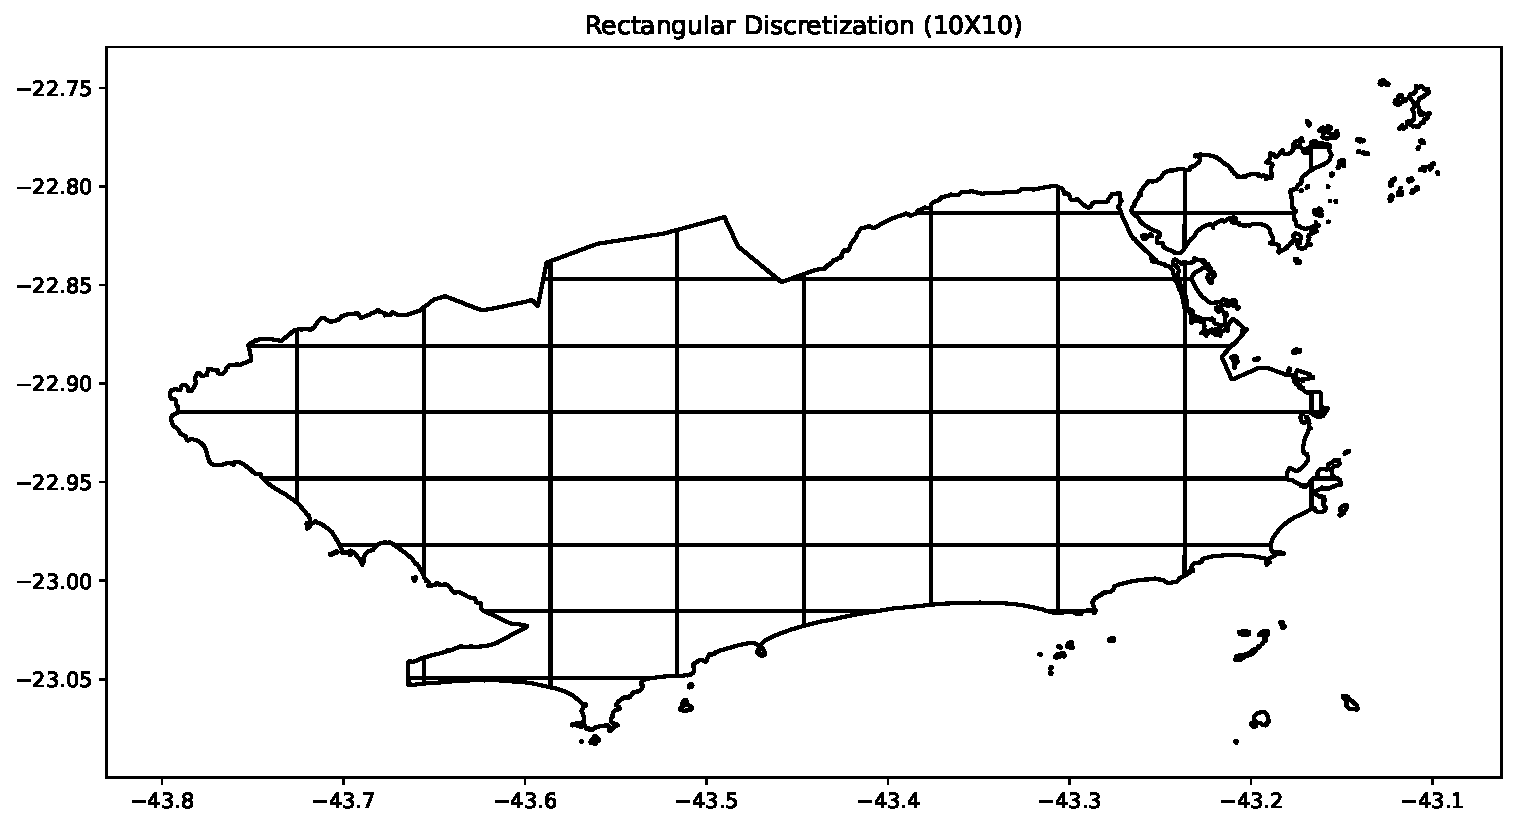
\includegraphics[scale=0.6]{disc_10x10.pdf}
\end{tabular}
\caption{\label{figurerect1010}
Space discretization of a region containing the city of Rio de Janeiro into $10 \times 10 = 100$ rectangles, 76 of which have nonempty intersection with the region and are shown in the figure.}
\end{figure}


\begin{figure}
\centering
\begin{tabular}{c}
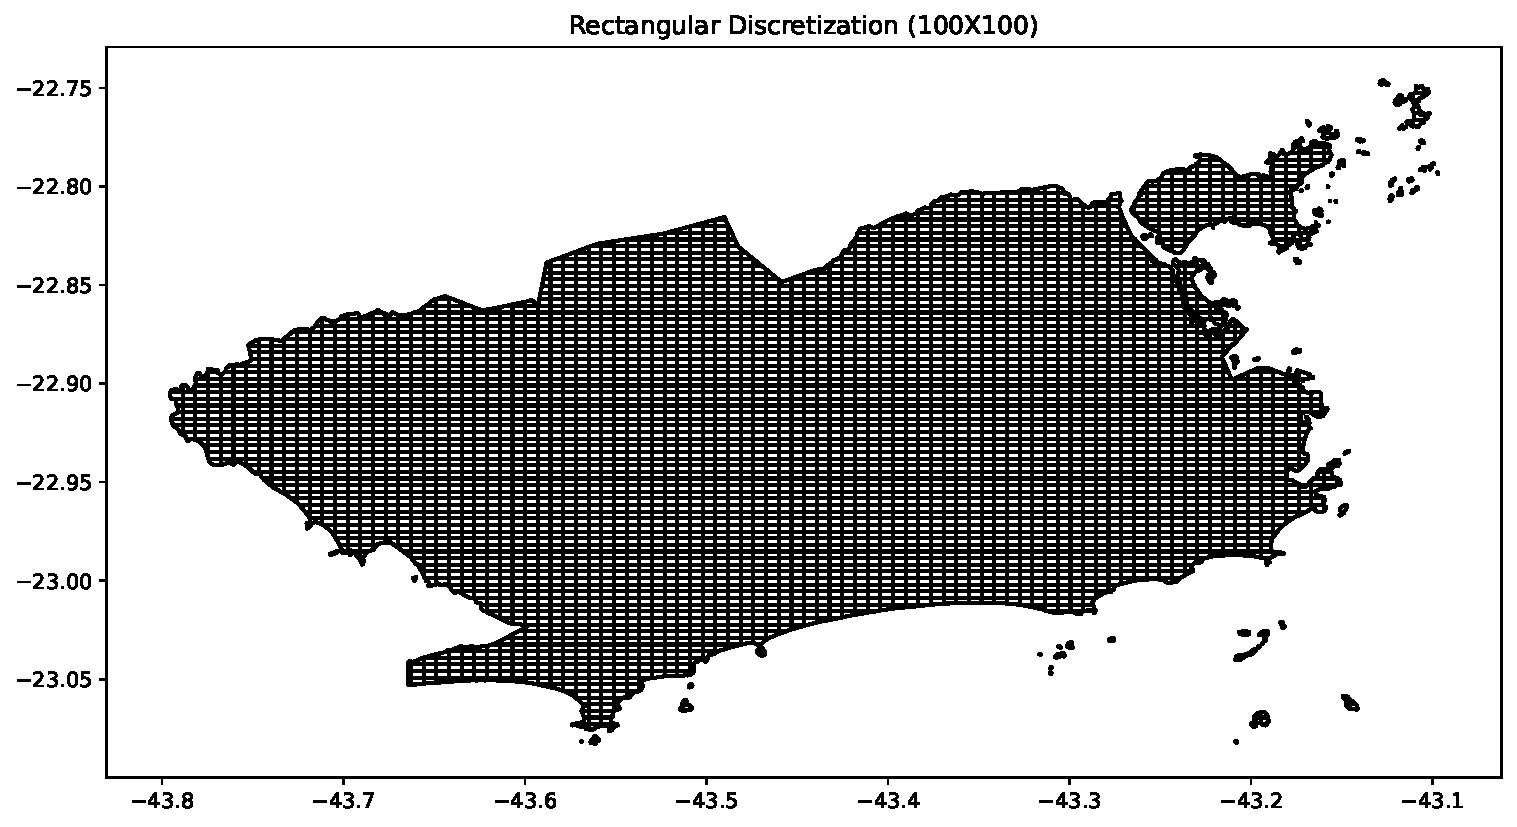
\includegraphics[scale=0.6]{disc_100x100.pdf}
\end{tabular}
\caption{\label{figurerect100100}
Space discretization of a region containing the city of Rio de Janeiro into $100 \times 100 = 10000$ rectangles, 4916 of which have nonempty intersection with the region and are shown in the figure.}
\end{figure}


\subsection{Equal Sized Hexagonal Space Discretization}

Another simple space discretization in LASPATED partitions the region into equal sized hexagons, in such a way that adjacent hexagons share a common edge.
(The Uber Python package \textit{H3} was used for the discretization.)
Figure~\ref{fig:uber7} shows a discretization of a region containing the city of Rio de Janeiro into hexagons using scale parameter equal to 7, and Figure~\ref{fig:uber8} shows a discretization of the same region into hexagons using scale parameter equal to 8.
Both discretizations were obtained with LASPATED.

\ignore{
LASPATED also provides an hexagonal discretization of the studied area.
This discretization is again obtained with LASPATED method {\textbf{add\_geo\_discretization}} now specifying 'H' for parameter \textbf{discr\_type} and an additional scale integer parameter \textbf{hex\_discr\_param} taking values between one and 16, where the smaller the integer the coarser the discretization.

\begin{lstlisting}[label={list:7},caption=Hexagonal discretization.]

# Hexagonal discretization with scale parameter 7
# The corresponding discretization for Rio de Janeiro city is given in  Figure 3
app.add_geo_discretization(
    discr_type='H',
    hex_discr_param=7
)

import matplotlib as plt
app.geo_discretization.boundary.plot()
plt.show()

# Hexagonal discretization with scale parameter 8
# The corresponding discretization for Rio de Janeiro city is given in  Figure 4
app.add_geo_discretization(
    discr_type='H',
    hex_discr_param=8
)

# Plotting the regions
app.geo_discretization.boundary.plot()
plt.show()
\end{lstlisting}
}

\begin{figure}
\centering
\begin{tabular}{c}
\includegraphics[scale=0.6]{disc_hex7.pdf}
\end{tabular}
\caption{\label{fig:uber7}
Space discretization of a region containing the city of Rio de Janeiro into hexagons using the Uber library H3 with scale parameter equal to $7$.}
\end{figure}


\begin{figure}
\centering
\begin{tabular}{c}
\includegraphics[scale=0.6]{disc_hex8.pdf}
\end{tabular}
\caption{\label{fig:uber8}
Space discretization of a region containing the city of Rio de Janeiro into hexagons using the Uber library H3 with scale parameter equal to $8$.}
\end{figure}


\subsection{Customized Space Discretization}

LASPATED also facilitates space discretization with customized subregions.
For example, Figure~\ref{fig:figuredistrict} obtained with LASPATED displays a customized discretization of the city of Rio de Janeiro into $160$~administrative districts.

\ignore{
First, a GeoDataFrame object containing the geometries of each subregion needs to be provided. 
Then the space discretization is obtained again with method {\textbf{add\_geo\_discretization}} specifying 'C' as \textbf{discr\_type} parameter and the GeoDataFrame object of the subregions as the additional parameter \textbf{custom\_data}. 
For instance, in Example \ref{list:8} where the studied area is the city of Rio de Janeiro, we take as subregions the administrative districts.
The corresponding GeoDataFrame object, denoted by custom\_map in the example, is obtained from the shapefile rio\_neighborhoods.shp of the districts of the city (this shape file can be found on the GitHub webpage of the project).

\begin{lstlisting}[label={list:8},caption=Custom discretization.]
import geopandas as gpd
custom_map = gpd.read_file(r'../Data/rio_de_janeiro_neighborhoods/rio_neighborhoods.shp')
app.add_geo_discretization('C', custom_data=custom_map)

# Plotting the regions
app.geo_discretization.boundary.plot()
plt.show()
\end{lstlisting}
}

\begin{figure}
\centering
\begin{tabular}{c}
\includegraphics[scale=0.6]{disc_custom.pdf}
\end{tabular}
\caption{\label{fig:figuredistrict}
Space discretization of a region containing the city of Rio de Janeiro into 160 administrative districts.\label{distfig}}
\end{figure}


\subsection{Discretization using Voronoi diagrams}

LASPATED also provides space discretization with Voronoi diagrams. Figure~\ref{figurevoronoi} obtained with LASPATED displays a discretization based on the Voronoi diagram given by the locations of ambulance stations in Rio de Janeiro.
Each zone includes the set of points that are closest to a specific station.

\begin{figure}
\centering
\begin{tabular}{c}
\includegraphics[scale=0.5]{voronoi_128_dots.pdf}
\end{tabular}
\caption{\label{figurevoronoi} Discretization of a region containing the city of Rio de Janeiro into 34 subregions given by the Voronoi diagram of ambulance stations in Rio de Janeiro.}
\end{figure}


\section{Additional Discretization Functionalities}
\label{sec:adddisc}

Often different discretizations are used for different purposes.
For example, different spatial attribute data such as population count and land use type may be provided using different space discretizations.
Consider two discretizations $D_{1}$ and $D_{2}$.
Let $\mathcal{I}_{1}$ be the index set of the subregions of discretization $D_{1}$, and let $\mathcal{I}_{2}$ be the index set of the subregions of discretization $D_{2}$.
In this context, LASPATED provides the following functionalities:
\begin{itemize}
\item
Given subregion indices $i_{1} \in \mathcal{I}_{1}$ and $i_{2} \in \mathcal{I}_{2}$, LASPATED computes the area $\mathcal{A}(i_{1},i_{2})$ of the intersection of subregions $i_{1}$ and $i_{2}$. Figure~\ref{fig:soil_use} displays a partition of Rio de Janeiro into 4 different types of soil use.
%Parameters gpd1 and gpd2 are the GeoDataFrames corresponding to discretizations \(D_{1}\) and \(D_{2}\). 
%The method returns the areas $\mathcal{A}(i,j)$ as a 2-D numpy array with the areas measured in square kilometers.
\item
Consider a given attribute, such as population count, and assume that the attribute value $P_{i_{1}}$ in each subregion $i_{1} \in \mathcal{I}_{1}$ of discretization $D_{1}$ is uniformly distributed with density $d_{i_{1}} = P_{i_{1}} / \mathcal{A}(i_{1})$, where $\mathcal{A}(i_{1})$ is the area of subregion~$i_{1}$.
We want to allocate this attribute value to the subregions of another discretization $D_{2}$.
LASPATED computes the value of the attribute allocated to subregion $i_{2} \in \mathcal{I}_{2}$ of discretization $D_{2}$ as $\displaystyle \sum_{i_{1} \in \mathcal{I}_{1}} d_{i_{1}} \mathcal{A}(i_{1},i_{2}) = \displaystyle \sum_{i_{1} \in \mathcal{I}_{1}} P_{i_{1}} \mathcal{A}(i_{1},i_{2}) / \mathcal{A}(i_{1})$. As an example, Figure~\ref{fig:soil_use} displays a partition of Rio de Janeiro into 4 different types of soil use and Laspated can be used to compute for every zone of a given discretization (for instance in rectangles or hexagones) the area of the different land types.
\ignore{
This calculation is simply obtained knowing attributes $P_{i_{1}}$ and areas $\mathcal{A}(i_{1})$ and $\mathcal{A}(i_{1},i_{2})$ (using get\_areas\_intersection).
The corresponding computation is done with LASPATED using method add\_geo\_variable.
In Example \ref{list:9}, we consider the attribute population.
We first read the corresponding shape file population.shp generating a GeoDataFrame object and filter only the columns "population" and "geometry".
This file can be found on the project GitHub page and gives the population in all the districts of the city of Rio de Janeiro.
Therefore, for this example Discretization $D_{1}$ is given by the districts of Rio de Janeiro (see Figure \ref{distfig}).
The GeoDataFrame object filtered as explained above is passed as an argument of method add\_geo\_variable.
The object app will contain information about the population of every elementary cell of discretization $D_{1}$ (see the next section).

If we assume the index set $\mathcal{I}_{1}$ for the discretization $D_{1}$ is partitioned into $k$ index sets $\mathcal{J}_{1}$, $\ldots$,$\mathcal{J}_{k}$: $\mathcal{J}=\sum_{i=1}^k \mathcal{J}_i$, then LASPATED method add\_geo\_variable can also be used to compute $\mathcal{A}_{i \ell} = \displaystyle \sum_{j \in \mathcal{J}_{\ell}} \mathcal{A}(i,j)$ for every $\ell=1,2,\ldots,k$, and $i \in \mathcal{I}$.
In Example \ref{list:9}, we read a shape file soil\_use.shp (available on the github page of the project) providing the different land types (we have 16 of them in this data) for the city of Rio de Janeiro.
Each elementary cell of this discretization contains one land type only.
We then filter the first two land types.
It then suffices to pass the corresponding GeoDataFrame object to method add\_geo\_variable.
The object app will contain information about the areas of land types 1 and 2 for every elementary
cell of discretization $D_{1}$ (see the next section).
}
\end{itemize}

\begin{figure}
    \centering
    \includegraphics[width=\textwidth]{soil_use.pdf}
    \caption{4 types of soil use in Rio de Janeiro.}
    \label{fig:soil_use}
\end{figure}

\ignore{
\begin{lstlisting}[label={list:9},caption=Additional discretization features.]
import geopandas as gpd
population = gpd.read_file(r'../Data/regressors/population/population.shp')
population = population[["population", "geometry"]].copy()
app.add_geo_variable(population)

land_use = gpd.read_file(r'../Data/regressors/soil_use/soil_use.shp')
land_use = land_use[["type_{1}", "type_{2}", "geometry"]].copy()
app.add_geo_variable(land_use)
\end{lstlisting}
}


\ignore{
\section{Retrieving discretization data from the aggregator and writing discretized data in files}
\label{sec:retriev}

LASPATED spatio-temporal discretizations are stored in \textbf{app.events\_data} and \textbf{app.geo\_discretization} which are two dataframes.
Dataframe \textbf{app.events\_data} has the same columns as the events dataframe loaded in Section 2, plus time and spatial discretization columns.
For each event, the time index discretizations are added with the columns named \textbf{tdiscr\_i}, $i = 0,\ldots,T-1$, with $T$ being the number of time index  discretizations defined. Custom column names may be provided in the \textbf{app.add\_time\_discretization} method, with the default \textbf{column\_name} parameter.
Similarly, the spatial discretization is added with the default name \textbf{gdiscr}.
For each event, \textbf{gdiscr} is the index of the region where the event took place.
The regions defined in the spatial discretization are fully detailed in the \textbf{app.geo\_discretization} dataframe. For each region, the dataframe stores its index, the list of indexes of neighboring regions, the latitude and longitude of the centroid of the region, and columns with its additional discretization features (for instance population, areas of different land types, see Section
\ref{sec:adddisc} and Example \ref{list:9} for these features). 

LASPATED  method \textbf{get\_events\_aggregated()} returns a numpy multidimensional array of lists $A$, where $A[t_{0},t_{1},\ldots,t_{T-1},g,f_{0},f_{1},\ldots,f_{F-1}]$ is a list containing the number of events observed in app.events\_data for time discretizations $t_{0},\ldots,t_{T-1}$, spatial discretization $g$ and features $f_{0},\ldots,f_{F-1}$ with $T$ being the number of time discretizations and $F$ the number of features.
Example \ref{list:10} shows how to call the method.

\begin{lstlisting}[label={list:10},caption=Aggregating events by discretization.]
app.add_events_data(events, datetime_col='date_time', lat_col='lat', lon_col="long", feature_cols=['priority'])

app.add_time_discretization('m', 30, 30*48) # tdiscr_0
app.add_time_discretization('D', 1, 7) tdiscr_{1}

app.add_geo_discretization(
    discr_type='R',
    rect_discr_param_x=10,
    rect_discr_param_y=10
)

events_agg = app.get_events_aggregated()

# Axis are respectively: tdiscr_0, tdiscr_{1}, gdiscr, priority
print(events_agg.shape)
\end{lstlisting}

The method \textbf{write\_files} saves both dataframes as csv files. The first parameter of this method is the path of the file storing the information in \textbf{app.geo\_discretization} while the second parameter is the path of the file storing the information in \textbf{app.events\_data}.

\begin{lstlisting}[label={list:10},caption=Writing the discretized data to a file.]
app.write_files("geo_discretization.csv", "events.csv")
\end{lstlisting}
}


\ignore{
\section{Model calibration} \label{sec:modelcalibration}

\subsection{Matlab LASPATED calibration functions}

\subsubsection{Calibration of the models for fixed penalties}

LASPATED function laspated calibrates the models
from Sections \ref{sec:model1} and \ref{sec:modelcov}
for fixed penalties $w_{i,j}$ and $W_G$ using
the projected gradient method with 
Armijo line search along the feasible
direction (see the pseudo code of this variant
of projected gradient in the appendix).
The user can also find on the GitHub repository of the
library, function {\tt{projectedGradientArmijoBoundary}} which calibrates 
the models using
projected gradient with Armijo line search along
the boundary (given in the Appendix) but this variant of projected gradient 
is usually slower than projected gradient with Armijo search along
the feasible direction
and is therefore not used by laspated function.
The documentation of function {\tt{projectedGradientArmijoBoundary}} is given in the header of file
projectedGradientArmijoBoundary.
In this section, we focus on laspated function.

A typical call to laspated is
\begin{center}
\begin{tabular}{l}
[lambda,obj]=laspated(model, nbObservations, nbArrivals, T, R, C, durations, Groups,\\
\hspace*{3.6cm}whichgroup, weight, sigma, iterMax, epsilon, lambda0, params).
\end{tabular}
\end{center}

This function has a variable {\tt{model}}
which is a string 
which is {\tt{noreg}} to calibrate the model (without regression)
of Section \ref{sec:model1} and 
{\tt{reg}} to calibrate the model (with regression)
of Section \ref{sec:modelcov} (other values of this string
will generate the message {\tt{Invalid model name}}).

Function laspated has also the following input variables:
\begin{itemize}
\item nbObservations, which gives the number of observations
for every possible combinations of arrival types, time steps,
and regions. More precisely, if {\tt{model}}={\tt{noreg}} then
nbObservations is a 3 dimensional array with nbObservations(c,i,t) the number
of observations for 
arrival type with index c, region with index i, and
time window with index t
(this is parameter $N_{c,i,t}$ of the model)
and if {\tt{model}}={\tt{reg}} then nbObservations(c,d,t,i) is the number
of observations for arrival type $c$, day or holiday $d$,
time window with index t, and region with index i (this is parameter
$N_{c,d,t,i}$ of Example \ref{excov}).
\item nbArrivals: array providing the number of arrivals.
More precisely,  if {\tt{model}}={\tt{noreg}} then
this is a 3 dimensional array with nbArrivals(c,i,t)
the total number of arrivals observed for time window t,
region i, arrival type c (this is parameter $M_{c,i,t}$ of the model)
and if {\tt{model}}={\tt{reg}} then 
nbArrivals(c,d,t,i) is the number
of arrivals for arrival type $c$, day or holiday $d$,
time window with index t, and region with index i
(this is parameter $M_{c,d,t,i}$ of the model);
\item T: number of discretized time intervals (this is $|\mathcal{T}|$);
\item R: number of regions (this is $|\mathcal{I}|$);
\item C: number of arrival types (this is $|\mathcal{C}|$)
\item durations: 1-dimensional array with durations(t) the duration
of time interval with index t;
\item sigma: this is the value of parameter $\sigma$
in the pseudo-code of the Appendix for projected gradient with Armijo line search along the feasible
direction ($\sigma=0.5$ in the experiments reported in this section);
\item iterMax: maximal number of iterations for projected gradient; this is parameter MaxNumberIteration for the pseudo-code in the Appendix;
\item epsilon: if {\tt{model}}={\tt{noreg}} this is parameter $\varepsilon$ in \eqref{eqn:Ceps}
and if {\tt{model}}={\tt{reg}}
this is parameter 
$\varepsilon$ in
\eqref{eqn:feassetref1};
\item lambda0: initial value $\lambda_{0}$ of $\lambda$ (see the pseudo-code in the Appendix); when
 model=noreg, this is a 3 dimensional array with lambda0(c,i,t) an
initial guess for the vector of intensities 
$\lambda_{c,i,t}$ for 
 time window with index t, region with index i, arrival type $c$ with lambda0 satisfying the constraints in \eqref{eqn:Ceps}  and
 when model=reg
 this is an initial value for $\beta=(\beta_{c,d,t})_{c,d,t}$
which needs to satisfy \eqref{eqn:feassetref1}.
\end{itemize}
Function laspated has also a structure params with parameters
that depend on the model. 

When {\tt{model}}={\tt{noreg}}, then params
has the following fields:
\begin{itemize}
\item params.Groups: cell array with params.Groups\{1,i\} an array
where params.Groups\{1,i\}(j) is the index of $j$th time interval which is
in time group with index i (recall the time groups are $G \in \mathcal{G}$ for loss function \eqref{eqn:regularization1}). 
\item params.whichgroup: 1-dimensional array of size $T$ where params.whichgroup(t) is the index
of the time group which contains time interval with index t.
\item params.weight: 1-dimensional array with 
params.weight(i) the weight $W_G$ in loss function \eqref{eqn:regularization1} corresponding to time group $G$ with index i.
\item params.type(i) is the type of region (with index)
i (the type of a region is a positive integer
coding the type of the region, for instance
we could consider regressors
as in the model with covariates
from Section \ref{sec:model1}
and consider the most important
regressor in the
region, say the land type with largest
area); it is possible not to use
this type information defining all types
equal (say to 1);
\item params.distance: 2-dimensional array with 
params.distance(i,j) the distance between the centroids
of regions with indexes i and j;
\item params.alpha: this is the common value of
weights $w_{i j}$ in loss function
\eqref{eqn:regularization1} which are equal to params.alpha only
when regions with indexes $i$ and $j$ are 
neighbors and are
of the same type, i.e., when
type(i)=type(j).
\end{itemize}
When {\tt{model}}={\tt{reg}}, then params
has the following fields:
\begin{itemize}
\item params.D: number of days plus holidays;
\item params.indexBeta: 
a vector of indexes for $\beta$ such that
$\beta_{c,d,t}(j)$ is 
lambda(params.indexBeta(c,d,t,j)) (lambda being the optimization variable);
\item params.regressor: params.regressor(j,i) is the value of  regressor
j for region with index i;
\item params.nbRegressors: number of regressors;
\item params.sizex: number of entries in vector $\beta=(\beta_{c,d,t})_{c,d,t}$.
\end{itemize}

The outputs are
\begin{itemize}
\item lambda: when variable {\tt{model}}
is {\tt{noreg}} lambda is an estimated optimal solution of
problem \eqref{eqn:model0}. More precisely, this is
a 3 dimensional array with lambda(c,i,t) the optimal  intensity 
$\lambda_{c,i,t}$ for 
 time window t, region i, arrival type $c$. When variable 
 {\tt{model}}
is {\tt{reg}} lambda is an estimated optimal value
for the problem of minimizing loss function 
\eqref{eqn:lossf} under the constraints
\eqref{eqn:feassetref1}. This variable lambda
is a 1 dimensional vector with lambda(params.indexBeta(c,d,t,j))
an optimal value for $\beta_{c,d,t}(j)$. 
\item obj: when variable {\tt{model}}
is {\tt{noreg}} this is the estimated optimal value
of problem \eqref{eqn:model0} along iterations of the method and when {\tt{model}}
is {\tt{reg}} this is the estimated optimal value
along iterations of the method applied to
the problem of minimizing loss function 
\eqref{eqn:lossf} under the constraints
\eqref{eqn:feassetref1}.
\end{itemize}

\subsubsection{Calibration of penalties}

The calibration of parameters $w_{i,j}$ 
and $W_G$ in loss function 
\eqref{eqn:regularization1}
can be done calling function
crossValidation
of LASPATED library. This function uses cross validation
to estimate a value $\alpha=w_{i,j}=W_G$
common to all pairs of neighboring regions $i,j$
and  all groups $G$.
A call to this function is
\begin{center}
\begin{tabular}{l}
[cputime,weight,lambda]=crossValidation(model, sample, T, R, C, sigma, lambda0, iterMax, proportion,\\
\hspace{6.5cm}epsilon, durations, Groups, whichgroup, weights, params).
\end{tabular}
\end{center}
The input variables which have the names of the input variables
of laspated function have the same meaning as before.
Additionally we have the following input variables:
\begin{itemize}
\item sample which is the sample of arrivals.
More precisely, sample is a 
4-dimensional array with 
sample(t,i,c,j) the $j$th observation
for time window $t$, region $i$, and arrival type
$c$;
\item proportion is a real in the interval $(0,1)$
(typically 0.2) which is the proportion of data
used in every estimation block of cross validation
while the proportion (1-proportion) is the proportion of
data used for validation (in cross validation).
\item weights is an array of candidate weights
for $w_{i,j}$ and $W_G$.
\end{itemize}

params is a structure
with the fields
params.neighbors=neighbors, params.type=type; params.distance=distance,
params.alpha=1, which have the same meaning as before.


\subsubsection{Matlab examples}

\par {\textbf{Simulated data, model without regressors.}} The implementation corresponding to the example 
described in this section is  given in file laspatedex1noreg.
Running the corresponding function
$$
{\tt{[weight,lambda,obj]=laspatedex1noreg()}}
$$
builds the data corresponding to this example and runs laspated calibration function for the model without regressors of Section~\ref{sec:model1} for a set of penalizations.
It also runs cross validation.
The output weight is the best penalization found by cross validation and lambda is the vector of intensities.
}

\section{LASPATED Calibration Functions}
\label{sec:calib}

LASPATED provides Matlab and C++ functions for the calibration of models as in Section~\ref{sec:model1} for given values of weights $W_{G}$ and $w_{i,j}$, by solving
problem~\eqref{eqn:reformmodel1} using the projected gradient method with Armijo line search along a feasible direction or along the boundary.

LASPATED also provides Matlab and C++ cross validation functions for the selection of weights $W_{G}$ and $w_{i,j}$ and the computation of the corresponding optimal intensities
$\lambda_{c.i.t}$ that solve problem~\eqref{eqn:reformmodel1}
for the selected weights.

LASPATED also provides Matlab and C++ functions for the
calibration of models with covariates, as in  Section~\ref{sec:modelcov}.
More precisely, it solves optimization problem~\eqref{optlikelihbeta} using projected gradient with Armijo line search along a feasible direction or along the boundary.

LASPATED includes the test examples for the calibration functions described in the next section.


\section{Numerical Examples}
\label{sec:examples}

In this section we demonstrate the LASPATED calibration functions using examples with simulated and real data.
In all examples, the models were calibrated using the projected gradient method with Armijo search along a feasible direction, as described in section~\ref{sec:opt_sol}, using $\overline{\Delta} = 2$ and $\sigma = 0.5$.


\subsection{Numerical Examples with Artificial Data without Covariates}
\label{sec:simulated example}

In these examples, points arrive in $2$-dimensional space and over time according to a periodic non-homogeneous Poisson process.
There is only one type of point, thus $|\mathcal{C}| = 1$, and hence the type notation~$c$ is omitted.
The region under consideration is $\mathcal{S} = [0,10]^2$, as shown in Figure~\ref{figureserr}. 

\begin{figure}
\centering
\begin{tabular}{c}
\includegraphics[scale=0.65]{Sites.pdf}
\end{tabular}
\caption{\label{figureserr}
Example region $\mathcal{S} = [0,10]^2$.
The intensity function $\lambda$ is different in the blue and red subregions, but the user does not know about these subregions.
For estimation purposes, the user discretizes $\mathcal{S}$ into $10 \times 10 = 100$ square zones.
%The red (respectively blue) zones have red squares (respectively blue circles) in their centers.
%The red zones are in the bottom left and upper right of the region while the blue zones are in the bottom right and upper left of the region.
}
\end{figure}

The region $\mathcal{S}$ is partitioned into two subsets $\mathcal{S} = \mathcal{B} \cup \mathcal{R}$, with $\mathcal{B} = [0,5] \times (5,10] \cup (5,10] \times [0,5]$ and $\mathcal{R} = [0,5] \times [0,5] \cup (5,10] \times (5,10]$.





\subsubsection{Example~1}
\label{sec:example 1}

In this example, the rate function $\lambda : \mathcal{S} \times [0,T] \mapsto \RR_{+}$ is different on $\mathcal{B}$ and on $\mathcal{R}$, and is periodic with period~$2$, as follows:
\[
\lambda(s,t) \ \ = \ \ \left\{\begin{array}{lcl}
0.1 & \mbox{if} & s \in \mathcal{B} \mbox{ and } t \in (2k,2k+1] \mbox{ for some } k \in \NN, \\
0.5 & \mbox{if} & s \in \mathcal{B} \mbox{ and } t \in (2k-1,2k] \mbox{ for some } k \in \NN, \\
0.5 & \mbox{if} & s \in \mathcal{R} \mbox{ and } t \in (2k,2k+1] \mbox{ for some } k \in \NN, \\
0.1 & \mbox{if} & s \in \mathcal{R} \mbox{ and } t \in (2k-1,2k] \mbox{ for some } k \in \NN.
\end{array}\right.
\]
This rate function is represented in Figure~\ref{figuresex1}(a) (for time intervals that start at odd times) and Figure~\ref{figuresex1}(b) (for time intervals that start at even times). 

\begin{figure}
\centering
\resizebox{\textwidth}{!}{
%\scalebox{0.75}{
\begin{tabular}{cc}
\includegraphics[scale=0.5]{lambdaconstanteven.pdf} &
\includegraphics[scale=0.5]{lambdaconstantodd.pdf} \\
$\hspace*{0.6cm}$(a) Time intervals that start at odd times & $\hspace*{0.6cm}$(b) Time intervals that start at even times
\end{tabular}}
\caption{\label{figuresex1}
Intensities as a function of location, for time intervals that start at odd times and even times.}
\end{figure}

The user knows the region $\mathcal{S}$ and that $|\mathcal{C}| = 1$, but does not know about the subregions $\mathcal{B}$ and $\mathcal{R}$ that affect the intensity function $\lambda$, and does not know that $\lambda$ is periodic with period~$2$.
For estimation purposes, the user discretizes $\mathcal{S}$ into $100$~square zones of unit area each, as shown in Figure~\ref{figureserr}.
%These squares of unit area correspond to the zones of the discrete model components.
Thus $\mathcal{I} = \mathcal{I}_{\mathcal{B}} \cup \mathcal{I}_{\mathcal{R}}$ indexes two types of zones, but this is not known by the user:
\begin{itemize}
\item
$\mathcal{I}_{\mathcal{B}}$ indexes $50$~blue zones (with blue circles in their centers in Figure~\ref{figureserr}); there are $25$~blue zones in the bottom right and $25$~blue zones in the upper left of the region;
\item
$\mathcal{I}_{\mathcal{R}}$ indexes $50$ red zones (with red squares in their centers in Figure~\ref{figureserr}); there are $25$~red zones on the bottom left and $25$~red zones in the upper right of the region.
\end{itemize}
Also, for estimation purposes, the user discretizes time into $28$~time intervals of length~$1$ each.
Thus, the estimates are denoted with $\lambda_{i,t}$ for $i \in \mathcal{I}$ and $t \in \mathcal{T} \defi \{1,\ldots,28\}$.
Given arrival data $M_{i,t,n}$ for $i \in \mathcal{I}$, $t \in \mathcal{T}$, and $n = 1,\ldots,N_{i,t}$, the regularized loss function in~\eqref{eqn:regularization1} is used to estimate $\lambda_{i,t}$.
The penalty coefficients are $w_{i,j} = w > 0$ when $i,j$ are neighboring zones, and $w_{i,j} = 0$ otherwise, where $w$ will be varied as described later. Two zones are neighbors if their borders share an edge.

We consider two partitions $\mathcal{G}_{2}$ and $\mathcal{G}_{4}$ of time intervals $\mathcal{T}$ in~\eqref{eqn:regularization1}.
For partition $\mathcal{G}_{2}$, the time groups are $G_{0} = \{2k \, : \, k=1,\ldots,14\}$ and $G_{1} = \{2k+1 \, : \, k=0,1,\ldots,13\}$.
For partition $\mathcal{G}_{4}$, the time groups are $G_{0} = \{4k \, : \, k=1,\ldots,7\}$, $G_{1} = \{4k+1 \, : \, k=0,1,\ldots,6\}$, $G_{2} = \{4k+2 \, : \, k=0,1,\ldots,6\}$, and $G_{3} = \{4k+3 \, : \, k=0,1,\ldots,6\}$.
For both partitions, penalty coefficients $W_{G} = w$ for all groups~$G$ (note that all groups have the same cardinality so that it seems reasonable to choose the same weights for different groups).
Also, $\varepsilon = 0.001$ in~\eqref{eqn:Ceps}.

\ignore{
In the red (respectively blue) zones the arrival process is Poisson with intensity $\lambda_{r}(\cdot)$ (respectively $\lambda_{b}(\cdot)$) over time windows of the same duration $\mathcal{D}_{t}=1$ time unit, a time unit being of 6 hours.
Also $\lambda_{r}(\cdot)$ and $\lambda_{b}(\cdot)$ are periodic with period 28; say a period is of 7 days with each day divided into 4 time windows of the same duration 6 hours, so that we have $T=28$ time windows of 6 hours in  a period.
For convenience, zones are numbered from left to right and from bottom to top.
For instance, the 5 red bottom zones are, from left to right, zones 1, 2, 3, 4, and 5; the 5 blue bottom zones are, from left to right, zones 6, 7, 8, 9, and 10.
For the zones immediately above, the red zones are, from left to right, zones 11, 12, 13, 14, and 15, while the blue zones are, from left to right, zones 16, 17, 18, 19, and 20, and so on...
Given a set of arrivals $M_{1,i,t,n}$ for zone $i$, time $t=1,\ldots,T$, $n=1,\ldots,N_{1,i,t}$ (we used the notation of Section~\ref{sec:modelcalib} to index the observations, knowing that we have only one arrival type $c=1$ observed for time windows $t=1,\ldots,T$), our goal is to estimate intensities $\lambda_{r,i,t}$ in red zones $i$ and $\lambda_{b,i,t}$ in blue zones $i$ for every time window $t=1$,$\ldots$, $T=28$ within a period.
The true intensities in red zones $i$ are given by
$$
\begin{array}{l}
\lambda_{r,i,2k+1}=0.5,\;k=0,1,\ldots,13,\\
\lambda_{r,i,2k}=0.1,\;k=1,\ldots,14,
\end{array}
$$
and in blue zones $i$ by
$$
\begin{array}{l}
\lambda_{b,i,2k+1}=0.1,\;k=0,1,\ldots,13,\\
\lambda_{b,i,2k}=0.5,\;k=1,\ldots,14.
\end{array}
$$
It can be seen that the sequence of intensities is actually periodic with period 2 but we do not assume we know the period is 2: we only assume for estimation of the intensities that these intensities are periodic with period 28 (one week).
We also do not assume that we know that intensities are all equal in red zones and are all equal in blue
zones.
However, to show the importance of regularization used in loss function~\eqref{eqn:regularization1} of the model of Section~\ref{sec:model1}, we use penalizing coefficients $w_{i,j} = w > 0$ when $i,j$ are neighboring blue zones and when $i,j$ are neighboring red zones (two zones are neighbors if they
share a border, i.e., they have a nonempty intersection).
For this loss function~\eqref{eqn:regularization1}, we also create four time groups forming a partition of $\{1,2,\ldots,28\}$, more specifically time groups $\{4k+1,k=0,1,\ldots,6\}$, $\{4k+2,k=0,1,\ldots,6\}$, $\{4k+3,k=0,1,\ldots,6\}$, and $\{4k,k=1,\ldots,7\}$.
We also take $W_{G} = w$ for all groups $G$ (note that all groups have the same cardinality otherwise different weights may be chosen for different groups).
Finally we take $\varepsilon = 0.001$ in~\eqref{eqn:Ceps}.

We estimate the intensities of the Poisson process using the regularized estimator proposed in Section~\ref{sec:model1} selecting equal penalties $p = w_{ij} = W_{G}$ for all time groups~$G$ and for neighboring blue zones and neighboring red zones varying in the set
$$
\begin{array}{l}
\left\{0,0.01,0.05,0.1,1,5,10,20,30,40,50,60,70,80,90,100,110,120,\right.\\
\left. 130,140,150,160,170, 180,190,200,210,220,230,240,250,260,270,280,\right.\\
\left. 290,300,310,320,330,340,350,360,370,380,390,400\right\}.
\end{array}
$$
}

For any value of the penalty parameter $w$, let $\hat{\lambda}^{w}_{i,t}$ denote the estimator of $\lambda_{i,t}$ produced by~\eqref{eqn:model0}.
Note that when the penalty parameter $w = 0$, then $\hat{\lambda}^{0}_{i,t}$ reduces to the empirical estimator of the intensities, which is the mean rate of arrivals in zone~$i$ and time interval~$t$.
For a range of values of the penalty parameter~$w$, we computed the estimates $\hat{\lambda}^{w}_{i,t}$, and Figure~\ref{figureserr1} shows the mean (over all zones~$i$ and time intervals~$t$) relative error given by
\if{
$$\frac{100}{T|\mathcal{I}|}\sum_{t=1}^{T} \sum_{i \in \mathcal{I}} 
\left|\frac{ \lambda_{c,i,t} - {\hat{\lambda}}_{c,i,t}^{p}}{\lambda_{c,i,t}}\right|
$$
}\fi
\[
\frac{1}{|\mathcal{I}||\mathcal{T}|} \sum_{i \in \mathcal{I}} \sum_{t \in \mathcal{T}}
\left|\frac{\lambda_{i,t} - \hat{\lambda}^{w}_{i,t}}{\lambda_{i,t}}\right|
\]
as a function of penalty parameter~$w$, for different values of $N_{i,t}$.
Figure~\ref{figureserr1} shows the mean relative errors for the following four estimators: estimator with partition $\mathcal{G}_{4}$ of time intervals and with neighbor-based spatial regularization (legend ``4 groups, neighbors'' in the figure), estimator with partition $\mathcal{G}_{4}$ of time intervals and without spatial regularization (legend ``4 groups, no neighbors'' in the figure), estimator with partition $\mathcal{G}_{2}$ of time intervals and with neighbor-based spatial regularization (legend ``2 groups, neighbors'' in the figure), and estimator with partition $\mathcal{G}_{2}$ of time intervals and without spatial regularization (legend ``2 groups, no neighbors'' in the figure).
Figure~\ref{figureserr1} presents results for four values of the sample size: $N_{i,t} = 14$ periods observed, $N_{i,t} = 140$ periods observed, $N_{i,t} = 700$ periods observed, and $N_{i,t} = 7000$ periods observed.
Figure~\ref{figureserr1} also shows, for the three larger sample sizes, the mean relative error obtained by choosing the penalty parameter~$w$ by cross validation as follows:
The data are partitioned into $5$ subsets.
Then, for each of $5$~replications we used one of the data subsets (a different subset for each replication, with 20\% of data used for training) to compute $\hat{\lambda}^{w}_{i,t}$ with partition $\mathcal{G}_{2}$ of time intervals and with neighbor-based spatial regularization for a range of values of~$w$, and we used the remaining data to compute the out-of-sample likelihood value for each value of~$w$.
Then we determined the penalty parameter~$w^*$ that maximizes the average out-of-sample likelihood value over the $5$~replications.
Figure~\ref{figureserr1} shows the mean relative error for the resulting cross validation estimator with partition $\mathcal{G}_{2}$ of time intervals and with neighbor-based spatial regularization using the penalty parameter~$w^*$.
Note that the empirical estimator, with $w = 0$, does not depend on the partition of time intervals and the neighbor structure, and therefore is given by all four estimators described above at $w = 0$.
Table~\ref{tabnoreg} shows the minimum mean relative errors over different values of penalty parameter~$w$, as well as the values of~$w$ that attain the minimum, for each of the four estimators, plus the mean relative errors of the cross validation estimator (using the penalty parameter~$w^*$) and the empirical estimator ($w = 0$), for each of the four sample sizes considered in Figure~\ref{figureserr1}.


\begin{table}
\centering
\begin{tabular}{|c|c|c|c|c|c|c|}
\hline
Sample size $N_{i,t}$ & Reg 1 & Reg 2 & Reg 3 & Reg 4 & CV & Emp \\
\hline
14 & 0.47/2 & 0.61/2  & 0.44/2  & 0.47/1.6  &  -  & 1.22/0  \\  
\hline
140  & 0.14/0.08  &  0.21/1.2  &  0.12/0.06 &  0.16/0.06  &  0.17/0.2  & 0.40/0\\
\hline
700 &  0.06/0.012 & 0.09/0.032  & 0.05/0.008  & 0.06/0.012  &  0.13/0.04  & 0.17/0 \\
\hline
7000 & 0.02/0.001 & 0.03/0.002 & 0.02/0.001 & 0.02/0.001 & 0.10/0.003 & 0.06/0 \\
\hline
\end{tabular}
% \begin{table}
% \centering
% \begin{tabular}{|c|c|c|c|c|c|c|}
% \hline
% Sample size $N_{i,t}$ & Reg 1 & Reg 2 & Reg 3 & Reg 4 & CV & Emp \\
% \hline
% 28 & 0.28/40  & 0.46/39  & 0.29/29  & 0.37/69  & 0.45/10   &1.2/0  \\  
% \hline
% 280  & 0.1/80  & 0.16/270  & 0.07/60  & 0.11/150  & 0.10/20   & 0.4/0\\
% \hline
% 1400 &  0.038/320 & 0.07/360  & 0.034/220  & 0.051/300  &  0.045/60  & 0.18/0 \\
% \hline
% 14000 &  0.028/400 & 0.036/400  & 0.022/400  & 0.026/400  &  0.025/220  &  0.058/0\\
% \hline
% \end{tabular}
\caption{\label{tabnoreg}
The column headings denote the estimators as follows: Reg 1: estimator with partition $\mathcal{G}_{4}$ of time intervals and with neighbor-based spatial regularization; Reg 2: estimator with partition $\mathcal{G}_{4}$ of time intervals and without spatial regularization; Reg 3: estimator with partition $\mathcal{G}_{2}$ of time intervals and with neighbor-based spatial regularization; Reg 4: estimator with partition $\mathcal{G}_{2}$ of time intervals and without spatial regularization; CV: cross validation; Emp: empirical estimator.
For each sample size and for each estimator Reg 1, Reg 2, Reg 3, Reg 4, each cell of the table gives two numbers separated by a slash (/): the first number is the minimum mean relative error over different values of penalty parameter~$w$, and the second number is the value of~$w$ that attain the minimum.
For the cross validation estimator, the first number is the mean relative error using penalty parameter~$w^*$, and the second number is the value of~$w^*$.
For the empirical estimator, the first number is the mean relative error using penalty parameter~$w = 0$.
}
\end{table}

\if{

\begin{table}
\centering
\begin{tabular}{|c|c|c|c|c|c|c|}
\hline
Sample size $N_{i,t}$ & Reg 1 & Reg 2 & Reg 3 & Reg 4 & CV & Emp \\
\hline
14 & 0.30/10 & 0.46/10 & 0.35/5 & 0.26/0.01 & - & 1.19/0  \\  
\hline
140  & 0.21/1  & 0.22/3   &  0.22/1 &  0.26/1  &  0.21/1  & 0.39/0 \\
\hline
700 &  0.05/0.02  & 0.07/0.03  & 0.04/0.02 & 0.05/0.03  &  0.12/0.1  & 0.08/0.01 \\
\hline
7000 &  0.05/0 & 0.04/0.01 & 0.05/0 & 0.05/0.01 & 0.15/0.01 & 0.05/0 \\ 
\hline
\end{tabular}



\caption{\label{tabnoreg2} For each sample size and for each estimator, each cell of the table gives two numbers separated by a slash (/): the first number is the minimum mean relative error over different values of penalty parameter~$w$, and the second number is the value of~$w$ that attain the minimum.
The column headings denote the estimators as follows: Reg 1: estimator with partition $\mathcal{G}_{4}$ of time intervals and with neighbor-based spatial regularization; Reg 2: estimator with partition $\mathcal{G}_{4}$ of time intervals and without spatial regularization; Reg 3: estimator with partition $\mathcal{G}_{2}$ of time intervals and with neighbor-based spatial regularization; Reg 4: estimator with partition $\mathcal{G}_{2}$ of time intervals and without spatial regularization; CV: cross validation; Emp: empirical estimator.}
\end{table}

}\fi

% 140   => 0.214/1, 
% 700   => 0.072/0.04, 
% 7000  => 0.091/0.01

\begin{figure}
\centering
\resizebox{\textwidth}{!}{
%\scalebox{0.75}{
\begin{tabular}{cc}
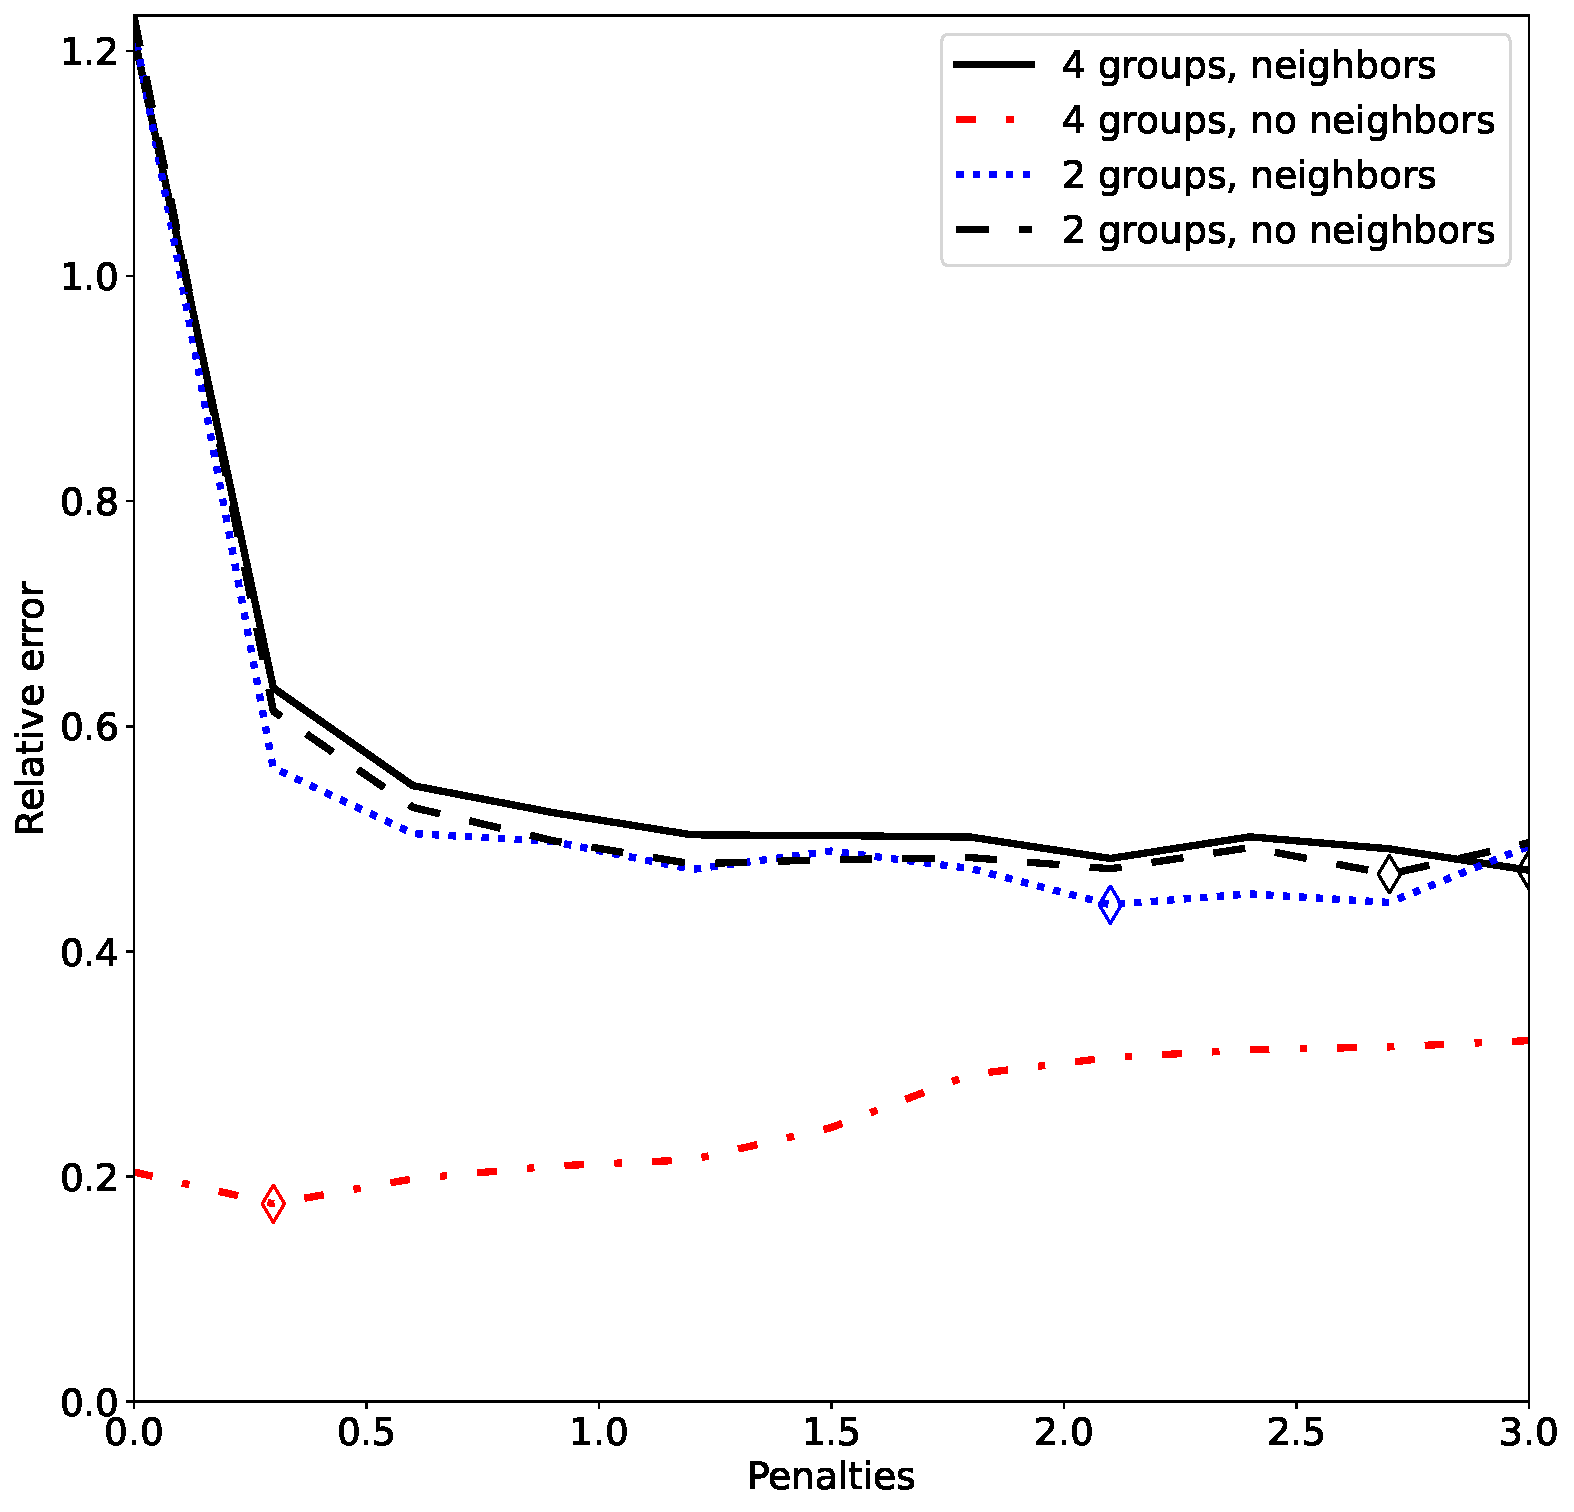
\includegraphics[scale=0.3]{2weeks_Color_Unknown_v3.pdf} &
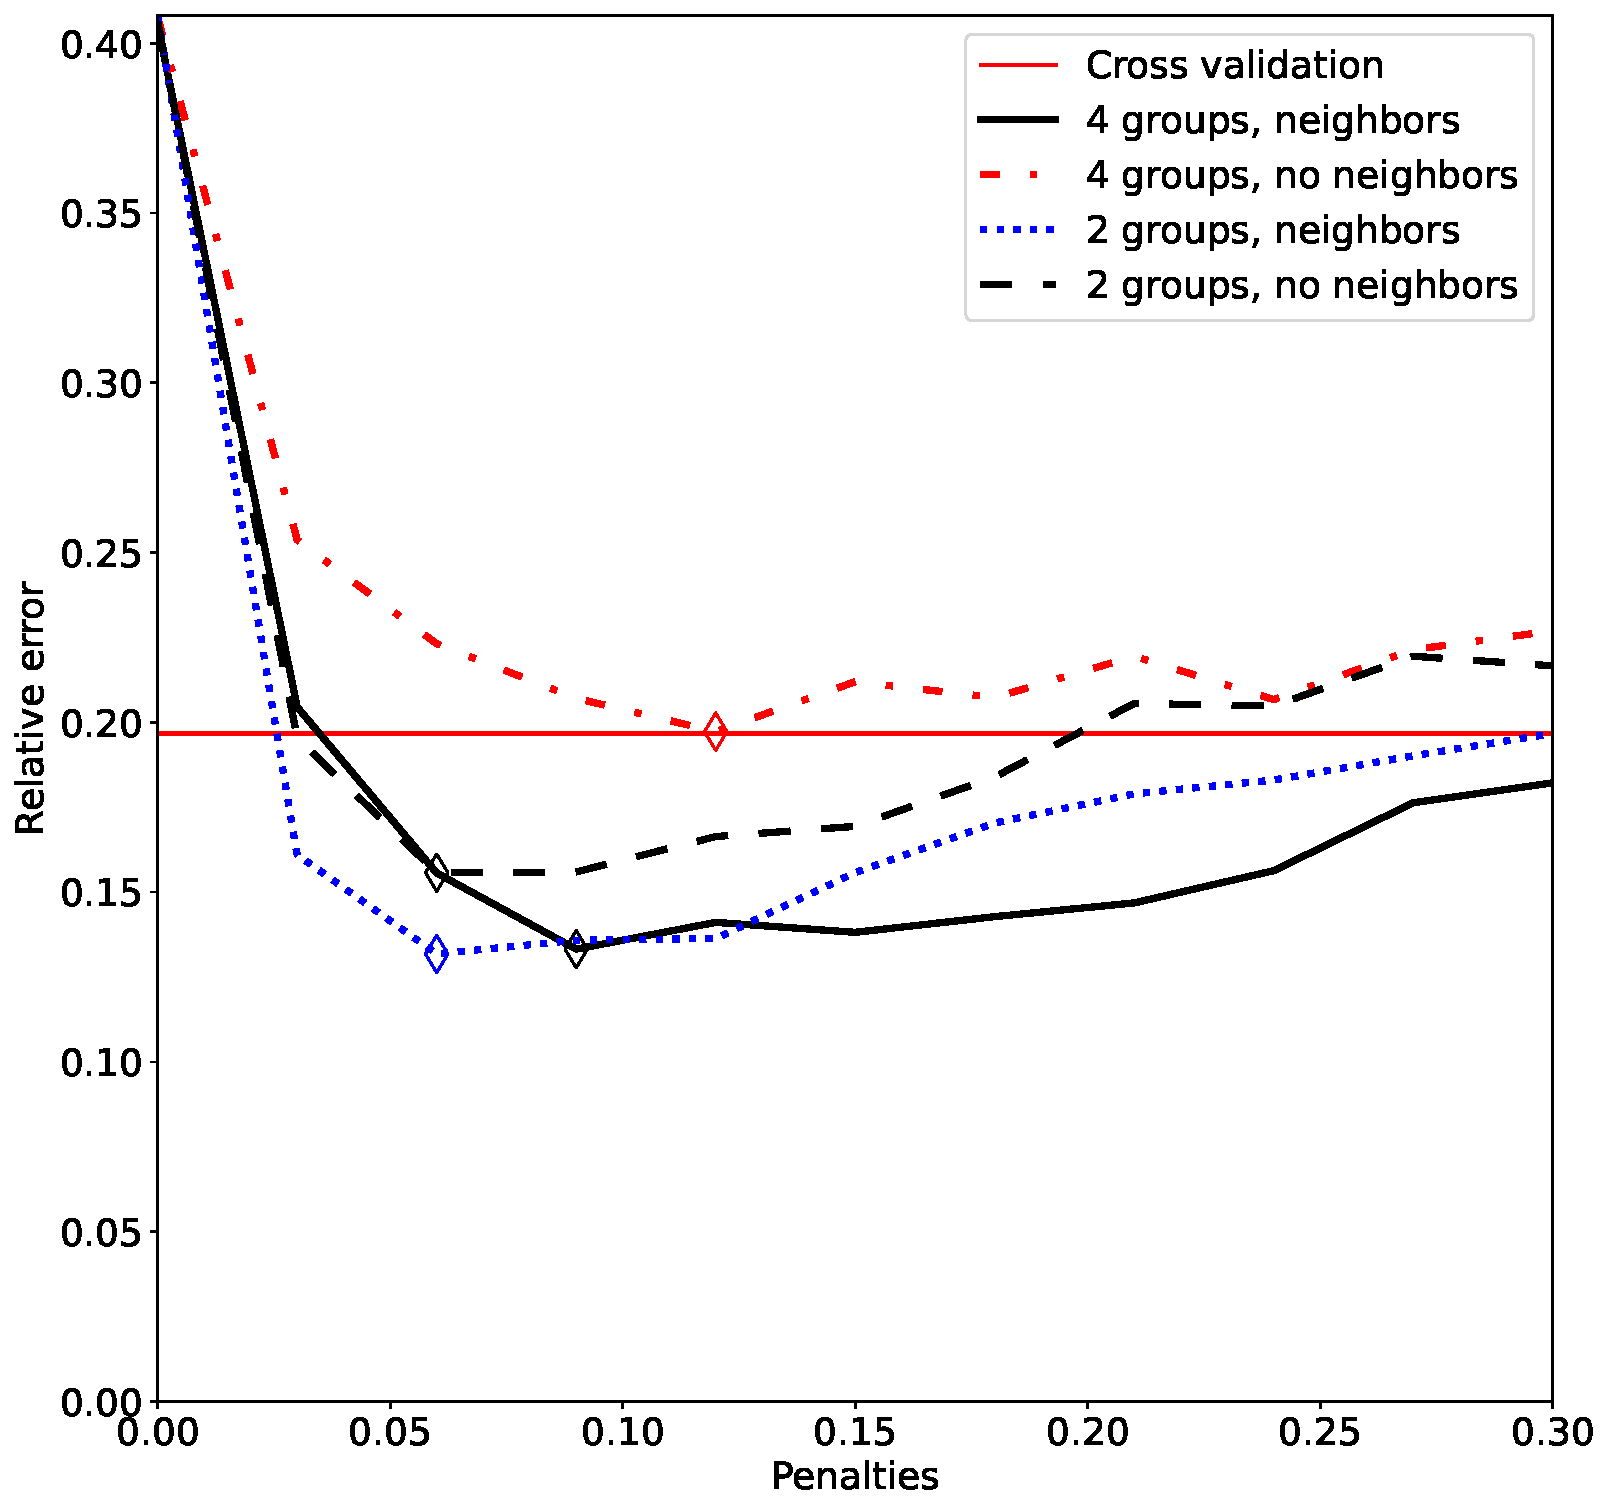
\includegraphics[scale=0.3]{20weeks_Color_Unknown_v3.pdf} \\
$\hspace*{0.6cm}$ $N_{i,t} = 14$ periods observed & $\hspace*{0.6cm}$ $N_{i,t} = 140$ periods observed
\vspace{5mm} \\
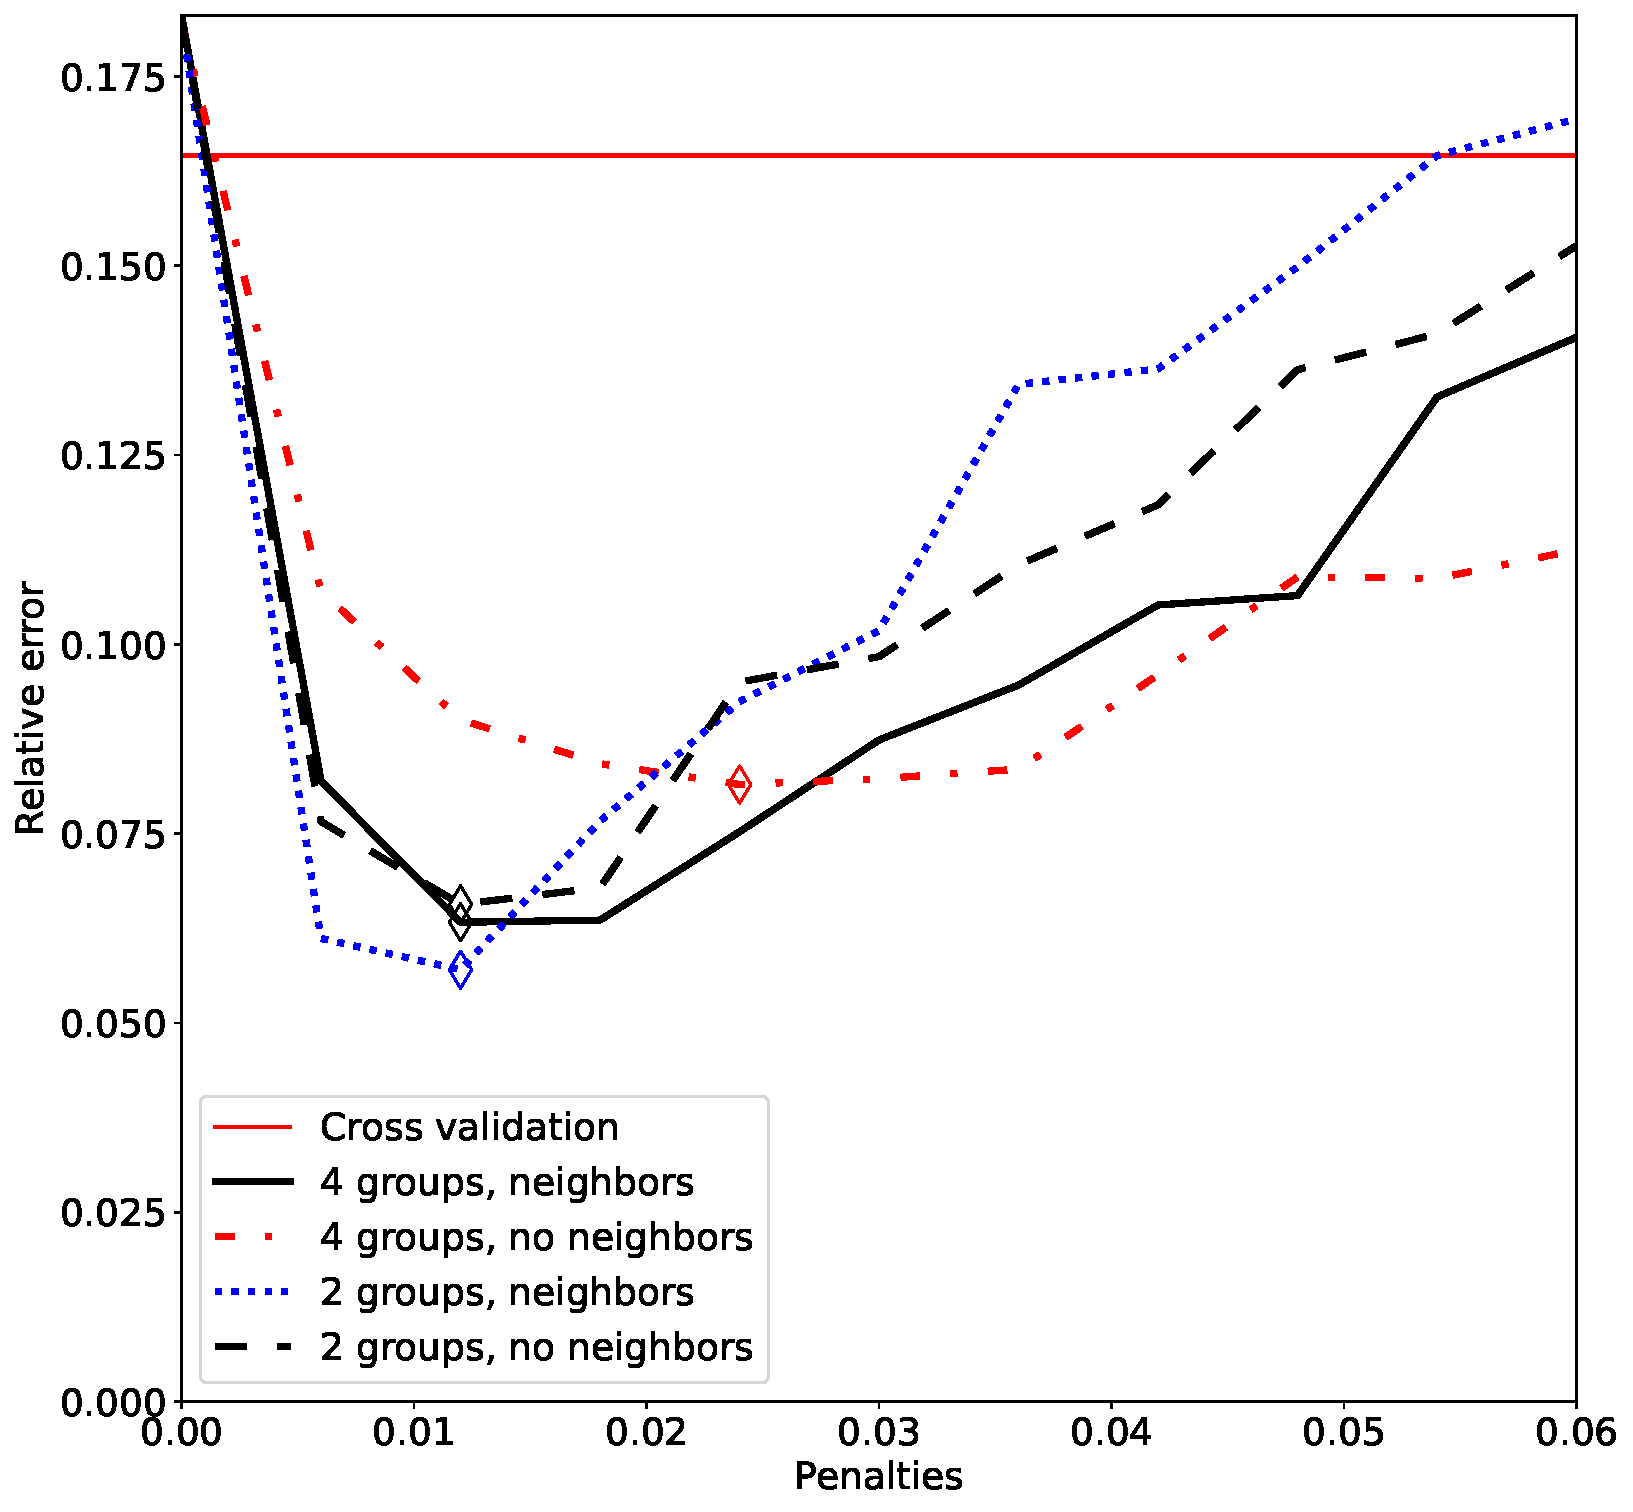
\includegraphics[scale=0.3]{100weeks_Color_Unknown_v3.pdf} &
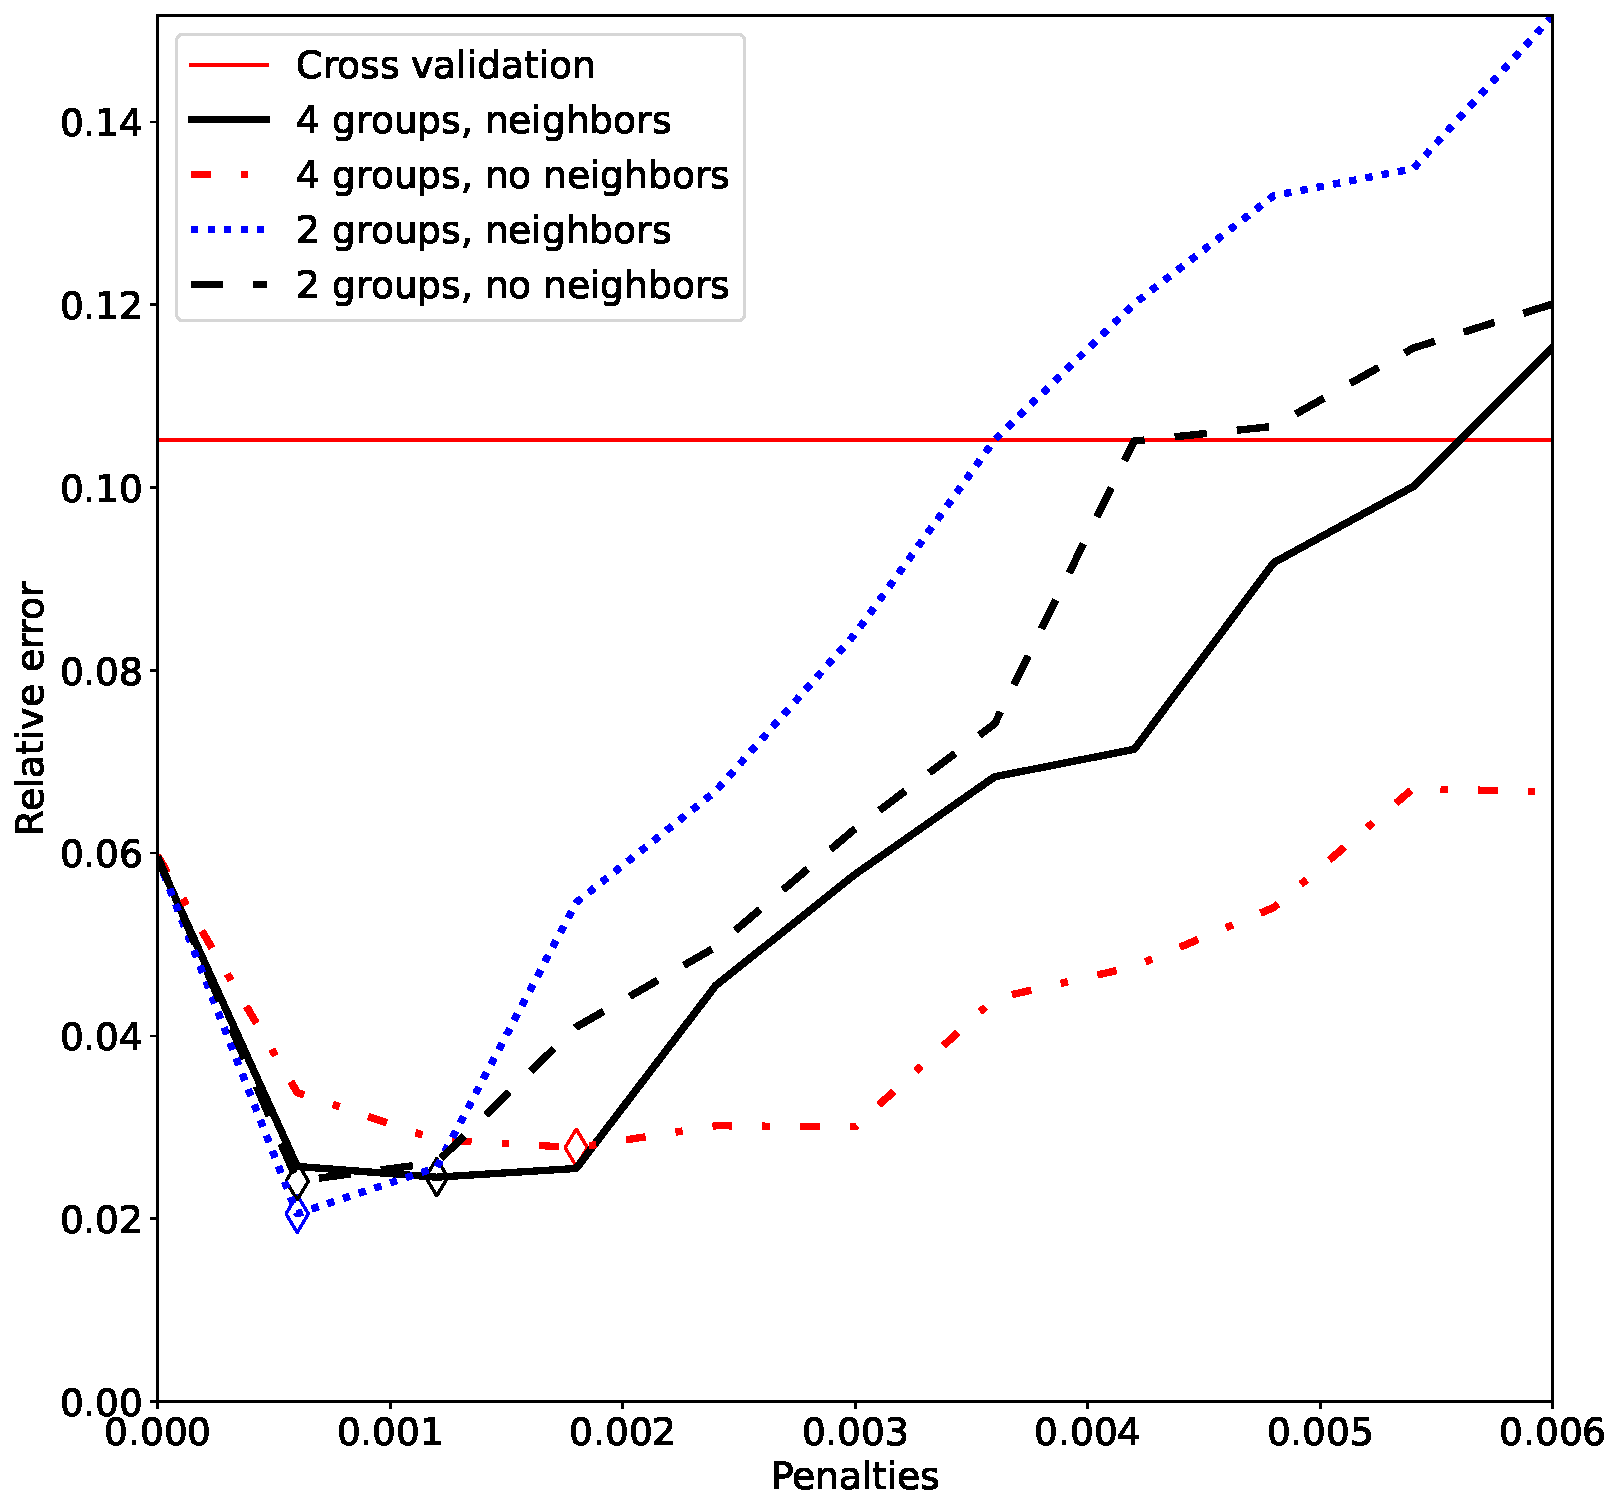
\includegraphics[scale=0.3]{1000weeks_Color_Unknown_v3.pdf}\\ 
$\hspace*{0.6cm}$ $N_{i,t} = 700$ periods observed \vspace{5mm} &
$\hspace*{0.6cm}$ $N_{i,t} = 7000$ periods observed \vspace{5mm}
\end{tabular}}
\caption{\label{figureserr1}
Mean relative estimation errors $\frac{1}{|\mathcal{I}||\mathcal{T}|} \sum_{i \in \mathcal{I}} \sum_{t \in \mathcal{T}} \left|\frac{\lambda_{i,t} - \hat{\lambda}^{w}_{i,t}}{\lambda_{i,t}}\right|$ as a function of the penalty parameter~$w$, for four sample sizes and six estimators (including the empirical estimator at $w = 0$).
%Intensities as in Figure~\ref{figuresex1}.
%where we take $p=w_{i,j}=W_G$ varying in the set $\{0$, $0.01$, $0.05$, $0.1$, $1$, $5$, $10$, $20$, $30$, $40$, $50$, $60$, $70$, $80$, $90$, $100$, $110$, $120$, $130$, $140$, $150$, $160$, $170$, $180$, $190$, $200$, $210$, $220$, $230$, $240$, $250$, $260$, $270$, $280$, $290$, $300$, $310$, $320$, $330$, $340$, $350$, $360$, $370$, $380$, $390$, $400\}$.
}
\end{figure}



In Figure~\ref{figureserr1}, note that the vertical and horizontal scales of the sub-figures are different.
As expected, the estimation error is decreasing in the sample size $N_{i,t}$.
Even when regularization is not based on the correct subregions and partition of time intervals, it can result in much better estimates than the empirical estimates (corresponding to $w = 0$), as long as reasonable values are chosen for~$w$.
Furthermore, note that the mean relative errors shown in Figure~\ref{figureserr1}, and the values of the penalty parameter~$w$ with the smallest mean relative errors (shown with diamonds), were based on using the correct values $\lambda_{i,t}$ in the calculations, which are not known by the user.
As explained before, we also used cross validation to determine good values of the penalty parameter~$w$ (without knowing the correct values $\lambda_{i,t}$), resulting in mean relative errors for most experiments much smaller than the mean relative error of the empirical estimator.

%Fourth, we see that the mean relative estimation error is a decreasing function of the penalty parameter for 100 and 1000 periods observed but for 2 and 20 periods observed the mean estimation error first tends to decrease until a penalty $\bar p$ and then tends to increase.
The results indicate that the improvement of the estimates using regularization is more pronounced when the number of observations is small: for $N_{i,t} = 14$, the estimation error decreases from about 120\% (for the empirical estimator) to about 29\% for the best regularized estimator, and for $N_{i,t} = 140$, the estimation error decreases from about 40\% to about 7\%.
Therefore, when a small amount of data are available, the regularized estimator results in a much smaller estimation error, even if the regularization is not based on the correct model structure, as long as relevant information is used for the regularization.
%Fifth, in general, the more (relevant) information is used, the better the estimator, meaning that the best regularized estimator is in general obtained taking 2 time groups and space regularization.

Figure~\ref{figureserrth} shows the true intensities $\lambda(s,t)$ and the estimates $\hat{\lambda}^{w^*}_{i,t}$ obtained with partition $\mathcal{G}_{2}$ of time intervals and with neighbor-based spatial regularization using the best penalty parameters~$w^*$, for $s \in \mathcal{R}$, zone $1 \in \mathcal{I}_{\mathcal{R}}$, $N_{i,t} = 14$ (top left plot), for $s \in \mathcal{R}$, zone $1 \in \mathcal{I}_{\mathcal{R}}$, $N_{i,t} = 140$ (bottom left plot), for $s \in \mathcal{B}$, zone $6 \in \mathcal{I}_{\mathcal{B}}$, $N_{i,t} = 14$ (top right plot), and for $s \in \mathcal{B}$, zone $6 \in \mathcal{I}_{\mathcal{B}}$, $N_{i,t} = 140$ (bottom right plot).
It can be seen that the regularized estimates are much closer to the true intensities than the empirical estimates.
%When a small number of observations is available (2 and 20 per zone for the experiment reported in Figure~\ref{figureserr2}), the empirical estimator's mean relative error can be large whereas the regularized estimator is already of good quality.


\begin{figure}
\centering
\resizebox{\textwidth}{!}{
%\scalebox{0.75}{
\begin{tabular}{cc}
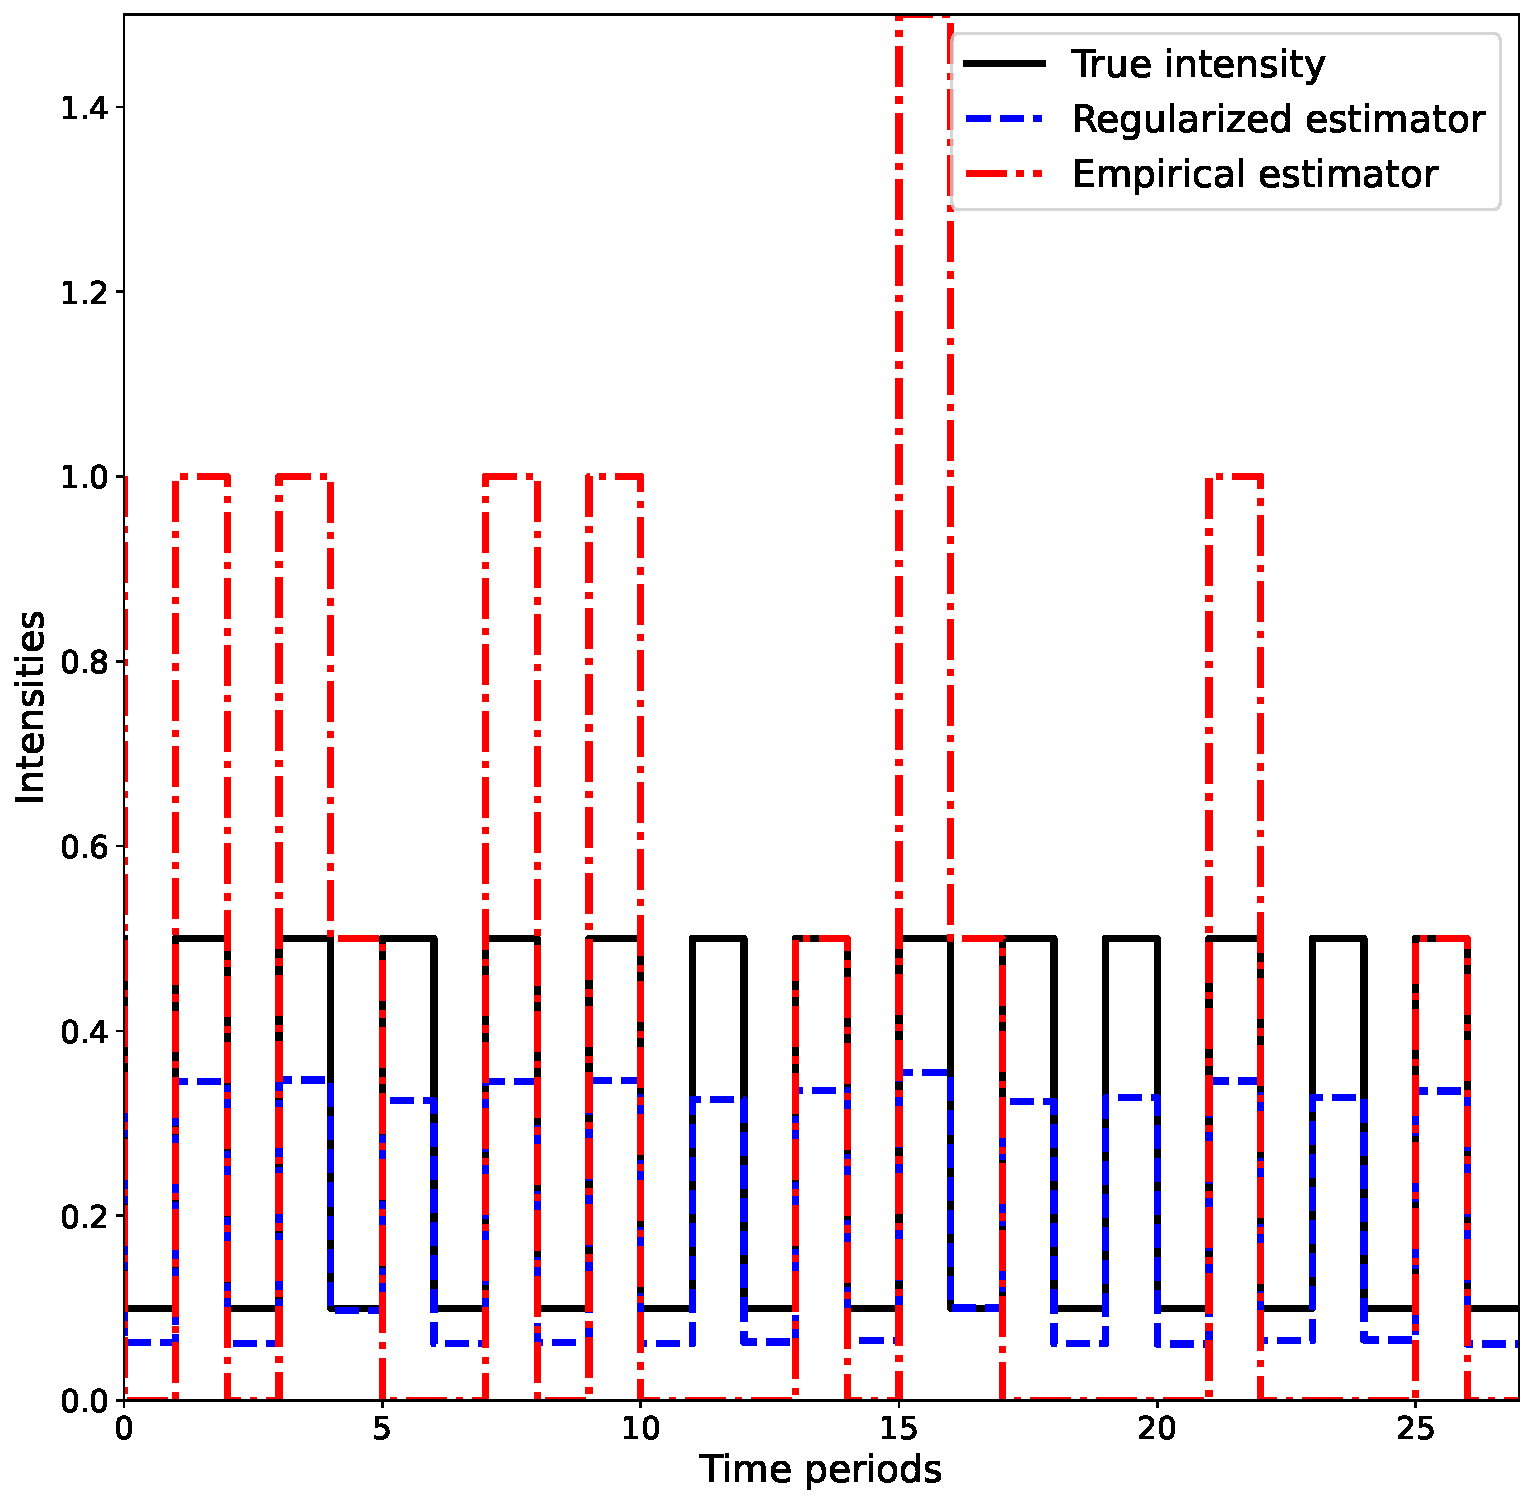
\includegraphics[scale=0.3]{rates2site1v3.pdf} &
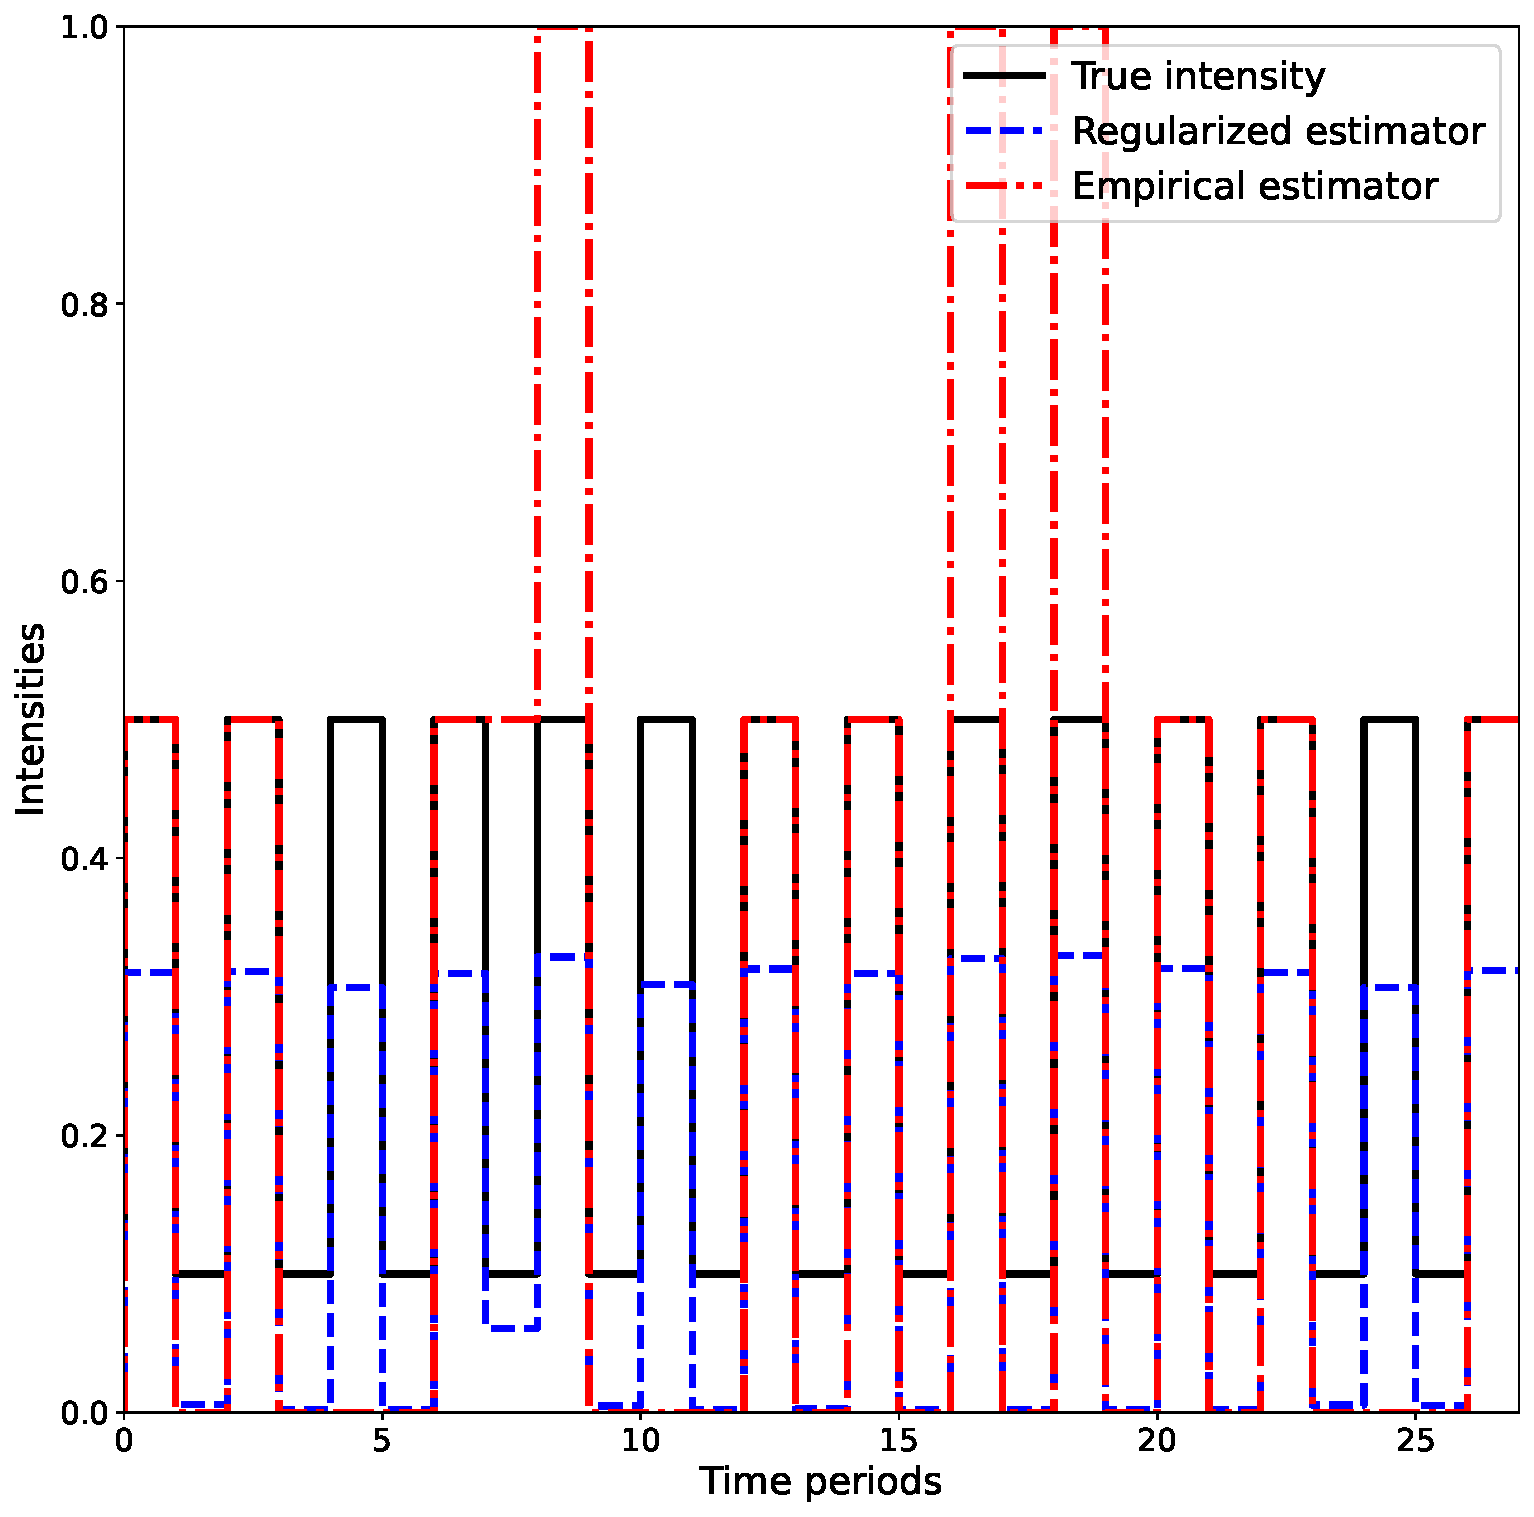
\includegraphics[scale=0.3]{rates2site6v3.pdf} \\
$\hspace*{0.6cm}$ $N_{i,t} = 14$, zone $1 \in \mathcal{I}_{\mathcal{R}}$ & $\hspace*{0.6cm}$ $N_{i,t} = 14
$, zone $6 \in \mathcal{I}_{\mathcal{B}}$
\vspace{5mm} \\
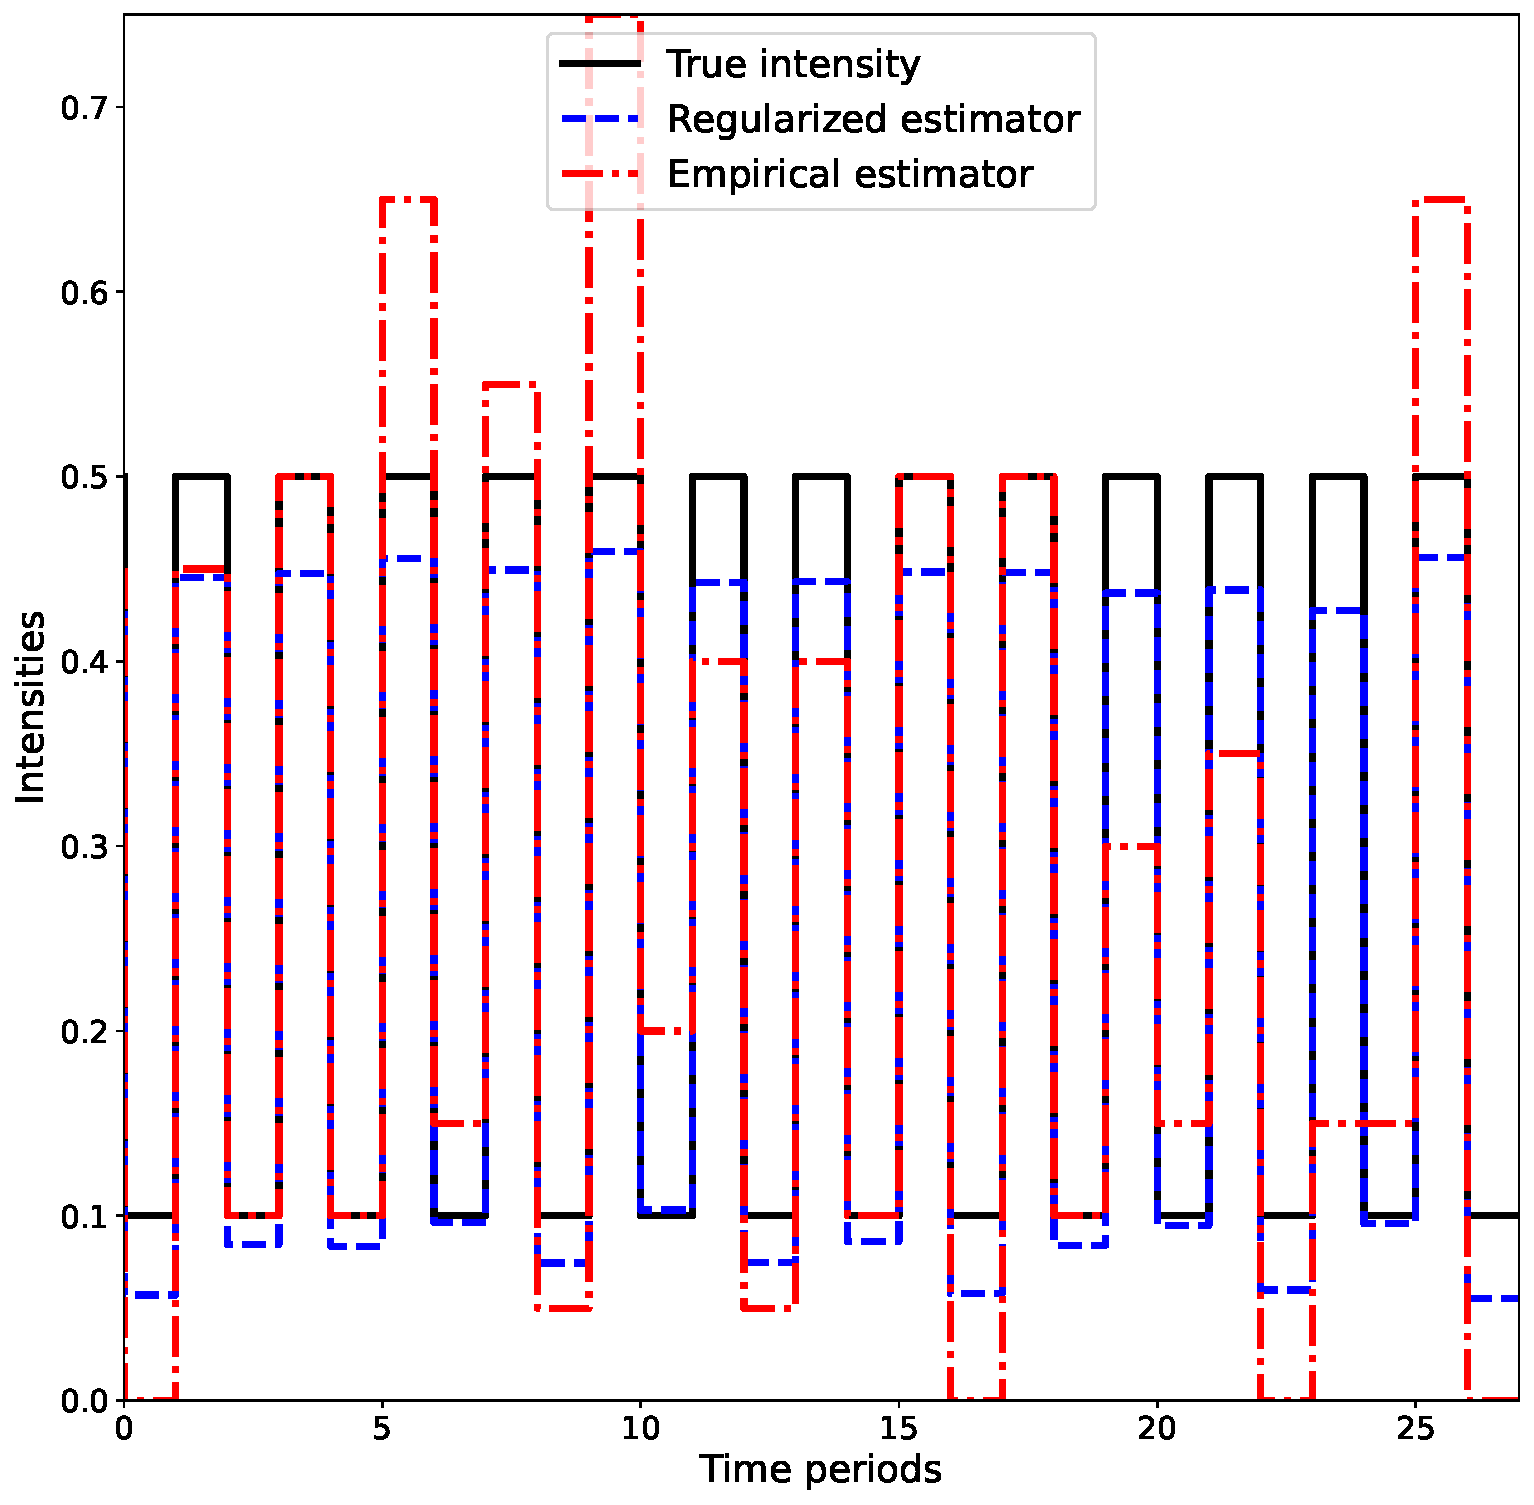
\includegraphics[scale=0.3]{rates20site1v3.pdf}&
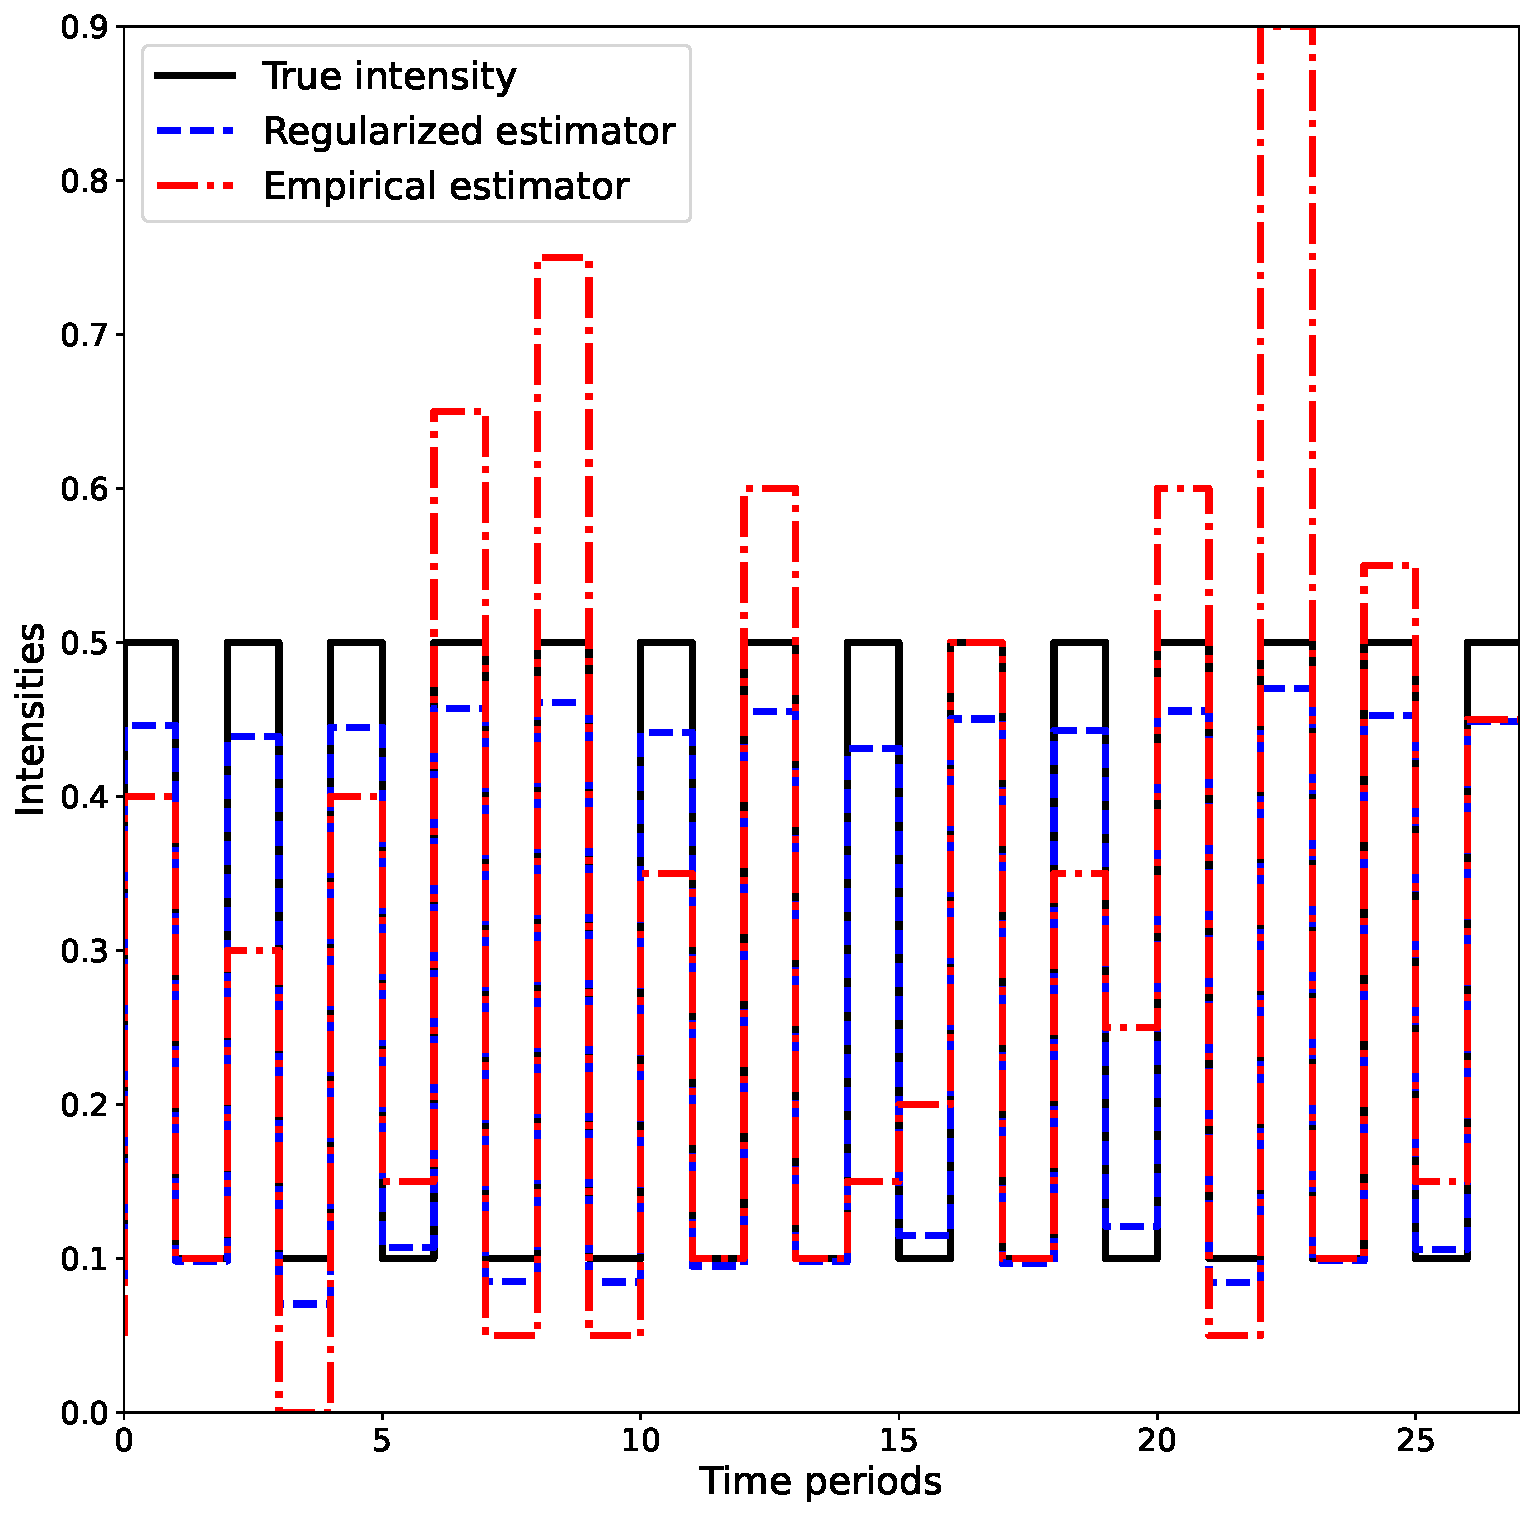
\includegraphics[scale=0.3]{rates20site6v3.pdf}\\
$\hspace*{0.6cm}$ $N_{i,t} = 140$, zone $1 \in \mathcal{I}_{\mathcal{R}}$ & $\hspace*{0.6cm}$ $N_{i,t} = 140$, zone $6 \in \mathcal{I}_{\mathcal{B}}$
\vspace{5mm}
\end{tabular}}
\caption{\label{figureserrth}
Comparison of true, empirical, and regularized estimates of the Poisson process intensities.
True intensities as shown in Figure~\ref{figuresex1}.}
\end{figure}


\subsubsection{Example~2}
\label{sec:example 2}

In this example, we consider the same region $\mathcal{S}$ and the same subregions $\mathcal{B}$ and $\mathcal{R}$ as in Example~1.
The intensity function $\lambda$ is also periodic, but not piecewise constant, as follows:
\[
\lambda(x,y,t) \ \ = \ \ \left\{
\begin{array}{lcl}
x + y & \mbox{if} & (x,y) \in \mathcal{B} \mbox{ and } t \in (2k,2k+1] \mbox{ for some } k \in \mathbb{N}, \\
5 (x + y) & \mbox{if} & (x,y) \in \mathcal{B} \mbox{ and } t \in (2k-1,2k] \mbox{ for some } k \in \mathbb{N}, \\
5 (x + y) & \mbox{if} & (x,y) \in \mathcal{R} \mbox{ and } t \in (2k,2k+1] \mbox{ for some } k \in \mathbb{N}, \\
x + y & \mbox{if} & (x,y) \in \mathcal{R} \mbox{ and } t \in (2k-1,2k] \mbox{ for some } k \in \mathbb{N}.
\end{array}\right.
\]
This rate function is represented in Figure~\ref{figuresex2}(c) (for time intervals that start at odd times) and Figure~\ref{figuresex2}(d) (for time intervals that start at even times). 

\begin{figure}
\centering
\resizebox{\textwidth}{!}{
%\scalebox{0.75}{
\begin{tabular}{cc}
\includegraphics[scale=0.6]{lambdanceven.pdf}&
\includegraphics[scale=0.6]{lambdancodd.pdf}\\
$\hspace*{0.6cm}$  (c) Time intervals that start at odd times& $\hspace*{0.6cm}$(d) Time intervals that start at even times
\end{tabular}}
\caption{\label{figuresex2}
Intensities as a function of location, for time intervals that start at odd times and even times.}
\end{figure}

As in Example~1, the user knows the region $\mathcal{S}$ and that $|\mathcal{C}| = 1$, but does not know about the subregions $\mathcal{B}$ and $\mathcal{R}$ that affect the intensity function $\lambda$, and does not know that $\lambda$ is periodic with period~$2$.
For estimation purposes, the user discretizes $\mathcal{S}$ into $100$~square zones of unit area each.
\if{

\noindent\rule[0.5ex]{1\columnwidth}{1pt}
{\textbf{Simulation of red and blue distributions for $t \in (2k-1,2k]$}}\\
    \noindent\rule[0.5ex]{1\columnwidth}{1pt}
$S_{\mathcal{B}}=\{\}, S_{\mathcal{R}}=\{\}$.\\
Generate $N_{t, \mathcal{B}}$ from the Poisson$(\Lambda_{t, \mathcal{B}})$ distribution. \\
Generate $N_{t, \mathcal{R}}$ from the Poisson$(\Lambda_{t, \mathcal{R}})$ distribution. \\
{\textbf{For }} $i = 1,\ldots,N_{t, \mathcal{B}}$ \\
\hspace*{0.8cm}ContBlue=1;\\
\hspace*{0.8cm}{\textbf{While }}ContBlue\\
\hspace*{2cm}Generate $(x,y)$ uniformly in $\mathcal{B}$. \\
\hspace*{2cm}Generate $U$ uniformly in $(0,\overline{\lambda}_{t, \mathcal{B}})$.\\
\hspace*{2cm}{\textbf{If }}$U \le \lambda(x,y,t)$, then\\ 
\hspace*{2.2cm}$S_{\mathcal{B}}=S_{\mathcal{B}} \cup \{(x,y)\}$, contBlue=0.\\
\hspace*{2cm}{\textbf{End If}}\\
\hspace*{0.8cm}{\textbf{End While}}\\
{\textbf{End For}}\\
{\textbf{For }} $i = 1,\ldots,N_{t, \mathcal{R}}$ \\
\hspace*{0.8cm}ContRed=1;\\
\hspace*{0.8cm}{\textbf{While }}ContRed\\
\hspace*{2cm}Generate $(x,y)$ uniformly in $\mathcal{R}$. \\
\hspace*{2cm}Generate $U$ uniformly in $(0,\overline{\lambda}_{t, \mathcal{R}})$.\\
\hspace*{2cm}{\textbf{If }}$U \le \lambda(x,y,t)$, then\\ 
\hspace*{2.2cm}$S_{\mathcal{R}}=S_{\mathcal{R}} \cup \{(x,y)\}$, contRed=0.\\
\hspace*{2cm}{\textbf{End If}}\\
\hspace*{0.8cm}{\textbf{End While}}\\
{\textbf{End For}}\\
\noindent\rule[0.5ex]{1\columnwidth}{1pt}

}\fi
The user computes the estimators $\hat{\lambda}^{w}_{i,t}$ for each $i \in \mathcal{I}$ and each $t \in \mathcal{T}$, by solving optimization problem~\eqref{eqn:reformmodel1} using regularization with penalty parameter~$w$ and $\varepsilon = 0.001$.
Each estimator $\hat{\lambda}^{w}_{i,t}$ now approximates the rate $\displaystyle \int_{R_{i}} \lambda(x,y,t) \diff(x,y)$, where $R_{i}$ denotes the square of unit area for zone~$i$.
For example, for a zone~$i$ with $R_{i} = (a_{i} - 1, a_{i}] \times (b_{j} - 1, b_{j}]$ and $\lambda(x,y,t) = x+y$ for $(x,y) \in R_{i}$, it holds that
\[
\int_{R_{i}} \lambda(x,y,t) \diff(x,y)
\ \ = \ \ \int_{a_{i} - 1}^{a_{i}} \int_{b_{j} - 1}^{b_{j}} (x+y) \diff x \diff y
\ \ = \ \ a_{i} + b_{j} - 1
\ \ = \ \ \lambda(x_{i},y_{i},t)
\ \ = \ \ x_{i} + y_{i}
\]
where $(x_{i},y_{i}) = (a_{i} - 0.5, b_{j} - 0.5)$ is the centroid of zone~$i$.

The mean relative error of estimator $\hat{\lambda}^{w}_{i,t}$ is now given by
\[
\frac{1}{|\mathcal{I}| |\mathcal{T}|} \sum_{i \in \mathcal{I}} \sum_{t \in \mathcal{T}} \frac{\left|\displaystyle \int_{R_{i}} \lambda(x,y,t) \diff(x,y) - \hat{\lambda}^{w}_{i,t}\right|}{\displaystyle \int_{R_{i}} \lambda(x,y,t) \diff(x,y)}
\ \ = \ \ \frac{1}{|\mathcal{I}| |\mathcal{T}|} \sum_{i \in \mathcal{I}} \sum_{t \in \mathcal{T}} \frac{\left|\lambda(x_{i},y_{i},t) - \hat{\lambda}^{w}_{i,t}\right|}{\lambda(x_{i},y_{i},t)}.
\]
Parameter estimates $\hat{\lambda}^{w}_{i,t}$ were computed for a range of values of the penalty parameter~$w$, for the same four estimators as in Example~1: estimator with partition $\mathcal{G}_{4}$ of time intervals and with neighbor-based spatial regularization (legend ``4 groups, neighbors'' in Figure~\ref{figureserr2pl}), estimator with partition $\mathcal{G}_{4}$ of time intervals and without spatial regularization (legend ``4 groups, no neighbors'' in Figure~\ref{figureserr2pl}), estimator with partition $\mathcal{G}_{2}$ of time intervals and with neighbor-based spatial regularization (legend ``2 groups, neighbors'' in Figure~\ref{figureserr2pl}), and estimator with partition $\mathcal{G}_{2}$ of time intervals and without spatial regularization (legend ``2 groups, no neighbors'' in Figure \ref{figureserr2pl}).
As before, four values were used for the sample size: $N_{i,t} = 14$, $N_{i,t} = 140$, $N_{i,t} = 700$, and $N_{i,t} = 7000$.
Figure~\ref{figureserr2pl} shows the mean relative error for these four estimators, as well as the estimator with partition $\mathcal{G}_{2}$ of time intervals and with neighbor-based spatial regularization using the penalty parameter~$w^*$ chosen with cross validation.
As before, the empirical estimator corresponds to~$w = 0$.
%For this experiment, relative errors started to decrease until some penalty $w_*$ and then to increase with a high rate for all estimators, where $w_*$ depends on the estimator and on the number of observations.
%We only represented the values of the relative errors for $w \in [0,\hat{w}]$, where $\hat{w}$ was chosen as a penalty slightly above $w_*$ to observe on the figure values of penalties giving estimators better than the empirical estimator.
%For this problem, the regularized estimators are better than the empirical estimator for all 4 sample sizes and some well chosen values of penalties.
%In this example, the mean relative errors are more sensitive regarding penalty parameter~$w$ than in Example~1 with piecewise constant intensities.
%For small sample sizes, for some well-chosen penalties the regularized estimator mean relative error is smaller than the empirical mean relative error, whereas for large sample sizes, the empirical estimator is better than any other regularized estimator.
%This makes sense since regularization helps to compensate for the lack of data using appropriate, relevant information.

%Moreover, estimators with 2 time groups perform in general better than estimators using 4 time groups, which makes sense since we expect to get better estimators when more relevant information is used.


\begin{figure}
\centering
\resizebox{\textwidth}{!}{
%\scalebox{0.75}{
\begin{tabular}{cc}
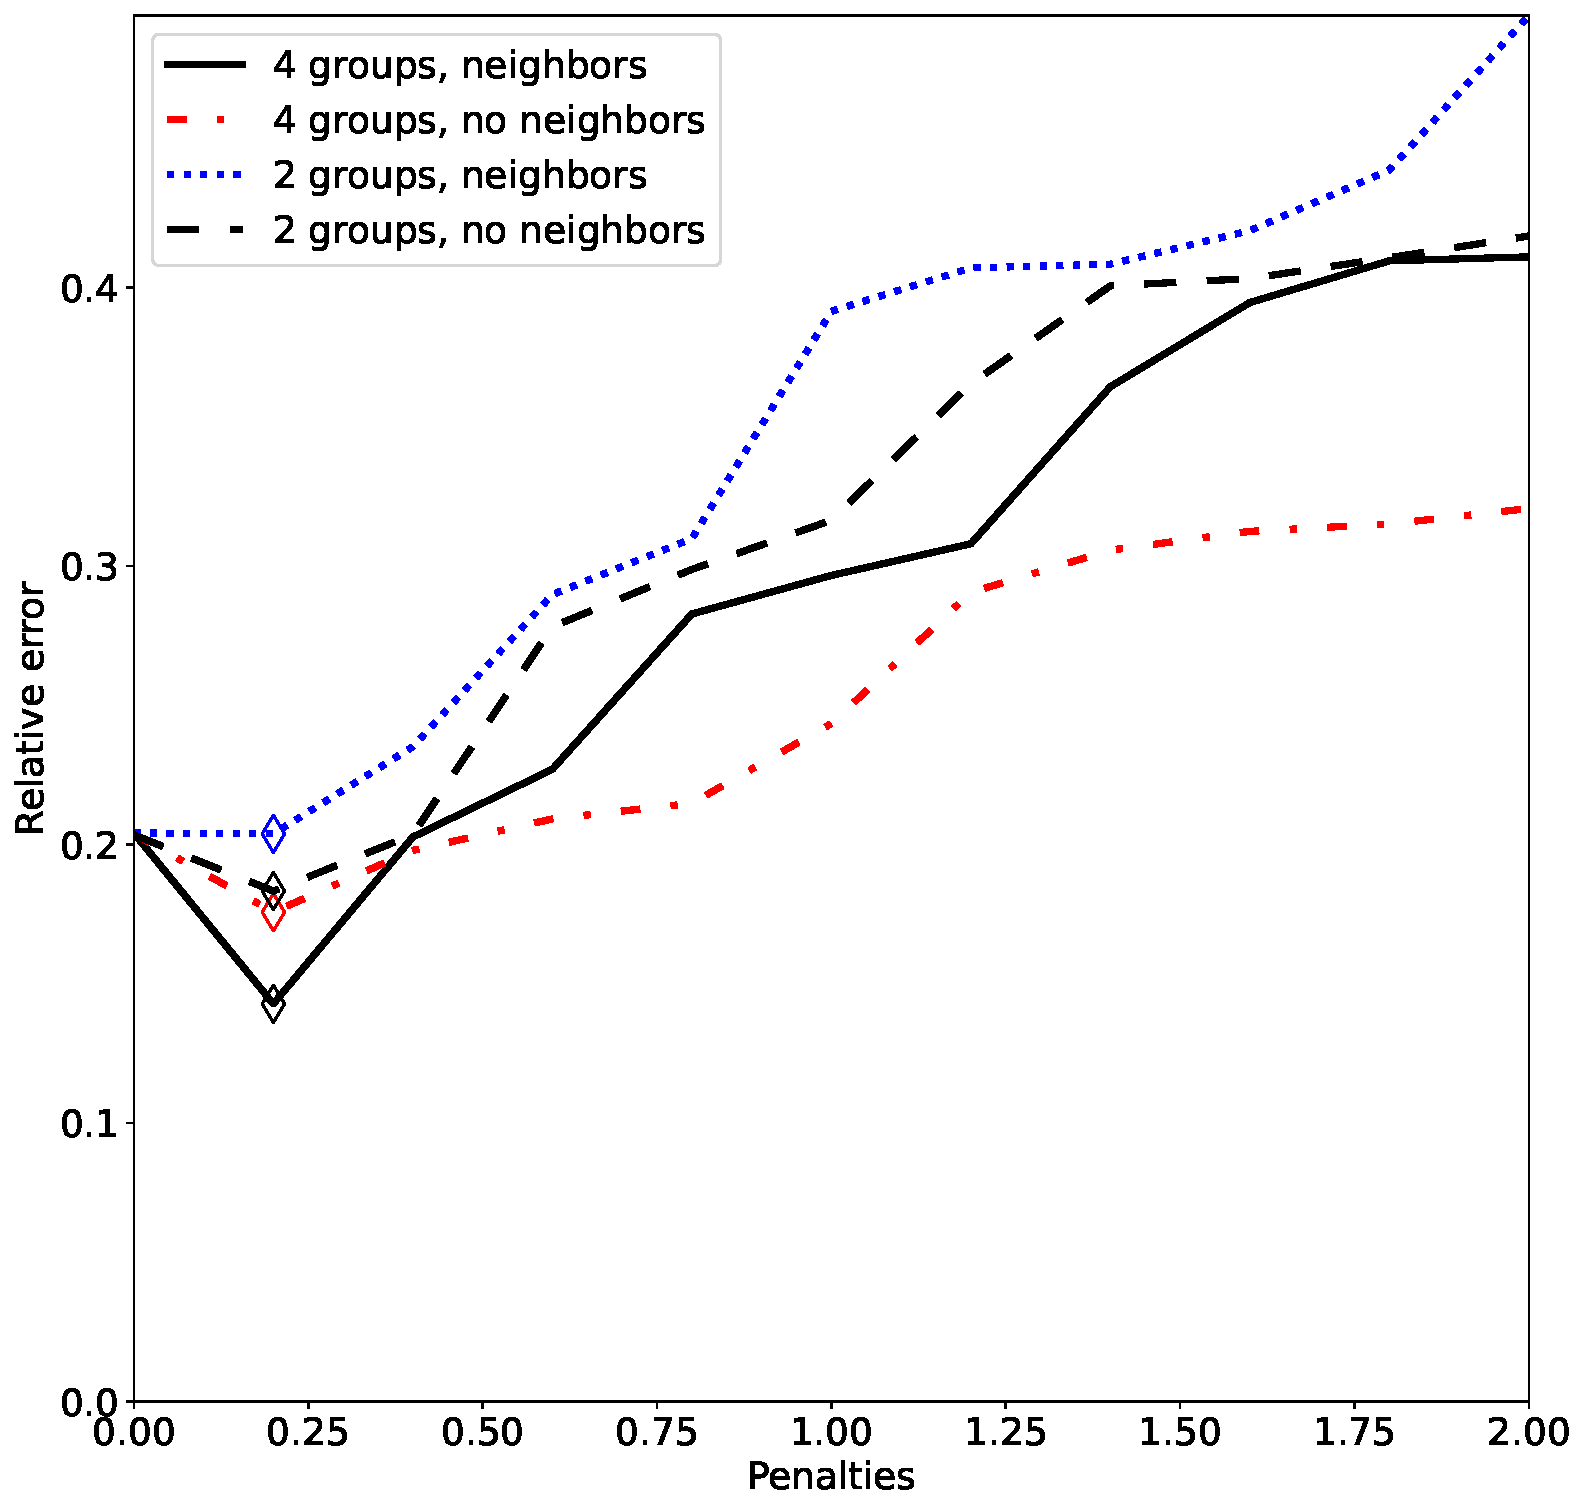
\includegraphics[scale=0.3]{2weeks_Color_Unknown_v3_model2.pdf} &
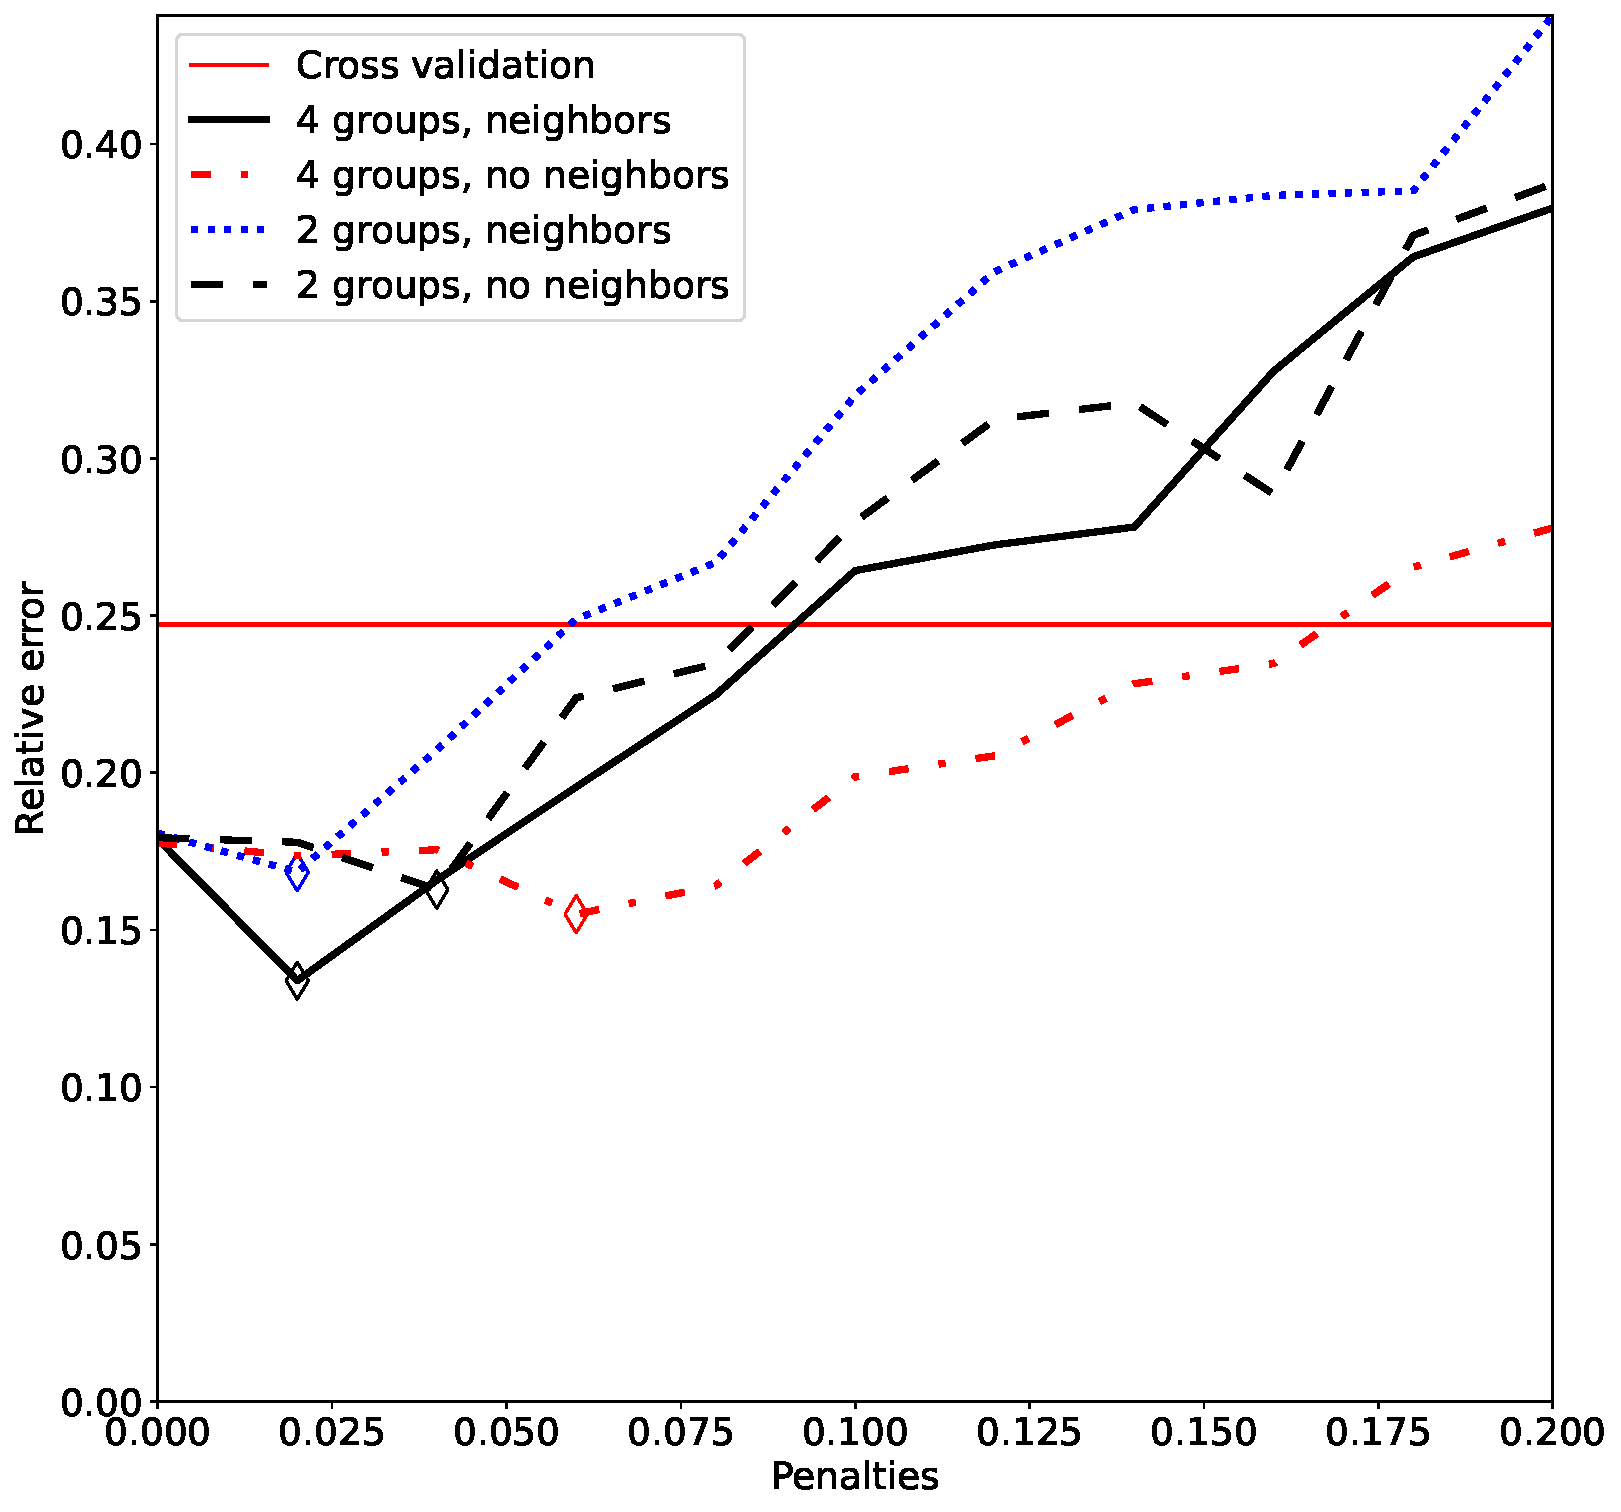
\includegraphics[scale=0.3]{20weeks_Color_Unknown_v3_model2.pdf} \\
$\hspace*{0.6cm}$ $N_{i,t} = 14$ periods observed & $\hspace*{0.6cm}$ $N_{i,t} = 140$ periods observed
\vspace{5mm} \\
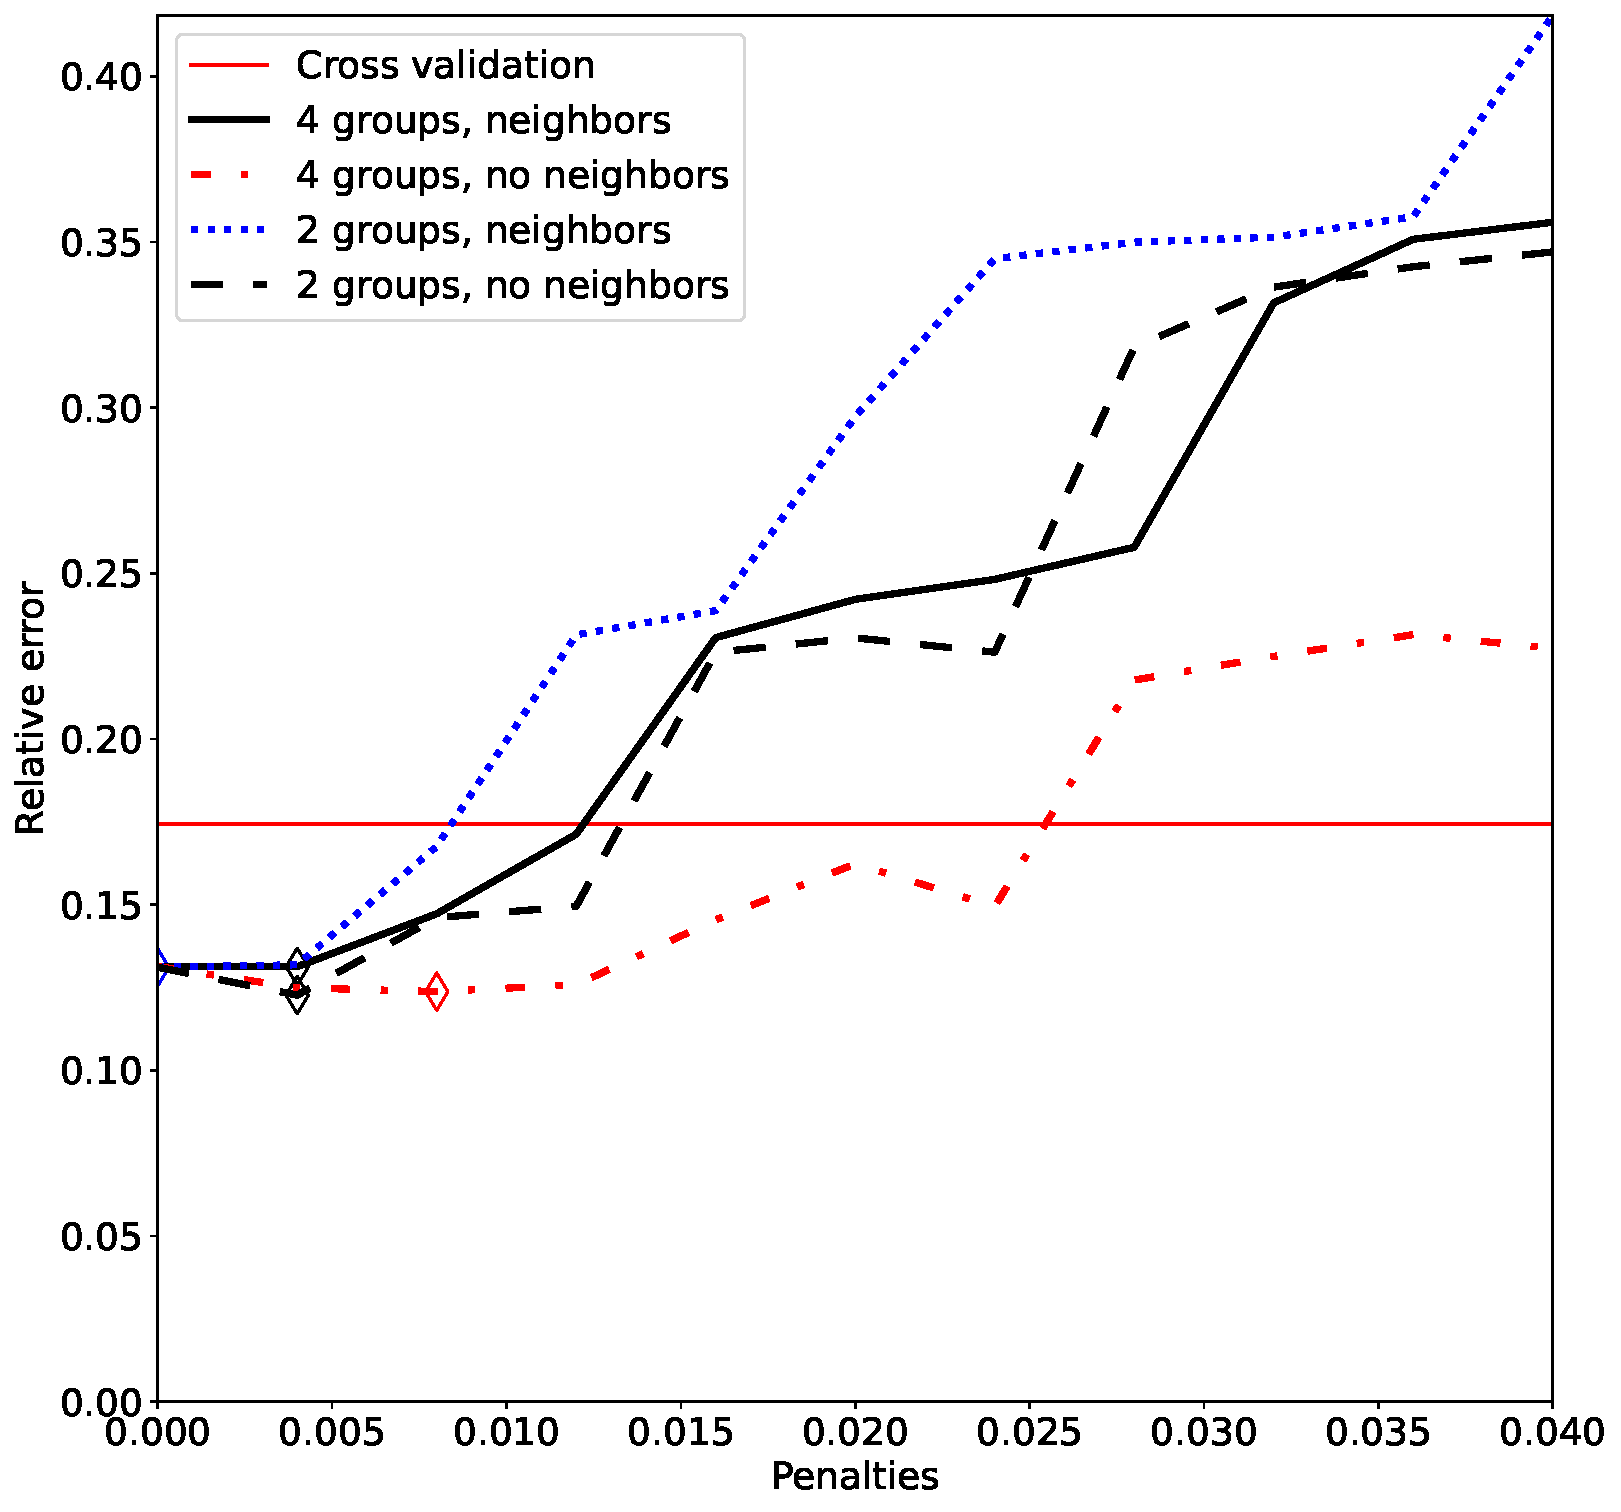
\includegraphics[scale=0.3]{100weeks_Color_Unknown_v3_model2.pdf} &
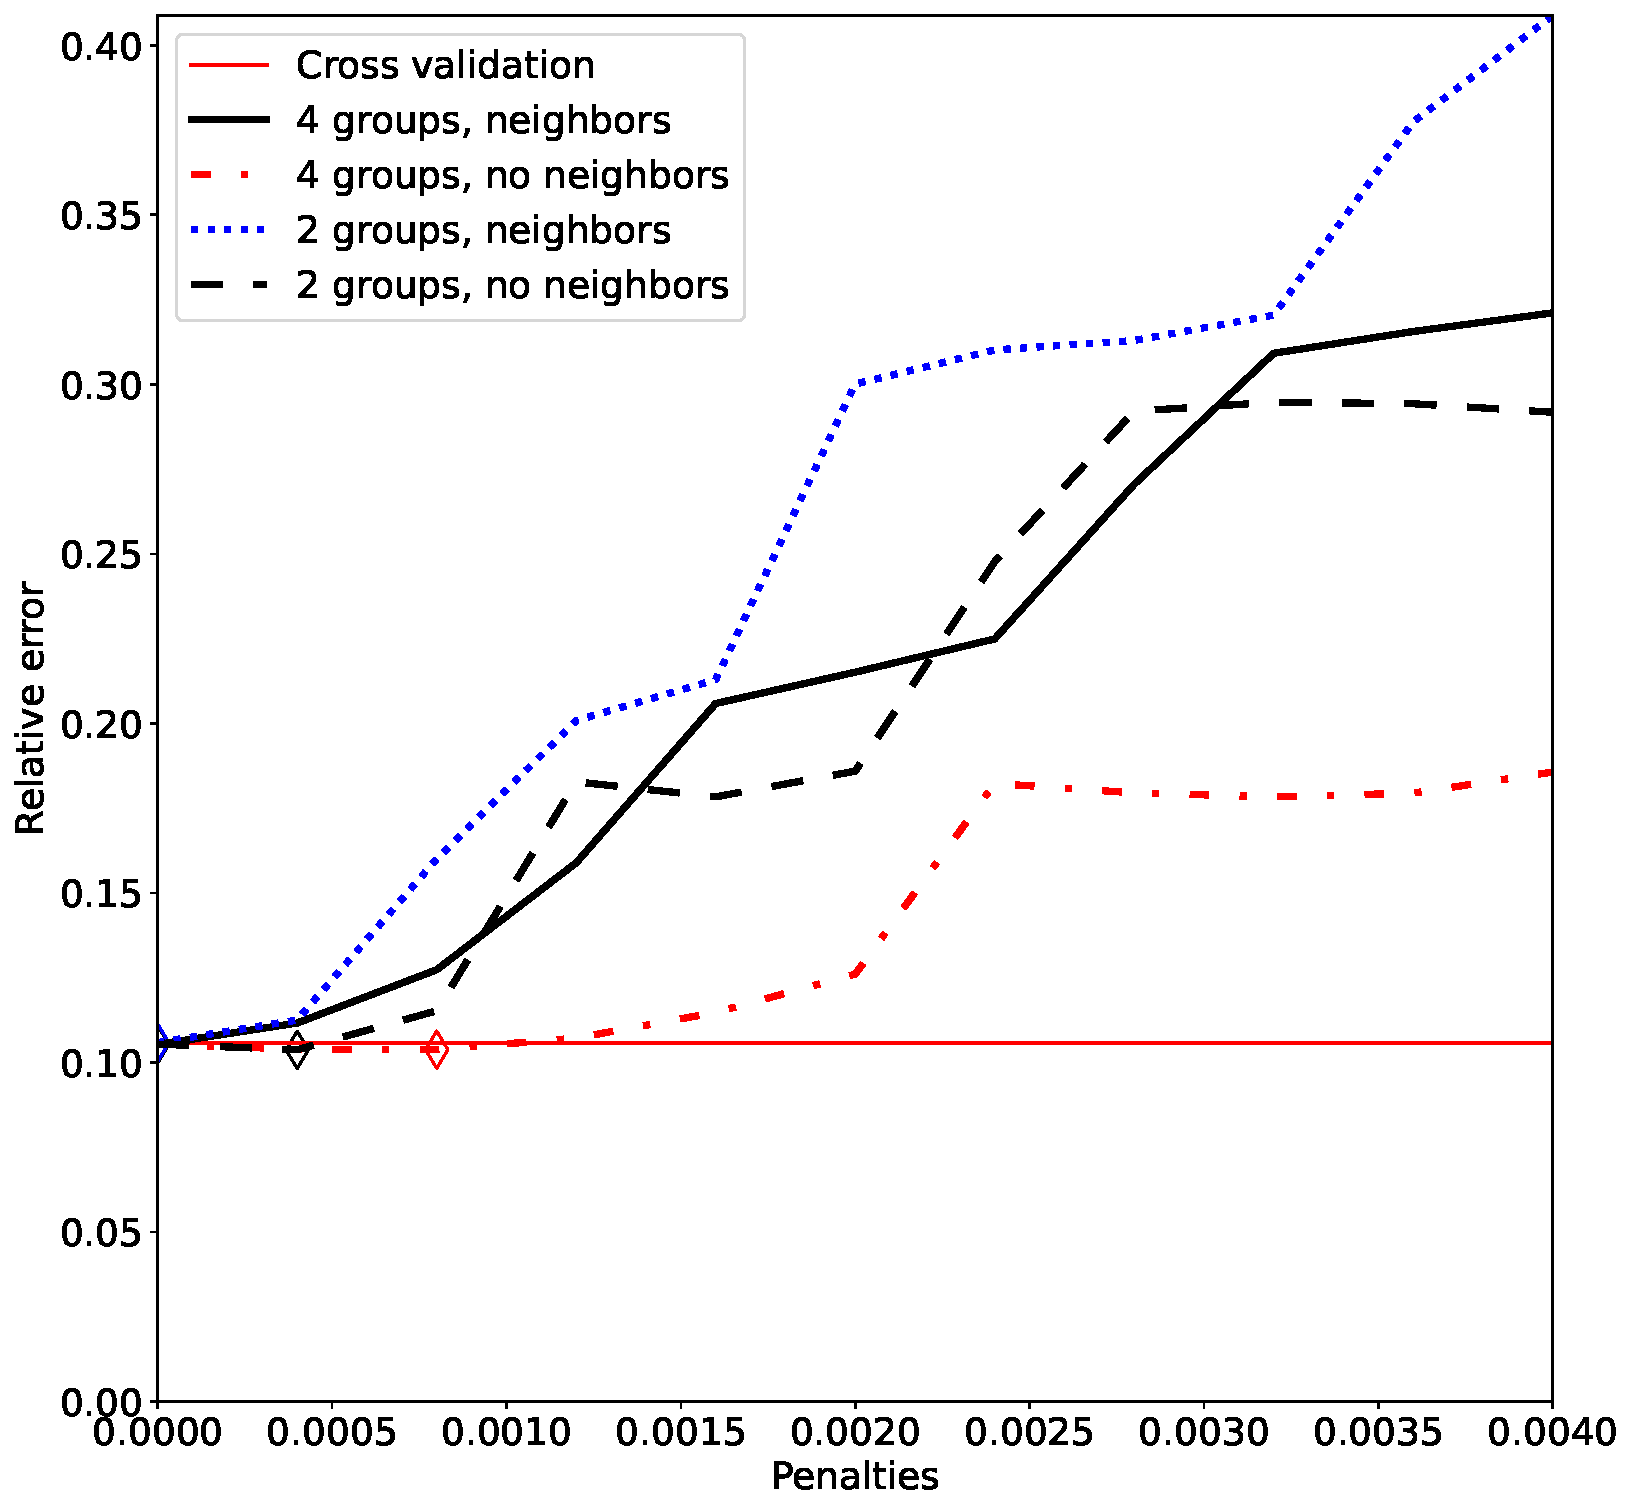
\includegraphics[scale=0.3]{1000weeks_Color_Unknown_v3_model2.pdf} \\
$\hspace*{0.6cm}$ $N_{i,t} = 700$ periods observed & $\hspace*{0.6cm}$ $N_{i,t} = 7000$ periods observed
\end{tabular}}
\caption{\label{figureserr2pl}
Mean relative errors $\frac{1}{|\mathcal{I}| |\mathcal{T}|}   \displaystyle \sum_{t \in \mathcal{T}} \sum_{i \in \mathcal{I}} \frac{\left|\displaystyle \int_{R_i} \lambda(x,y,t)d(x,y)-{\hat \lambda}_{t,i}^{w}\right|}{\displaystyle \int_{R_i} \lambda(x,y,t)d(x,y)}$
as a function of the penalty parameter~$w$. Intensities as in Figure
\ref{figuresex2}.
%where we take $p=w_{i,j}=W_G$ varying in the set $\{0$, $0.01$, $0.05$, $0.1$, $1$, $5$, $10$, $20$, $30$, $40$, $50$, $60$, $70$, $80$, $90$, $100$, $110$, $120$, $130$, $140$, $150$, $160$, $170$, $180$, $190$, $200$, $210$, $220$, $230$, $240$, $250$, $260$, $270$, $280$, $290$, $300$, $310$, $320$, $330$, $340$, $350$, $360$, $370$, $380$, $390$, $400\}$.
}
\end{figure}


% \begin{figure}
% \centering
% \begin{tabular}{cc}
% \includegraphics[scale=0.6]{contlambda2v2.pdf} &
% \includegraphics[scale=0.6]{contlambda20v2.pdf} \\
% $\hspace*{0.6cm}$ $N_{i,t} = 14$ periods observed & $\hspace*{0.6cm}$ $N_{i,t} = 140$ periods observed
% \vspace{5mm} \\
% \includegraphics[scale=0.6]{contlambda100v2.pdf} &
% \includegraphics[scale=0.6]{contlambda1000v2.pdf} \\
% $\hspace*{0.6cm}$ $N_{i,t} = 700$ periods observed & $\hspace*{0.6cm}$ $N_{i,t} = 7000$ periods observed
% \end{tabular}
% \caption{\label{figureserr2pl}
% Mean relative errors $\frac{1}{|\mathcal{I}| |\mathcal{T}|}   \displaystyle \sum_{t \in \mathcal{T}} \sum_{i \in \mathcal{I}} \frac{\left|\displaystyle \int_{R_i} \lambda(x,y,t)d(x,y)-{\hat \lambda}_{t,i}^{w}\right|}{\displaystyle \int_{R_i} \lambda(x,y,t)d(x,y)}$
% as a function of the penalty parameter~$w$. Intensities as in Figure
% \ref{figuresex2}.
% %where we take $p=w_{i,j}=W_G$ varying in the set $\{0$, $0.01$, $0.05$, $0.1$, $1$, $5$, $10$, $20$, $30$, $40$, $50$, $60$, $70$, $80$, $90$, $100$, $110$, $120$, $130$, $140$, $150$, $160$, $170$, $180$, $190$, $200$, $210$, $220$, $230$, $240$, $250$, $260$, $270$, $280$, $290$, $300$, $310$, $320$, $330$, $340$, $350$, $360$, $370$, $380$, $390$, $400\}$.
% }
% \end{figure}

\if{
\begin{figure}
\centering
\begin{tabular}{cc}
\includegraphics[scale=0.3]{results_cov_n2_crop.pdf} &
\includegraphics[scale=0.3]{results_cov_n20_crop.pdf} \\
$\hspace*{0.6cm}$ $N_{i,t} = 14$ periods observed & $\hspace*{0.6cm}$ $N_{i,t} = 140$ periods observed
\vspace{5mm} \\
\includegraphics[scale=0.3]{results_cov_n100_crop.pdf} &
\includegraphics[scale=0.3]{results_cov_n1000_crop.pdf} \\
$\hspace*{0.6cm}$ $N_{i,t} = 700$ periods observed & $\hspace*{0.6cm}$ $N_{i,t} = 7000$ periods observed
\end{tabular}
\caption{\label{figureserr2pl}
Relative estimation  errors for covariates without holidays. The horizontal line denotes the relative error for the model with regressors. \(N1\) considers each zone has eight neighbors and only apply penalties if neighboring zones are of the same color. \(N2\) considers each zone only has four neighbors and apply penalties regardless of color.
%where we take $p=w_{i,j}=W_G$ varying in the set $\{0$, $0.01$, $0.05$, $0.1$, $1$, $5$, $10$, $20$, $30$, $40$, $50$, $60$, $70$, $80$, $90$, $100$, $110$, $120$, $130$, $140$, $150$, $160$, $170$, $180$, $190$, $200$, $210$, $220$, $230$, $240$, $250$, $260$, $270$, $280$, $290$, $300$, $310$, $320$, $330$, $340$, $350$, $360$, $370$, $380$, $390$, $400\}$.
}
\end{figure}

\begin{figure}
\centering
\begin{tabular}{cc}
\includegraphics[scale=0.3]{results_covh_n2_crop.pdf} &
\includegraphics[scale=0.3]{results_covh_n20_crop.pdf} \\
$\hspace*{0.6cm}$ $N_{i,t} = 14$ periods observed & $\hspace*{0.6cm}$ $N_{i,t} = 140$ periods observed
\vspace{5mm} \\
\includegraphics[scale=0.3]{results_covh_n100_crop.pdf} &
\includegraphics[scale=0.3]{results_covh_n1000_crop.pdf} \\
$\hspace*{0.6cm}$ $N_{i,t} = 700$ periods observed & $\hspace*{0.6cm}$ $N_{i,t} = 7000$ periods observed
\end{tabular}
\caption{\label{figureserr2pl}
Relative estimation errors for covariates with holidays. The horizontal line denotes the relative error for the model with regressors. \(N1\) considers each zone has eight neighbors and only apply penalties if neighboring zones are of the same color. \(N2\) considers each zone only has four neighbors and apply penalties regardless of color.
%where we take $p=w_{i,j}=W_G$ varying in the set $\{0$, $0.01$, $0.05$, $0.1$, $1$, $5$, $10$, $20$, $30$, $40$, $50$, $60$, $70$, $80$, $90$, $100$, $110$, $120$, $130$, $140$, $150$, $160$, $170$, $180$, $190$, $200$, $210$, $220$, $230$, $240$, $250$, $260$, $270$, $280$, $290$, $300$, $310$, $320$, $330$, $340$, $350$, $360$, $370$, $380$, $390$, $400\}$.
}
\end{figure}


\begin{figure}
\centering
\begin{tabular}{cc}
\includegraphics[scale=0.3]{results_clam_n2_crop.pdf} &
\includegraphics[scale=0.3]{results_clam_n20_crop.pdf} \\
$\hspace*{0.6cm}$ $N_{i,t} = 14$ periods observed & $\hspace*{0.6cm}$ $N_{i,t} = 140$ periods observed
\vspace{5mm} \\
\includegraphics[scale=0.3]{results_clam_n100_crop.pdf} &
\includegraphics[scale=0.3]{results_clam_n1000_crop.pdf} \\
$\hspace*{0.6cm}$ $N_{i,t} = 700$ periods observed & $\hspace*{0.6cm}$ $N_{i,t} = 7000$ periods observed
\end{tabular}
\caption{\label{figureserr2pl}
Relative estimation  errors for parameters according to figure~\ref{figuresex2}. \(N1\) considers each zone has eight neighbors and only apply penalties if neighboring zones are of the same color. \(N2\) considers each zone only has four neighbors and apply penalties regardless of color.
%where we take $p=w_{i,j}=W_G$ varying in the set $\{0$, $0.01$, $0.05$, $0.1$, $1$, $5$, $10$, $20$, $30$, $40$, $50$, $60$, $70$, $80$, $90$, $100$, $110$, $120$, $130$, $140$, $150$, $160$, $170$, $180$, $190$, $200$, $210$, $220$, $230$, $240$, $250$, $260$, $270$, $280$, $290$, $300$, $310$, $320$, $330$, $340$, $350$, $360$, $370$, $380$, $390$, $400\}$.
}
\end{figure}

}\fi


\subsection{Numerical Example with Artificial Data with Covariates}

As in the previous examples, points arrive in $\mathcal{S} = [0,10]^2$ and over time according to a periodic nonhomogeneous Poisson process.
Region $\mathcal{S}$ is partitioned into two subregions $\mathcal{S} = \mathcal{B} \cup \mathcal{R}$, with $\mathcal{B} = [0,5] \times (5,10] \cup (5,10] \times [0,5]$ and $\mathcal{R} = [0,5] \times [0,5] \cup (5,10] \times (5,10]$.
There is only one type of point, thus $|\mathcal{C}| = 1$, and hence the type notation~$c$ is omitted.
%The region under consideration is $\mathcal{S} = [0,10]^2$, as shown in Figure~\ref{figureserr}.
Each point $s \in \mathcal{S}$ has three attributes, denoted $x(s) \defi (x_{1}(s),x_{2}(s),x_{3}(s))$.
For example, $x_{1}(s)$ denotes the population density at location~$s$, $x_{2}(s) = 1$ if the land at location~$s$ is used for commerce and $x_{2}(s) = 0$ otherwise, and $x_{3}(s) = 1$ if the land at location~$s$ is used for manufacturing and $x_{3}(s) = 0$ otherwise.

For the examples, $x(s)$ was generated as follows.
Let $U^{b}_{j}$, $U^{r}_{j}$, $j = 1,\ldots, 20$, be independent random variables uniformly distributed on $(0,1)$.
For $s \in \mathcal{B}$, let
\[
x_{1}(s) \ \ = \ \ \sum_{j=1}^{10} \left(\frac{1}{2}\right)^{j} \left\{U^{b}_{2j-1} |\sin(2 \pi j s_{1} / 10)| + U^{b}_{2j} |\sin(2 \pi j s_{2} / 10)|\right\},
\]
and for $s \in \mathcal{R}$, let
\[
x_{1}(s) = \sum_{j=1}^{10} \left(\frac{1}{2}\right)^{j} \left\{(U^{r}_{2j-1}+1) |\sin(2 \pi j s_{1} / 10)| + (U^{r}_{2j}+1) |\sin(2 \pi j s_{2} / 10)|\right\}.
\]
Let $x_{2}(s) = 0.25$ and $x_{3}(s) = 0.5$ for $s \in \mathcal{B}$, and $x_{2}(s) = 0.5$ and $x_{3}(s) = 0.25$ for $s \in \mathcal{R}$.

\begin{figure}
\centering
\includegraphics[scale=0.7]{x1plot.pdf}
\caption{Graph of covariate function $x_{1}$.\label{fig:x1plot}}
\end{figure}

We consider $2$~settings, one without a holiday effect, and one with a holiday effect.
In both settings the rate function $\lambda$ is periodic with period~$2$.


\subsubsection{Example~3}

In the setting without a holiday effect, the rate function $\lambda : \mathcal{S} \times [0,T] \mapsto \RR_{+}$ is as follows:
\[
\lambda(s,t) \ \ = \ \ \left\{\begin{array}{lcl}
\beta(0)^{\top} x(s) & \mbox{if} & t \in (2k,2k+1] \mbox{ for some } k \in \NN, \\
\beta(1)^{\top} x(s) & \mbox{if} & t \in (2k-1,2k] \mbox{ for some } k \in \NN
\end{array}\right.
\]
where
\[
\begin{array}{ll}
\beta_{1}(0) = 0 & \beta_{1}(1) = 0.05, \\
\beta_{2}(0) = 6 & \beta_{2}(1) = 18, \\
\beta_{3}(0) = 3 & \beta_{3}(1) = 6.
\end{array}
\]
Thus, if $\mathcal{E} \defi \cup_{k \in \NN} (2k,2k+1]$ denotes the even-indexed time intervals and $\mathcal{O} \defi \cup_{k \in \NN} (2k-1,2k]$ denotes the odd-indexed time intervals, and $\mathcal{A} \subset \mathcal{S}$ and $\mathcal{D} \subset [0,\infty)$, then $\int_{\mathcal{D}} \int_{\mathcal{A}} \lambda(s,t) \diff s \diff t = \left|\mathcal{D} \cap \mathcal{E}\right| \beta(0)^{\top} \int_{\mathcal{A}} x(s) \diff s + \left|\mathcal{D} \cap \mathcal{O}\right| \beta(1)^{\top} \int_{\mathcal{A}} x(s) \diff s$, where $\left|\mathcal{D} \cap \mathcal{E}\right| \defi \int_{\mathcal{D} \cap \mathcal{E}} \diff t$ and $\left|\mathcal{D} \cap \mathcal{O}\right| \defi \int_{\mathcal{D} \cap \mathcal{O}} \diff t$.


\subsubsection{Example~4}

In the setting with a holiday effect, the rate function $\lambda : \{0,1\} \times \mathcal{S} \times [0,T] \mapsto \RR_{+}$ is as follows:
\[
\lambda(h,s,t) \ \ = \ \ \left\{\begin{array}{lcl}
\beta(h,0)^{\top} x(s) & \mbox{if} & t \in (2k,2k+1] \mbox{ for some } k \in \NN, \\
\beta(h,1)^{\top} x(s) & \mbox{if} & t \in (2k-1,2k] \mbox{ for some } k \in \NN
\end{array}\right.
\]
where $h = 1$ if $t$ falls in a holiday, and $h = 0$ otherwise, and
\[
\begin{array}{llll}
\beta_{1}(0,0) = 0, & \beta_{1}(0,1) = 0.05, & \beta_{1}(1,0) = 0, & \beta_{1}(1,1) = 0.1, \\
\beta_{2}(0,0) = 6, & \beta_{2}(0,1) = 18, & \beta_{2}(1,0) = 12, & \beta_{2}(1,1) = 36, \\
\beta_{3}(0,0) = 3, & \beta_{3}(0,1) = 6, & \beta_{3}(1,0) = 6, & \beta_{3}(1,1) = 12.
\end{array}
\]

We consider $2$~estimators for each of the $2$~settings: one estimator knows and uses aggregated covariate data, and the other estimator does not use covariate data.
Below we describe the $2$~estimators in more detail.


\subsubsection{Estimators that use the covariate data}

The user knows the region $\mathcal{S}$ and that $|\mathcal{C}| = 1$, but does not know that $\lambda$ is periodic with period~$2$.
In the setting with a holiday effect, the user knows that there is a holiday effect, but the user distinguishes $8$~different holidays and allows them to have different parameters.
For estimation purposes, $\mathcal{S}$ is discretized into $100$~square zones of unit area each, as shown in Figure~\ref{figureserr}.
%These squares of unit area correspond to the zones of the discrete model components.
Thus $\mathcal{I} = \mathcal{I}_{\mathcal{B}} \cup \mathcal{I}_{\mathcal{R}}$ indexes two types of zones, but this is not known by the estimator.
For each zone $i \in \mathcal{I}$, the user observes only the aggregate value $y_{i,l} \defi \displaystyle \int_{R_{i}} x_{l}(s) \diff s$ of the covariate $x_{l}$ for the zone.
For example, if a zone in $\mathcal{I}_{\mathcal{B}}$ is $[i-1,i) \times (j-1,j]$, then the aggregate value of the covariate $x_{1}$ for the zone is
\begin{eqnarray*}
& & \int_{i-1}^{i} \int_{j-1}^{j} x_{1}(s_{1},s_{2}) \diff s_{2} \diff s_{1} \\
& = & \sum_{k=1}^{10} \left(\frac{1}{2}\right)^{k} \left\{U^{b}_{2k-1} \int_{i-1}^{i} |\sin(2 \pi k s_{1} / 10)| \diff s_{1} + U^{b}_{2k} \int_{j-1}^{j} |\sin(2 \pi k s_{2} / 10)| \diff s_{2}\right\}.
\end{eqnarray*}
Therefore, we need to compute integrals of form $\displaystyle \int_{i-1}^{i} |\sin(2 \pi k s_{1} / 10)| \diff s_{1}$.
\if{
For $0 \leq s_{1}, s_{1} \leq 10$,
we have
$\sin(2 \pi k s_{1} / 10)\geq 0$
for
$$
\frac{10 \ell }{k} \leq s_{1} \leq 
\frac{10 \ell }{k}  + \frac{5}{k},\;
\ell=0,1,\ldots,k-1,
$$
while 
$\sin(2 \pi k s_{1} / 10)) \leq 0$
for
$$
\frac{10 \ell }{k}-\frac{5}{k} \leq s_{1} \leq 
\frac{10 \ell }{k},\;\ell=1,2,\ldots,k.
$$
Therefore 
$
\displaystyle \int_{s_{1}=i-1}^{s_{1}=i}|\sin(2 \pi k s_{1} / 10)|ds_{1}
$ is given by
$$
\begin{array}{l}
\displaystyle \int_{s_{1}=i-1}^{s_{1}=i}|\sin(2 \pi k s_{1} / 10)|ds_{1} \\
=\displaystyle \int_{i-1}^{\frac{5}{k}\left \lceil \frac{k}{5}(i-1) \right \rceil}|\sin(2 \pi k s_{1} / 10)|ds_{1} 
+ 
\displaystyle
\sum_{\ell=\left \lceil \frac{k}{5}(i-1) \right \rceil}^{\left \lceil \frac{i k}{5} \right \rceil-2}
\int_{\frac{5}{k}\ell}^{\frac{5}{k}(\ell+1)}|\sin(2 \pi k s_{1} / 10)|ds_{1} +
\int_{\frac{5}{k}(\left \lceil \frac{i k}{5} \right \rceil-1)}^{i}|\sin(2 \pi k s_{1} / 10)|ds_{1} \\
=-\frac{5}{\pi k}\left( 
\cos\left(\frac{\pi}{k} 
\lceil 
\frac{k}{5}(i-1)\rceil \right)
-\cos\left(\frac{\pi k(i-1)}{5}\right)
\right)
+ \frac{10}{\pi k}|\ell \mbox{ even}:
\left \lceil \frac{k}{5}(i-1) \right \rceil 
\leq \ell \leq \left \lceil \frac{i k}{5} \right \rceil-1 |\\
\;\;\;+
\frac{5}{\pi k} (-1)^{1 + \left\lceil \frac{ik}{5} \right\rceil}
\left(  -\cos(\frac{\pi i k}{5})
+\cos(\pi(-1+\lceil  \frac{i k}{5} \rceil ))
\right).
\end{array}
$$

Therefore, we need to compute integrals of form 
$\displaystyle \int_{i-1}^{i} |\sin(2 \pi k s_{1} / 10)| \diff s_{1}$. 
}\fi

Note that, for $0 \leq s_{1} \leq 10$, it holds that $\sin(2 \pi k s_{1} / 10) \geq 0$ if
\[
\frac{5}{k} \ell \ \ \leq \ \ s_{1} \ \ \leq \ \ \frac{5}{k} (\ell + 1)
\quad \mbox{and} \quad \ell \in \{0,1,\ldots,2k-2\} \mbox{ is even,}
\]
and $\sin(2 \pi k s_{1} / 10) \leq 0$ if
\[
\frac{5}{k} \ell \ \ \leq \ \ s_{1} \ \ \leq \ \ \frac{5}{k} (\ell + 1)
\quad \mbox{and} \quad \ell \in \{0,1,\ldots,2k\} \mbox{ is odd.}
\]
Also note that
\[
\frac{5}{k} \left\lceil \frac{k}{5} (i-1) \right\rceil \ \ \le \ \ i
\qquad \Longleftrightarrow \qquad \left\lceil \frac{k}{5} (i-1) \right\rceil \ \ \le \ \ \frac{k}{5} i
\qquad \Longleftrightarrow \qquad \left\lceil \frac{k}{5} (i-1) \right\rceil \ \ \le \ \ \left\lfloor \frac{k}{5} i \right\rfloor.
\]
Therefore, if $\frac{5}{k} \left\lceil \frac{k}{5} (i-1) \right\rceil \le i$, then
\begin{eqnarray*}
& & \int_{i-1}^{i} |\sin(2 \pi k s_{1} / 10)| \diff s_{1} \\
& = & \int_{i-1}^{\frac{5}{k} \left\lceil \frac{k}{5} (i-1) \right\rceil} |\sin(2 \pi k s_{1} / 10)| \diff s_{1} + \sum_{\ell = \left\lceil \frac{k}{5} (i-1) \right\rceil}^{\left\lfloor \frac{k}{5} i \right\rfloor - 1} \int_{\frac{5}{k} \ell}^{\frac{5}{k} (\ell+1)} |\sin(2 \pi k s_{1} / 10)| \diff s_{1} +
\int_{\frac{5}{k} \left\lfloor \frac{k}{5} i \right\rfloor}^{i} |\sin(2 \pi k s_{1} / 10)| \diff s_{1} \\
& = & \frac{5}{\pi k} \left(-1\right)^{\left\lceil \frac{k}{5} (i-1) \right\rceil} \left[\cos\left(\pi \left\lceil \frac{k}{5} (i-1) \right\rceil\right) - \cos\left(\pi \frac{k}{5} (i-1)\right)\right] \\
& & {} + \frac{10}{\pi k} \left(\left\lfloor \frac{k}{5} i \right\rfloor - \left\lceil \frac{k}{5} (i-1) \right\rceil\right) - \frac{5}{\pi k} \left(-1\right)^{\left\lfloor \frac{k}{5} i \right\rfloor} \left[\cos\left(\pi \frac{k}{5} i\right) - \cos\left(\pi \left\lfloor \frac{k}{5} i \right\rfloor\right)\right]
\end{eqnarray*}
and if $\frac{5}{k} \left\lceil \frac{k}{5} (i-1) \right\rceil > i$, then
\[
\int_{i-1}^{i} |\sin(2 \pi k s_{1} / 10)| \diff s_{1}
\ \ = \ \ \frac{5}{\pi k} \left(-1\right)^{\left\lfloor \frac{k}{5} i \right\rfloor} \left[\cos\left(\pi \frac{k}{5} (i-1)\right) - \cos\left(\pi \frac{k}{5} i\right)\right].
\]
Also, $y_{i,2} \defi \displaystyle \int_{R_{i}} x_{2}(s) \diff s = 0.25$, and $y_{i,3} \defi \displaystyle \int_{R_{i}} x_{3}(s) \diff s = 0.5$ for $i \in \mathcal{I}_{\mathcal{B}}$, and $y_{i,2} = 0.5$, and $y_{i,3} = 0.25$ for $i \in \mathcal{I}_{\mathcal{R}}$.

As in the previous examples, time is discretized into $28$~time intervals of length~$1$ each.
The user's model is the same as the model specified in Example~\ref{excov2}, with $|\mathcal{C}| = 1$, $|\mathcal{T}| = 28$, $K_{1} = 28$, and $|\mathcal{O}| = 3$.
Thus, in the setting without a holiday effect, the user's intensity function $\hat{\lambda} : \mathcal{I} \times \mathcal{T} \mapsto \RR_{+}$ given by
\[
\hat{\lambda}(i,t) \ \ = \ \ \hat{\beta}(t)^{\top} y_{i}
\]
estimates $\displaystyle \int_{R_{i}} \int_{(t-1,t]} \lambda(s,\tau) \diff \tau \diff s$, where $\hat{\beta}(t) = \big(\hat{\beta}_{1}(t),\hat{\beta}_{2}(t),\hat{\beta}_{3}(t)\big)$.
Thus this estimated model has $28 \times 3$ parameters.
In the setting with a holiday effect, the user's intensity function $\hat{\lambda} : \{0,1,\ldots,8\} \times \mathcal{I} \times \mathcal{T} \mapsto \RR_{+}$ given by
\[
\hat{\lambda}(h,i,t) \ \ = \ \ \hat{\beta}(h,t)^{\top} y_{i}
\]
estimates $\displaystyle \int_{R_{i}} \int_{(t-1,t]} \lambda(h',s,\tau) \diff \tau \diff s$, where $h' = 0$ if $h = 0$ and $h' = 1$ if $h \in \{1,\ldots,8\}$, and $\hat{\beta}(h,t) = \big(\hat{\beta}_{1}(h,t),\hat{\beta}_{2}(h,t),\hat{\beta}_{3}(h,t)\big)$.
Thus this estimated model has $9 \times 28 \times 3$ parameters.


\subsubsection{Estimators that do not use the covariate values}

The user knows the region $\mathcal{S}$ and that $|\mathcal{C}| = 1$, but does not know about the  subregions $\mathcal{B}$ and $\mathcal{R}$, does not know the covariate values $y_{i}$, and does not know that $\lambda$ is periodic with period~$2$.
In the setting with a holiday effect, the user knows that there is a holiday effect, but the user distinguishes $8$~different holidays and allows them to have different parameters.

The estimators are similar to those in Section~\ref{sec:simulated example}.
In the setting without a holiday effect, the user's intensity function $\hat{\lambda}^{w}_{i,t}$, computed by solving~\eqref{eqn:model0} with the penalty parameter~$w$, estimates $\displaystyle \int_{R_{i}} \int_{(t-1,t]} \lambda(s,\tau) \diff \tau \diff s$.
In the setting with a holiday effect, the user's intensity function $\hat{\lambda}^{w}_{h,i,t}$, computed by solving~\eqref{eqn:model0} with the penalty parameter~$w$, estimates $\displaystyle \int_{R_{i}} \int_{(t-1,t]} \lambda(h',s,\tau) \diff \tau \diff s$.


\subsubsection{Numerical results}

%Arrivals were generated according to Poisson processes with the rate functions $\lambda(s,t)$ and $\lambda(h,s,t)$ (unknown to the estimatorAs in Section~\ref{sec:simulated example}, we take penalties varying in the set $\{0.1, 1, 10, 100, 1000, 10000\}$.
We compare the mean relative error of regularized estimators with penalty parameter~$w^*$ without covariates from Section~\ref{sec:model1}, and the estimator with covariates from Section~\ref{sec:modelcov} (without regularization).
Table~\ref{tablecompwomodels} summarizes the results.
The column ``Holiday'' indicates whether the intensities used to generate the data are different on holidays or not.
The column ``Cov'' shows results for the estimator with covariates from Section~\ref{sec:modelcov}.
The table also shows results for three regularized estimators without covariates:
an estimator that does not use space regularization (column ``No Cov 1''),
an estimator that uses space regularization with penalizing weights for neighbors of the same color (column ``No Cov 2''), and
an estimator that uses space regularization with penalizing weights for all neighbors regardless of their color (column ``No Cov 3'').
For each estimator, the cells in the table show the values of the mean relative error for the estimator and the instance (for the regularized estimators without covariates the best mean relative error $e_{*}$ among all considered penalty weights is shown).
These experiments show that for this more complicated example, especially with holidays, models with appropriate covariates (even if the covariates are not the correct ones) produce more accurate forecasts than models that do not use covariates.
%The estimator that uses covariates produces more accurate estimates.
%much better and is of reasonable quality even if we do not have many observations (for 14 and 140 periods we only have one observation for each holiday and each time window of that holiday).
%&  No Cov 1 No neighb
%&  No Cov 2 Neigh col
%&  No Cov 3 Neigh no col

\begin{table}
\centering
\begin{tabular}{|c|c|c|c|c|c|c|}
\hline
Available data & Holiday &   Cov &  No Cov 1 &  No Cov 2 &  No Cov 3 & Emp  \\
\hline
14 periods & No &  0.07 & 0.08 & 0.06 & 0.12 & 0.25\\
\hline
140 periods & No &  0.04 & 0.05 & 0.08 & 0.13 & 0.16\\
\hline
\hline
14 periods & Yes &  0.17  & 0.54 & 0.53 & 0.54 & 0.54\\
\hline
140 periods & Yes &  0.14 & 0.49 & 0.48 & 0.50 & 0.56\\
\hline
\end{tabular}
\caption{Mean relative error $e_{*}$}
\label{tablecompwomodels}
\end{table}


%50 years no hol reg rel err mean  
%1.6%
%no reg cross val alpha =0.1 mea rel err 0.07
%rel errors
%alpha 
%1 10 100 1000 10000
%0.0709    0.0734    0.1114    0.1724    0.2501   45.1687

%10 years rel err 1.95%
%cross val alpha=1
%1 10 100 
%0.5120 %    0.5361    0.6130    0.5705   19.1451   55.3791
%alpha=1%

%10 weeks
%error reg 3.2%
%no reg
%alpha  10
%1.0897    1.1823    6.0777   44.4502   60.3052   61.6545

%hol 8 weeks reg 3.1%
%no reg
%4.6674   13.7808   35.1960   56.5559   65.8852   67.2589
%alpha=1


\ignore{
\subsection{C++ LASPATED calibration functions}

Laspated also provides an implementation in C++ of the Matlab functions described in the previous section. The implementation uses classes to represent the models described in sections \ref{sec:model1} and \ref{sec:modelcov}. In the following sections we explain how the C++ classes and methods work and show examples of the main functionalities.


\subsubsection{Compilation and dependencies}

C++ calibration functions use the following libraries:

\begin{itemize}
    \item Boost (https://www.boost.org/);
    \item Gurobi (https://www.gurobi.com);
    \item xtensor and xtl libraries (both available at https://github.com/orgs/xtensor-stack/repositories);
    \item fmt (https://github.com/fmtlib/fmt).
\end{itemize}

Laspated provides a Makefile that can be used to compile the code using the command make. The user may modify the beginning of the Makefille to change default locations of libraries. After  successful compilation, the code can be executed with the command: 

$$
{\tt{\$./laspated\text{ }--param1=val1\text{ }--param2=val2\text{ }\text{ ...}}}
$$

Where the available parameters params1, params2, ... are:

\begin{itemize}
    \item model: "reg" to make use of the regressors (class GeneratorRegressor) or "no\_reg" to disable regressors (class GeneratorNoRegressor).
    \item method: "calibration" to run the projected gradient algorithm for a set of weights. "cross\_validation" to run the cross validation with a set of given weights (only available with GeneratorNoRegressor). When method is not provided, it will
    execute the functions described
    in Matlab function
     laspatedex1.
    \item generator\_folder: Path for
    directory {\tt{calibration/SAMU}}
    (on the github page of the project) containing the data for Rio de Janeiro emergency calls. This parameter must be set to test the calibration
    with real data.
    \item weights\_file: When model is no\_reg. the user may provide the weights in a file and the path must be set in this parameter. The weights must be separated by spaces in the file.
    \item weights\_list: The user may also pass the weights via the command line. For example, 
    $${\tt{\$./laspated\text{ }--weights\_list \text{ }0.1\text{ }0.5\text{ } 0.9\text{ } 1}}$$ will provide 0.1, 0.5, 0.9, and 1 as weights for the calibration functions.
    \item cv\_proportion: When running cross validation, specifies the proportion. Must be a number between 0 and 1.
\end{itemize}


\subsubsection{Classes and attributes}

C++ calibration module contains two classes: GeneratorRegressor, to be used when {\tt{model=reg}} and GeneratorNoRegressor, when {\tt{model=noreg}}. The set of attributes on both classes is similar to Matlab functions:
\begin{itemize}
    \item nbObservations: In GeneratorNoRegressor, nbObservations(c,i,t) is a xtensor array that gives the number of observations for each arrival type c, region i and time window t. In GeneratorRegressor, nbObservatios(c,d,t,i) gives the number of observations for each arrival type c, day or holiday d, time window t and region i.
    \item nbArrivals: In GeneratorNoRegressor, a 3-dimensional xtensor array where nbArrivals(c,i,t) defines the number of arrivals observed for each arrival type c, each region i and each time window t (parameter \(N_{c,i,t}\) of the model). In GeneratorRegressor, a 4-dimensional xtensor array where nbArrivals(c,d,t,i) is the number of arrivals for each arrival type c, each day/holiday d, each time window t and each region i (parameter \(N_{c,d,t,i}\) of Example \ref{excov}).
    \item T: number of discretized time intervals (this is $|\mathcal{T}|$);
    \item R: number of regions (this is $|\mathcal{I}|$);
    \item C: number of arrival types (this is $|\mathcal{C}|$)
    \item durations: 1-dimensional vector with durations[t] the duration of time window $t$;
    \item Groups: in GeneratorNoRegressor class, this is a two dimensional vector where Groups[i][j] is the index of the jth interval which is in time group with index i. 
    \item whichgroup: in GeneratorNoRegressor, a 1-dimensional vector of size T where whichgroup[t] is the index of the time group which contains time interval with index t. 
    \item weight: for GeneratorNoRegressor
    weight(i) is the weight $W_G$ in loss function \eqref{eqn:regularization1} corresponding to time group G with index i;
    \item sigma: parameter \(\rho\) in the projected gradient with Armijo line search along feasible direction;
    \item iterMax: maximal number of iterations for projected gradient;
    \item epsilon:  this is parameter $\varepsilon$ in \eqref{eqn:Ceps}, when using GeneratorNoRegressor
    and parameter  $\varepsilon$ in \eqref{eqn:feassetref1} when using GeneratorRegressor;
    \item neighbors: 2-dimensional vector where neighbors[i][j] is the 
    $(j+1)$th neighbor index for
    region i;
    \item type: 1-dimensional vector storing the type of each region i. If all elements are equal to 1, this vector is not used;
    \item distance: 2-dimensional xtensor array
    with distance(i,j)
  the distance between the centroids of regions i and j;
    \item alpha: common value of weights \(\omega_{i,j}\) in loss function \eqref{eqn:regularization1};
    \item regressor: used only in GeneratorRegressor,  regressor(j,i) is the value of regressor j for region i;
    \item nbRegressors: used only in GeneratorRegressor, number of regressors considered;
    \item sample: In GeneratorNoRegressor, this is a 4-dimensional xtensor xarray where sample(t,i,c,j) is the jth observation for time window t, region i, and arrival type c. In GeneratorRegressor, sample is a xtensor xarray where each sample(c,d,t,i) is a vector with all observations for time t, day or holiday d, region i, and arrival type c; 
    % \item epsilon:
    % \item lambda0:
\end{itemize}

\subsubsection{Calibration function}

To calibrate the models, after defining the class attributes described in the previous section, we define an xtensor array of doubles x\_lambda as the initial solution and pass it to function projected\_gradient\_armijo\_feasible. This function runs projected gradient with line search, modifies the initial solution x\_lambda with the best solution found and returns the sequence of likelihood values along iterations. Example \ref{list:11} shows how to run the  calibration for the model with regressors. In example \ref{list:12} we have the equivalent code for the model without regressors, defining the parameters weight and alpha to one.


\begin{lstlisting}[label={list:11},caption=Calibration of the model with regressors in C++]
#include <xtensor/xarray.hpp>
#include "generator_regressor.h"
#include <iostream>

using namespace std;

int main(int argc, char* argv[]){
    GeneratorRegressor gen;
    xt::xarray<double> x_lambda = 0.1*xt::ones<double>({gen.C, gen.D, gen.R, gen.T});
    //f_val is a std::vector<double> with likelihood values found during the optimization
    auto f_val = gen.projected_gradient_armijo_feasible(x_lambda);
    return 0;
}
\end{lstlisting}


\begin{lstlisting}[label={list:12},caption=Calibration of the model without regressors in C++]
#include <xtensor/xarray.hpp>
#include "generator_no_regressor.h"
#include <iostream>

using namespace std;

int main(int argc, char* argv[]){
    GeneratorNoRegressor gen;
    xt::xarray<double> x_lambda = 0.1*xt::ones<double>({gen.C, gen.R, gen.T});
    gen.alpha = 1;
    gen.weight = 1;
    //f_val is a std::vector<double> with likelihood values found during the optimization
    auto f_val = gen.projected_gradient_armijo_feasible(x_lambda);
    return 0;
}

\end{lstlisting}


\subsubsection{Cross Validation}

Cross validation can also be run
for the model without regressors.
the user must provide the parameters {\tt{proportion}} \(\in (0,1]\) and two vectors {\tt{alphas}} and {\tt{weights}}. This function runs cross validation with the different
values of {\tt{alphas}} (candidate values for alpha) and {\tt{weights}} 
(candidate values for weight) and returns a struct with three values: cross validation run time, best alpha and weight found, and the best lambda (estimation of intensities) found. Example \ref{list:13} shows how to run cross validation and prints the outputs.


\begin{lstlisting}[label={list:13},caption=Cross validation in C++]
#include <xtensor/xarray.hpp>
#include "generator_no_regressor.h"
#include <iostream>

using namespace std;

int main(int argc, char* argv[]){
    GeneratorNoRegressor gen;
    xt::xarray<double> x_lambda = 0.1*xt::ones<double>({gen.C, gen.R, gen.T});
    vector<double> weights = {0,0.01,0.05,0.01,0.1,1,5,10};
    vector<double> alphas = test_weights;
    auto result = gen.cross_validation(proportion, alphas, weights);
    cout << "Run time = " << result.cpu_time << "\n";
    cout << "Best alpha/weight = " << result.weight << "\n";
    // best_lambda is the best solution found in the cross_validation.
    xt::xarray<double> best_lambda = result.x;
    return 0;
}

\end{lstlisting}



\subsubsection{Examples}

 C++ calibration functions can also be run from the command line. The outputs are written in files. The following two examples are available.

\begin{itemize}
    \item Examples with simulated data. C++ code corresponding to 
    Matlab \textbf{laspatedex1noreg} function can be run with
    $$
    {\tt{\$./laspated\text{ }--model=no\_reg}}
    $$
    while 
    Matlab \textbf{laspatedex1reg} function can be run with
    $$
    {\tt{\$./laspated\text{ }--model=reg.}}
    $$
    \item Example with data from Rio de Janeiro emergency health service (the corresponding
    data, both emergency calls and discretized
    data, can be found in folder {\tt{calibration/SAMU}} of the github project)
    corresponding to Matlab function 
    {\textbf{laspatedSAMUrj}} can be run
    with
    $$
    {\tt{\$./laspated\text{ }--model=no\_reg\text{ }--generator\_folder=calibration/SAMU}}.
    $$
\end{itemize}

When {\tt{model=no\_reg}}, the commands above will run the calibration function for each of the predefined weights  \(W_G\) (see Figure \ref{figureserr1}), run cross validation with proportion set to 0.2, and produce two files: "err\_no\_reg.txt" with the relative estimation errors for each weight and "x\_no\_reg.txt" with the intensities obtained by cross validation. When {\tt{model=reg}}, the commands above will run the calibration functions and produce  file "x\_reg.txt" with the calibrated intensities.
}


\subsection{Numerical Example with Real Data}
\label{sec:case-study}

LASPATED was used with real data to calibrate arrival intensity functions for the process of medical emergencies reported to the Rio de Janeiro emergency medical service.
The data included the date and time of the phone call, with the date ranging from 2016/01/01 to 2018/01/08, the location of the emergency, and the type of the emergency.
The emergency type data included only a ``priority level'': high, intermediate, and low-priority emergencies.

Different models of arrival intensity $\lambda_{c,i,t}$ as a function of emergency type~$c$, location~$i$, and time~$t$, were calibrated.
The calibrated models were periodic with a period of one week.
The time of the week was discretized into time intervals of length $30$~minutes (thus the model had $T = 7 \times 48$ time intervals).
Three different space discretizations were tested:
\begin{itemize}
\item
A $10 \times 10$ space discretization of a rectangle containing the city of Rio de Janeiro, shown in Figure~\ref{figurerect1010} (76 of these rectangles have nonempty intersection with the city and are shown in the figure);
% \item
% A hexagonal discretization of the city of Rio de Janeiro (obtained with
% scale factor 7, with 297 hexagons intersecting Rio de Janeiro) shown in Figure~\ref{fig:uber7};
\item
A discretization by administrative districts of the city of Rio de Janeiro (with 160 subregions), shown in Figure~\ref{fig:figuredistrict}.
\end{itemize}
\ignore{
Running Matlab function 
$$
{\tt{[lambda,lambdacov]=laspatedSAMUrj()}}
$$
builds the data for the rectangular discretization 10x10 and runs laspated calibration function. 
The output {\tt{lambda}} is the vector of intensities obtained calibrating the model without regressors from Section \ref{sec:model1} with penalties taken equal to 0.1 while the  output {\tt{lambdacov}} is the vector of intensities obtained calibrating the model with regressors from Section \ref{sec:modelcov} with penalties taken equal to 0.1.
The outputs for other discretizations can be obtained replacing the discretization folder Rect10x10 by the discretization folders corresponding to the other spatial discretizations, namely Rect100x100, Hex7, Hex8, and Districts for respectively the rectangular 100x100, Hexagonal with Uber scale factor 7, Hexagonal with Uber scale factor 8, and by districts.
For this application, there are three arrival types corresponding to calls of low priority (arrival type $c_{0}$), calls of intermediate priority (arrival type $c_{1}$), and calls of high priority (arrival type $c_{2}$).
}

For each space discretization, the model without covariates described in Section~\ref{sec:model1} (called Model M1 in what follows), and the model with covariates described in Section~\ref{sec:modelcov} (called Model M2 in what follows), were calibrated with LASPATED.
For the model with covariates, we used the following four covariates: (a)~the population of the zone, (b)~the land area of commercial activities and public facilities in the zone, (c)~the land area of industrial activities in the zone, and (d)~the non-populated land area (such as forests, beaches, and water) in the zone.
For the calibration of Model M1, we set $w_{i,j} = w$ if zones~$i$ and~$j$ are neighbors, that is, if zones~$i$ and~$j$ share an edge or a vertex, and $w_{i,j} = 0$ otherwise.
The best value for $w$ was selected from $\{0, 0.01, 0.02, 0.03, 0.04, 0.05 \}$ using cross validation.
We did not regularize by time groups. 
The optimization problems for calibration were solved using the projected gradient method with Armijo line search along a feasible direction.

Figure~\ref{fig:allstepsrect} shows the aggregated estimated intensities using the $10 \times 10$ rectangular discretization.
More specifically, the top left plot of Figure~\ref{fig:allstepsrect} shows $\sum_{c \in \mathcal{C}} \sum_{i \in \mathcal{I}} \hat{\lambda}_{c,i,t}$ as a function of~$t$, the top right plot of Figure~\ref{fig:allstepsrect} shows $\sum_{i \in \mathcal{I}} \hat{\lambda}_{c_{2},i,t}$ where $c_{2}$ denotes the high-priority emergencies, the bottom left plot of Figure~\ref{fig:allstepsrect} shows $\sum_{i \in \mathcal{I}} \hat{\lambda}_{c_{1},i,t}$ where $c_{1}$ denotes the intermediate priority emergencies, and the bottom right plot of Figure~\ref{fig:allstepsrect} shows $\sum_{i \in \mathcal{I}} \hat{\lambda}_{c_{0},i,t}$ where $c_{0}$ denotes the low-priority emergencies.
The intensity estimates shown in this figure are obtained with (i)~the empirical mean number of calls for each call type, zone, and time interval, (ii)~Model M1 with the $10 \times 10$ rectangular space discretization, and (iv)~Model M2 with the $10 \times 10$ rectangular space discretization.
In  this example, all estimators give similar estimates of the aggregated intensities.
%The other estimators provide close estimations of the intensities.

\begin{figure}
\centering
\resizebox{\textwidth}{!}{
%\scalebox{0.75}{
% \begin{tabular}{cc}
% \includegraphics[scale=0.65]{AllstepsRectangularb.pdf}&
% \includegraphics[scale=0.65]{AllstepsRectangularP1b.pdf}\\
% \includegraphics[scale=0.65]{AllstepsRectangularP2b.pdf}&
% \includegraphics[scale=0.65]{AllstepsRectangularP3b.pdf}
% \end{tabular}
\begin{tabular}{cc}
\includegraphics[scale=0.3]{AllstepsRectangularb_v2.pdf}&
\includegraphics[scale=0.3]{AllstepsRectangularP1b_v2.pdf}\\
\includegraphics[scale=0.3]{AllstepsRectangularP2b_v2.pdf}&
\includegraphics[scale=0.3]{AllstepsRectangularP3b_v2.pdf}
\end{tabular}}
\caption{Aggregated estimates of the intensities for 3 estimators: (i)~Empirical: the empirical intensities, (ii)~Rectangular $10 \times 10$: Model M1 with the $10 \times 10$ rectangular space discretization,  and (iii)~Covariates, rectangular $10 \times 10$: Model M2 with the $10 \times 10$ rectangular space discretization.
Top left: emergencies of all priorities, top right: high-priority emergencies, bottom left: intermediate priority emergencies, bottom right: low-priority emergencies.
\label{fig:allstepsrect}}
\end{figure}

Figure~\ref{fig:allstepsdist} shows the aggregated estimated intensities using discretization by district.
The top left plot of Figure~\ref{fig:allstepsdist} shows $\sum_{c \in \mathcal{C}} \sum_{i \in \mathcal{I}} \hat{\lambda}_{c,i,t}$, the top right plot of Figure~\ref{fig:allstepsdist} shows $\sum_{i \in \mathcal{I}} \hat{\lambda}_{c_{2},i,t}$, the bottom left plot of Figure~\ref{fig:allstepsdist} shows $\sum_{i \in \mathcal{I}} \hat{\lambda}_{c_{1},i,t}$, and the bottom right plot of Figure~\ref{fig:allstepsdist} shows $\sum_{i \in \mathcal{I}} \hat{\lambda}_{c_{0},i,t}$.
The intensity estimates shown in this figure are obtained with (i)~the empirical number of calls for each call type, zone, and time interval, (ii)~Model M1 with the space discretization by districts, and (iii)~Model M2 with the space discretization by districts.
%For this discretization by districts, estimators obtained with Models M1 and M2 provide estimators close to the empirical estimators.
%The estimator with Model M1 is in general smaller than the empirical one.

\begin{figure}
\centering
\resizebox{\textwidth}{!}{
%\scalebox{0.75}{
\begin{tabular}{cc}
\includegraphics[scale=0.3]{AllstepsDistrictb_v2.pdf}&
\includegraphics[scale=0.3]{AllstepsDistrictP1b_v2.pdf}\\
\includegraphics[scale=0.3]{AllstepsDistrictP2b_v2.pdf}&
\includegraphics[scale=0.3]{AllstepsDistrictP3b_v2.pdf}
\end{tabular}}
\caption{Aggregated estimates of the intensities for 3 estimators: (i)~Empirical: the empirical intensities, (ii)~District: Model M1 with the space discretization by districts, (iii)~Covariates, district: Model M2 with the space discretization by districts.
Top left: emergencies of all priorities, top right: high-priority emergencies, bottom left: intermediate priority emergencies, bottom right: low-priority emergencies.
\label{fig:allstepsdist}}
\end{figure}

% Figure~\ref{fig:allstepshexa} shows the aggregated estimated intensities using hexagonal discretization with scale parameter 7.
% The top left plot of Figure~\ref{fig:allstepshexa} shows $\sum_{c \in \mathcal{C}} \sum_{i \in \mathcal{I}} \hat{\lambda}_{c,i,t}$, the top right plot of Figure~\ref{fig:allstepshexa} shows $\sum_{i \in \mathcal{I}} \hat{\lambda}_{c_{2},i,t}$, the bottom left plot of Figure~\ref{fig:allstepshexa} shows $\sum_{i \in \mathcal{I}} \hat{\lambda}_{c_{1},i,t}$, and the bottom right plot of Figure~\ref{fig:allstepshexa} shows $\sum_{i \in \mathcal{I}} \hat{\lambda}_{c_{0},i,t}$.
% The intensity estimates shown in this figure are obtained with (i)~the empirical mean number of calls for each call type, zone, and time interval, (ii)~Model M1 with hexagonal discretization with scale parameter 7, and (iii)~Model M2 with hexagonal discretization with scale parameter 7.
% %We see that both aggregated estimators are close. 

% \begin{figure}
% \centering
% \begin{tabular}{cc}
% \includegraphics[scale=0.3]{AllstepsHexagonal7b_v2.pdf}&
% \includegraphics[scale=0.3]{AllstepsHexagonal7P1b_v2.pdf}\\
% \includegraphics[scale=0.3]{AllstepsHexagonal7P2b_v2.pdf}&
% \includegraphics[scale=0.3]{AllstepsHexagonal7P3b_v2.pdf}
% \end{tabular}
% \caption{Aggregated estimates of the intensities for 3 estimators: (i)~Empirical: the empirical intensities, (ii)~Hexagonal 7: Model M1 with hexagonal discretization with scale parameter 7, and (iii)~Covariates, hexagonal 7: Model M2 with hexagonal discretization with scale parameter 7.
% Top left: emergencies of all priorities, top right: high-priority emergencies, bottom left: intermediate priority emergencies, bottom right: low-priority emergencies.
% \label{fig:allstepshexa}}
% \end{figure}


Figure~\ref{fig:heatmap1} shows heatmaps of the aggregated estimated intensities for emergencies of all priorities, for Model M1 and Model M2, using a $10 \times 10$ rectangular space discretization.
Figure~\ref{fig:heatmap2} shows heatmaps of the aggregated estimated intensities for high-priority emergencies, for Model M1 and Model M2, using a $10 \times 10$ rectangular space discretization.
Figure~\ref{fig:heatmap3} shows heatmaps of the aggregated estimated intensities for intermediate priority emergencies, for Model M1 and Model M2, using a $10 \times 10$ rectangular space discretization.
Finally, Figure~\ref{fig:heatmap4} shows heatmaps of the aggregated estimated intensities for low-priority emergencies, for Model M1 and Model M2, using a $10 \times 10$ rectangular space discretization.

\begin{figure}
\centering
%\resizebox{\textwidth}{!}{
%\scalebox{0.99}{
\begin{tabular}{c}
\includegraphics[scale=0.5]{heatRect10x10_v3.pdf}\\
\includegraphics[scale=0.5]{heatCovRect10x10_v3.pdf}
%\includegraphics[scale=0.4]{heatP1Rect10x10.pdf}\\
%\includegraphics[scale=0.4]{heatP1CovRect10x10.pdf}
%\includegraphics[scale=0.65]{heatP2Rect10x10.pdf}&
%\includegraphics[scale=0.65]{heatP2CovRect10x10.pdf}
\end{tabular}
\caption{Heatmap of the aggregated estimated intensities for emergencies of all priorities for 2 estimators: Model M1 with a $10 \times 10$ rectangular space discretization (top heatmap), and Model M2 with a $10 \times 10$ rectangular space discretization (bottom heatmap).
\label{fig:heatmap1}}
\end{figure}

\begin{figure}
\centering
\begin{tabular}{c}
\includegraphics[scale=0.5]{heatP1Rect10x10_v3.pdf}\\
\includegraphics[scale=0.5]{heatCovP1Rect10x10_v3.pdf}
\end{tabular}
\caption{Heatmap of the aggregated estimated intensities for high-priority emergencies for 2 estimators: Model M1 with a $10 \times 10$ rectangular space discretization (top heatmap), and Model M2 with a $10 \times 10$ rectangular space discretization (bottom heatmap).
\label{fig:heatmap2}}
\end{figure}

\begin{figure}
\centering
\begin{tabular}{c}
\includegraphics[scale=0.5]{heatP2Rect10x10_v3.pdf}\\
\includegraphics[scale=0.5]{heatCovP2Rect10x10_v3.pdf}
\end{tabular}
\caption{Heatmap of the aggregated estimated intensities for intermediate priority emergencies for 2 estimators: Model M1 with a $10 \times 10$ rectangular space discretization (top heatmap), and Model M2 with a $10 \times 10$ rectangular space discretization (bottom heatmap).
\label{fig:heatmap3}}
\end{figure}

\begin{figure}
\centering
\begin{tabular}{c}
\includegraphics[scale=0.5]{heatP3Rect10x10_v3.pdf}\\
\includegraphics[scale=0.5]{heatCovP3Rect10x10_v3.pdf}
\end{tabular}
\caption{Heatmap of the aggregated estimated intensities for low-priority emergencies for 2 estimators: Model M1 with a $10 \times 10$ rectangular space discretization (top heatmap), and Model M2 with a $10 \times 10$ rectangular space discretization (bottom heatmap).
\label{fig:heatmap4}}
\end{figure}


\section{Conclusion}

We described new models for stochastic spatio-temporal data and a software called LASPATED for discretization of space and time and for the calibration of such models.
The library is public and external contributions to extend it are welcome.

As a future work, we plan to (i)~design discretizations methods that adapt to the available data, (ii)~develop calibration methods for combinations of non-parametric (low bias, high variance) models with parametric (high bias, low variance) models that use covariate data, (iii)~develop methods to deal with missing data (for instance missing emergency location data), and (iv)~include the corresponding tools into LASPATED.

\addcontentsline{toc}{section}{References}
\bibliographystyle{plain}
\bibliography{Biblio}

\end{document}
